\documentclass[11pt,a4 paper,one side]{article}
\usepackage{amsmath,amssymb,graphicx,subcaption}
\usepackage{ctex}  
\usepackage[colorlinks=true,linkcolor=red,citecolor=red,filecolor=magenta,urlcolor=cyan]{hyperref}
\usepackage{bookmark}
\usepackage{fontspec}
\setmainfont{Times New Roman}
\usepackage{xcolor}
\usepackage{geometry}
\geometry{a4paper, left=2.5cm, right=2.5cm, top=2.5cm, bottom=2.5cm}
\title{科学机器学习+HW1报告}
\author{2100012131 蒋鹏}
\date{\today}
\begin{document}
\maketitle
\tableofcontents
\section{问题描述}
对于计算区域$\Omega=[0,1]\times [0,1]$上的二维对流扩散方程\begin{equation}
    \frac{\partial c}{\partial t}+\nabla \cdot ([u;v]c) = \nabla \cdot(D\nabla c)
\end{equation}
其中$c(t,x,y)$代表物质浓度。速度场$[u;v]=[1;0]$,扩散系数$D=0.01$.初始条件满足$c(0,x,y)=0$。上下边界为周期边界条件,左边为入流条件满足\begin{equation}
    c(t,0,y)=\begin{cases}
        1,1/3<y<2/3 \\ 0,\text{其他}
    \end{cases}
\end{equation}
右边为出流条件,满足$\frac{\partial c(t,1,y)}{\partial \vec{n}}=0$,这里可以假设$c(t,x,y)=c(t,1,y)$当$x>1$.
\section{问题1}
采用有限体积方法,$dx=dy=0.005$,求解上述对流扩散方程,计算到$T=1.5$.
\subsection{计算格式}
这是一个关于空间导数为散度型的方程,进行有限体积推导,得到\begin{equation}
    c_{i,j}'\approx \frac{D}{h^2}(c_{i,j+1}+c_{i,j-1}+c_{i-1,j}+c_{i+1,j}-4c_{i,j})+\frac{c_{i-1/2,j}-c_{i+1/2,j}}{h}
\end{equation}
已知速度场分布,利用迎风格式近似中点函数值;再在时间方向上用一阶向前Euler离散,得到数值格式\begin{equation}
    c_{i,j}^{n+1} = \frac{Ddt}{h^2}(c_{i,j+1}^n+c_{i,j-1}^n+c_{i-1,j}^n+c_{i+1,j}^n-4c_{i,j}^n)+\frac{dt}{h}(c_{i-1,j}^n-c_{i,j}^n)
\end{equation}
对于上下周期边界条件和右边出流条件:引入影子单元构造相应的有限体积格式。
\subsection{时间步长}
\paragraph{1}这是一个对流扩散方程,根据对流项的CFL条件和扩散方程的$L^2$稳定的Von Neumann条件:\begin{equation}
    \begin{cases}
        dt \leq dx \\ \frac{2Ddt}{h^2}\leq 1/2
    \end{cases}
\end{equation}
代入计算,得到$dt\leq 6.25e-4$,所以我们取$dt=5e-4$。
\paragraph{2} 若选择$dt=0.01$,在两个临界点$(0,1/3),(0,2/3)$的附近,解出现部分负数值与部分无穷大,与物理背景实际不符;而在其他大范围内,解接近$0$,
如图\ref{results of FVM dt = 0.01}所示。
\subsection{结果展示}
计算结果如图\ref{results of FVM dt = 0.0005}所示.\begin{figure}[htbp]
    \centering
    % 2x2 排列
    \begin{subfigure}{0.45\textwidth}
        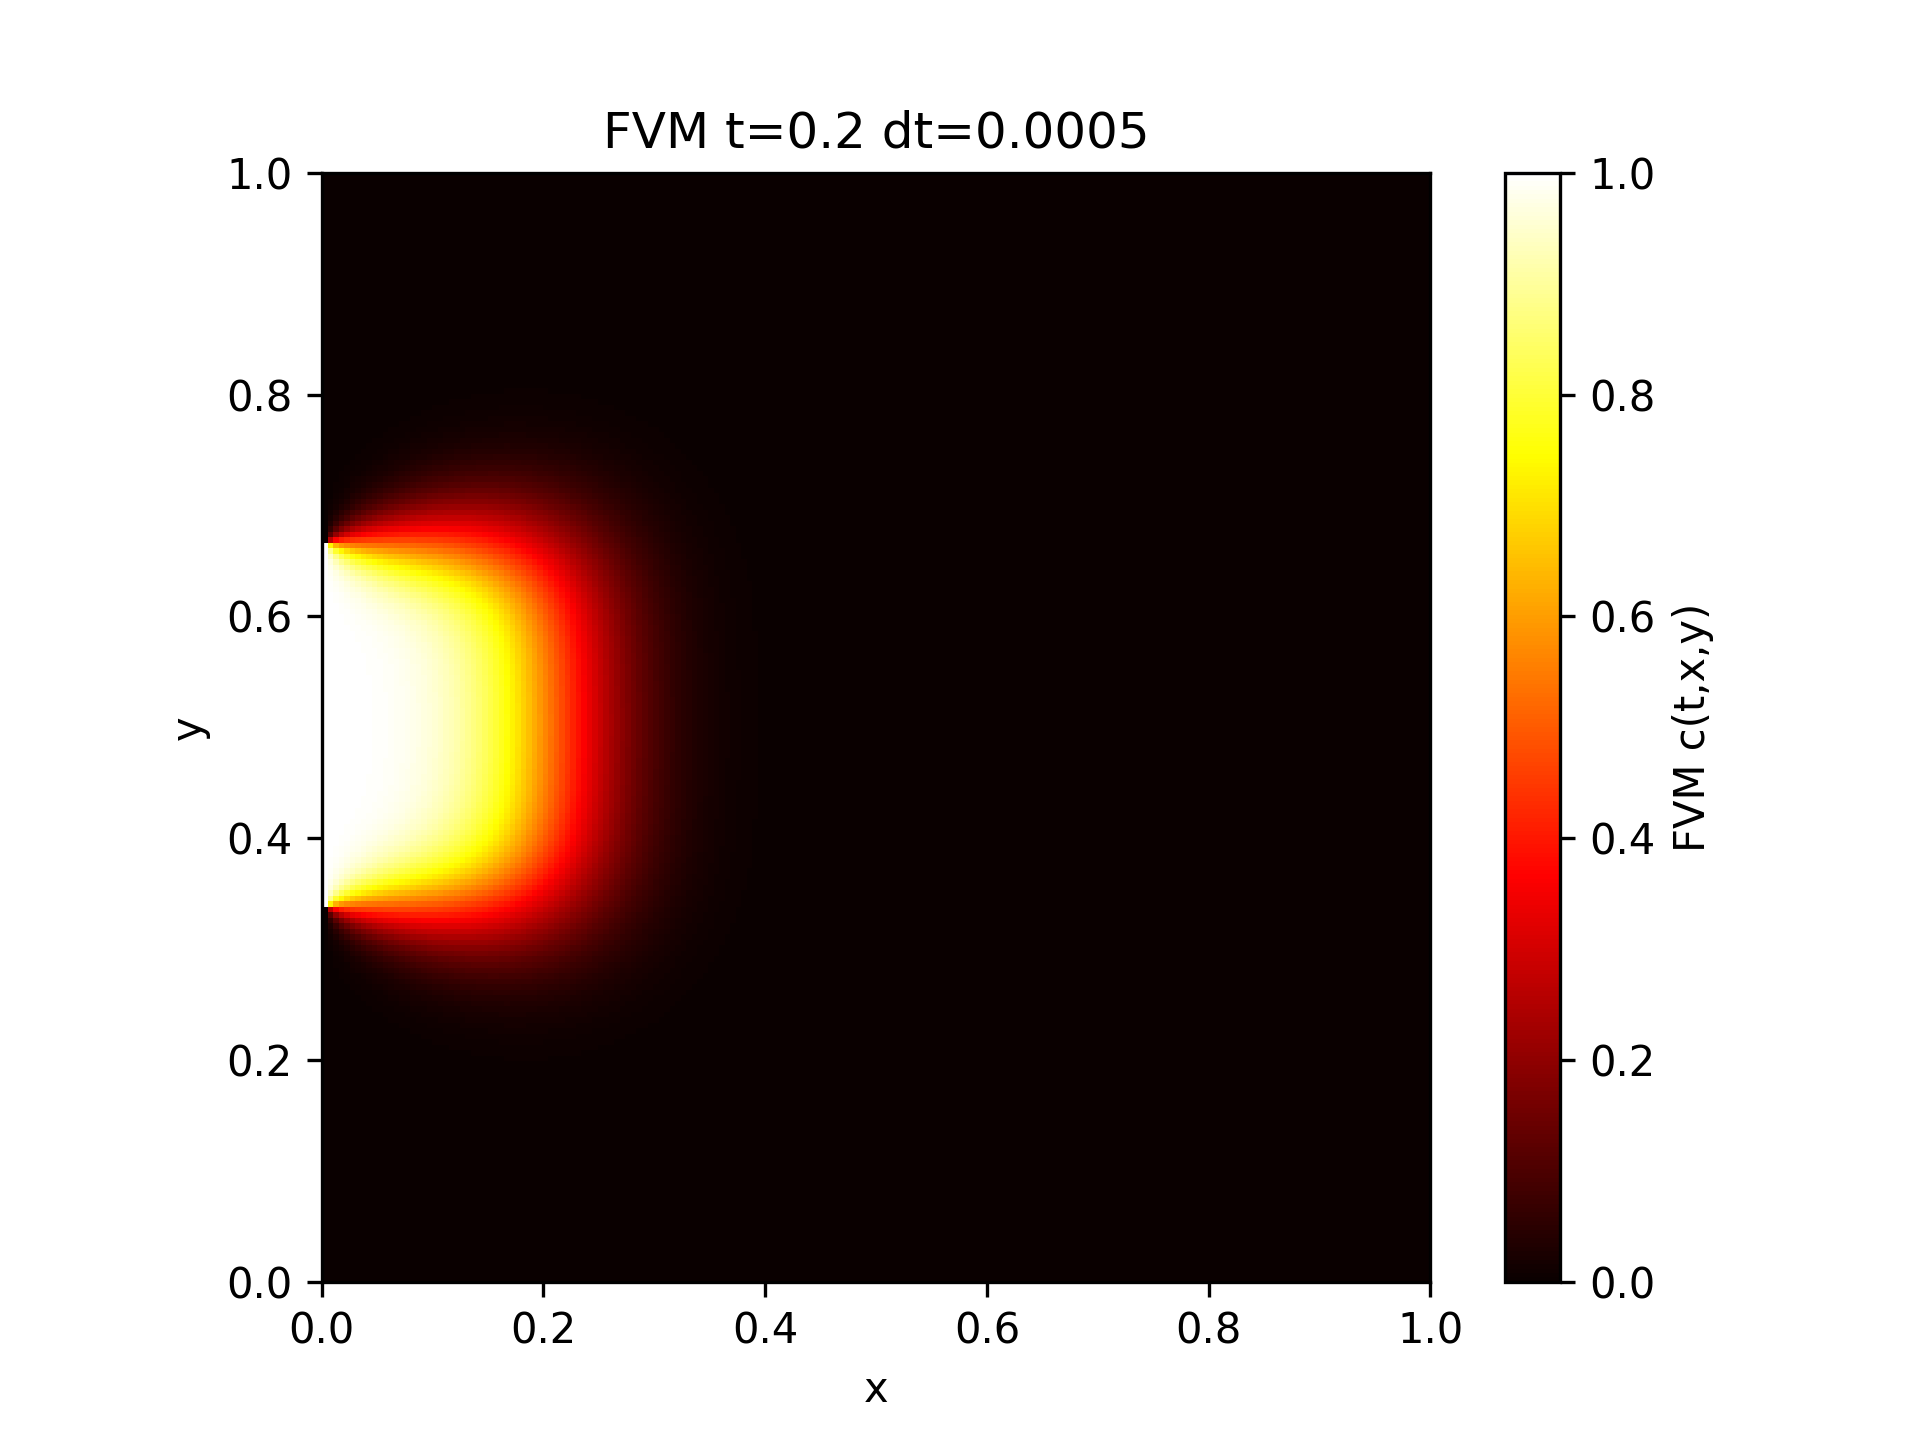
\includegraphics[width=\textwidth]{FVM t=0.2 dt=0.0005.png}
        \caption{FVM t=0.2 dt=0.0005}
        \label{FVM t=0.2 dt=0.0005}
    \end{subfigure}
    \hfill
    \begin{subfigure}{0.45\textwidth}
        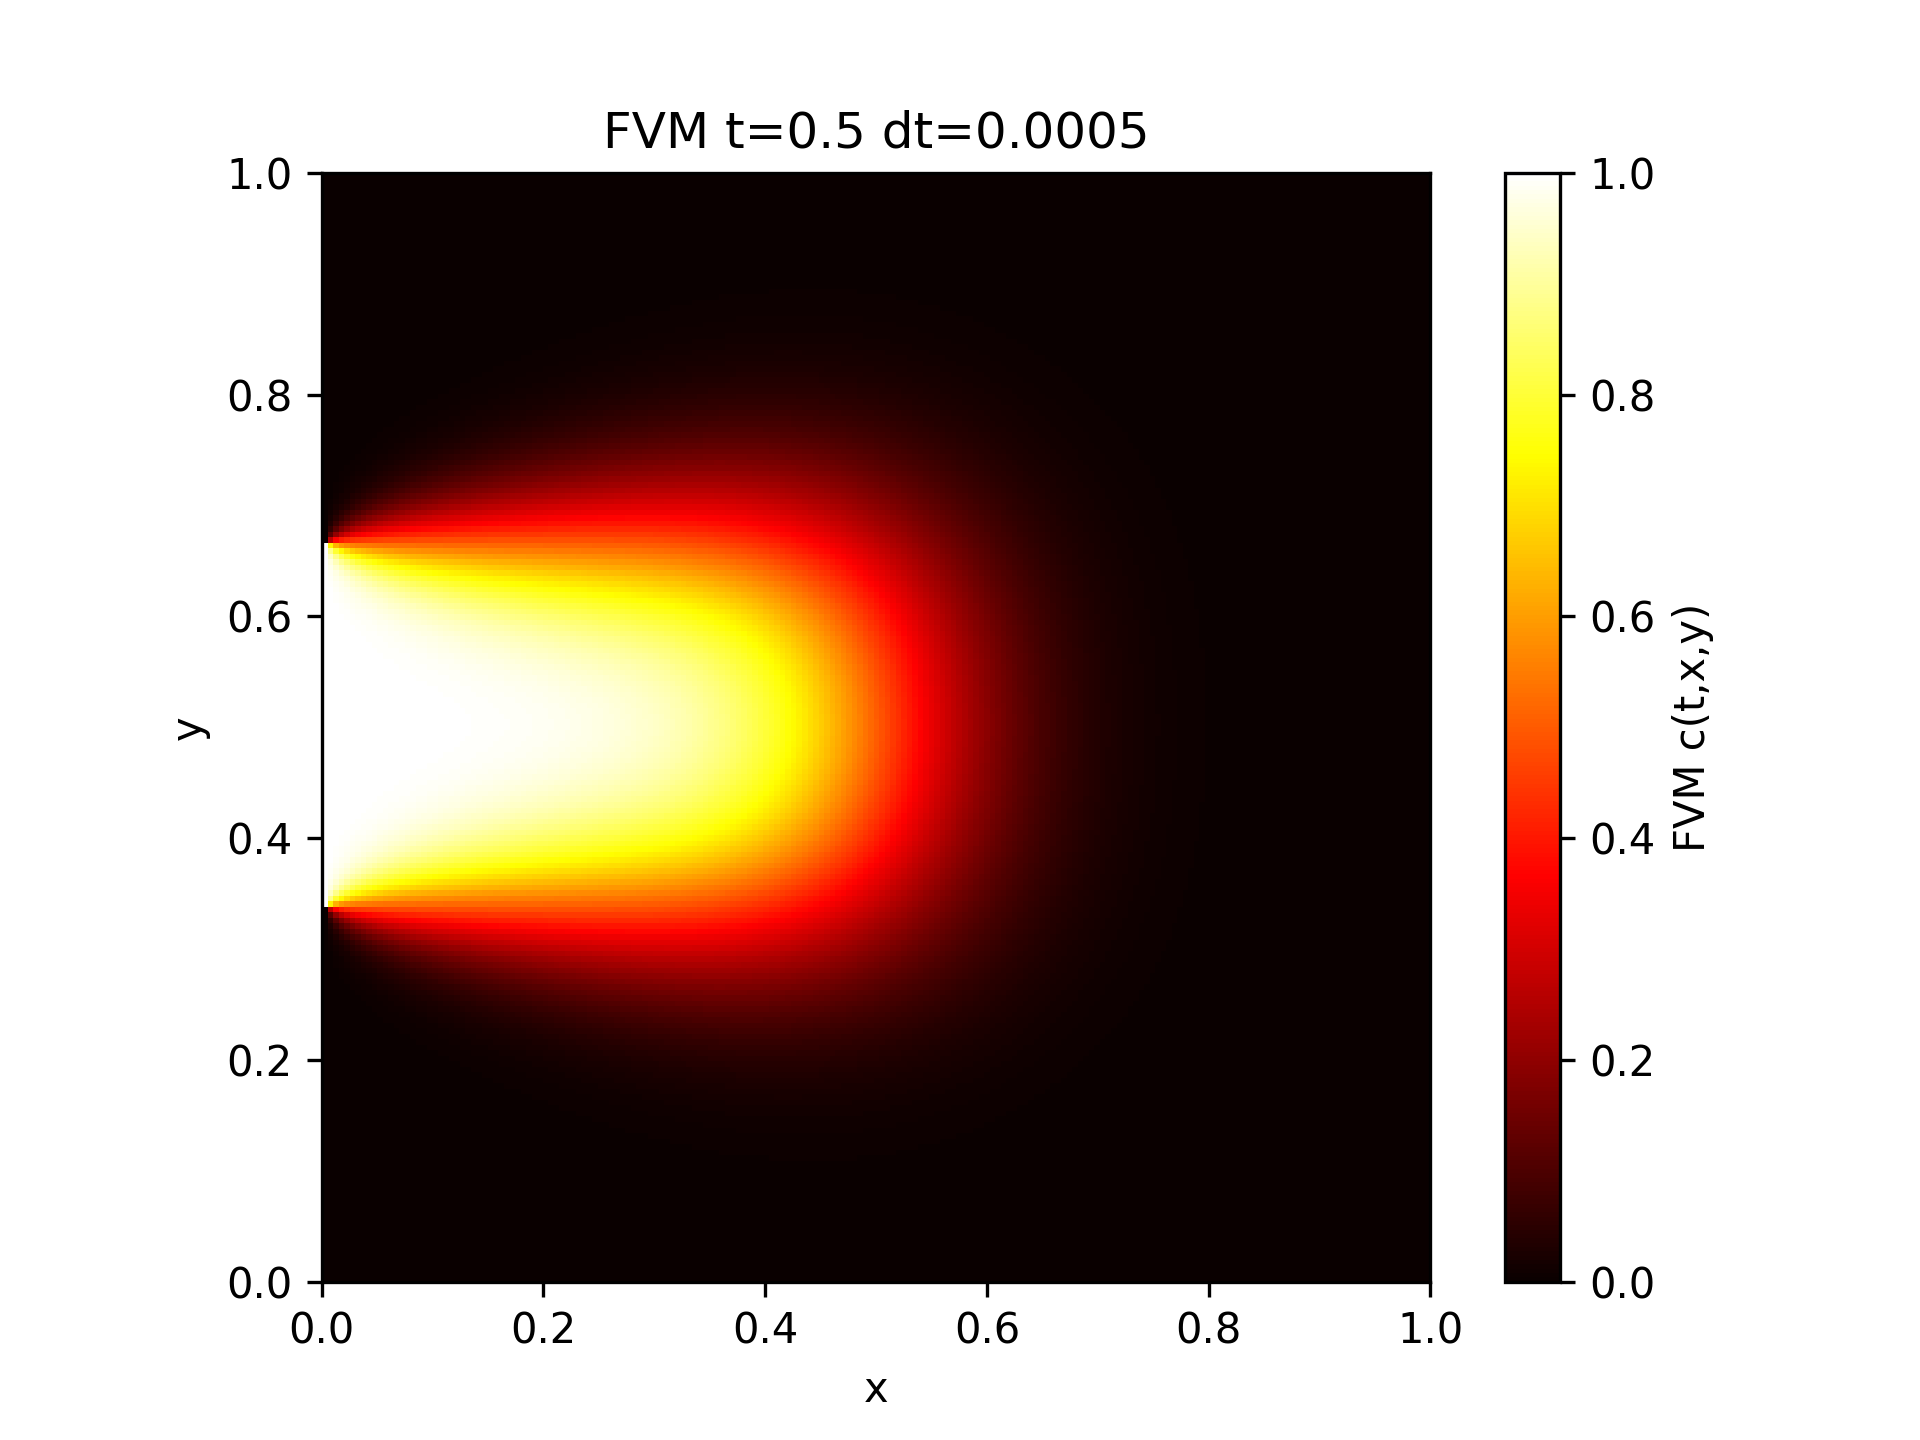
\includegraphics[width=\textwidth]{FVM t=0.5 dt=0.0005.png}
        \caption{FVM t=0.5 dt=0.0005}
        \label{FVM t=0.5 dt=0.0005}
    \end{subfigure}
    
    \vspace{0.5cm}  % 垂直间距
    
    \begin{subfigure}{0.45\textwidth}
        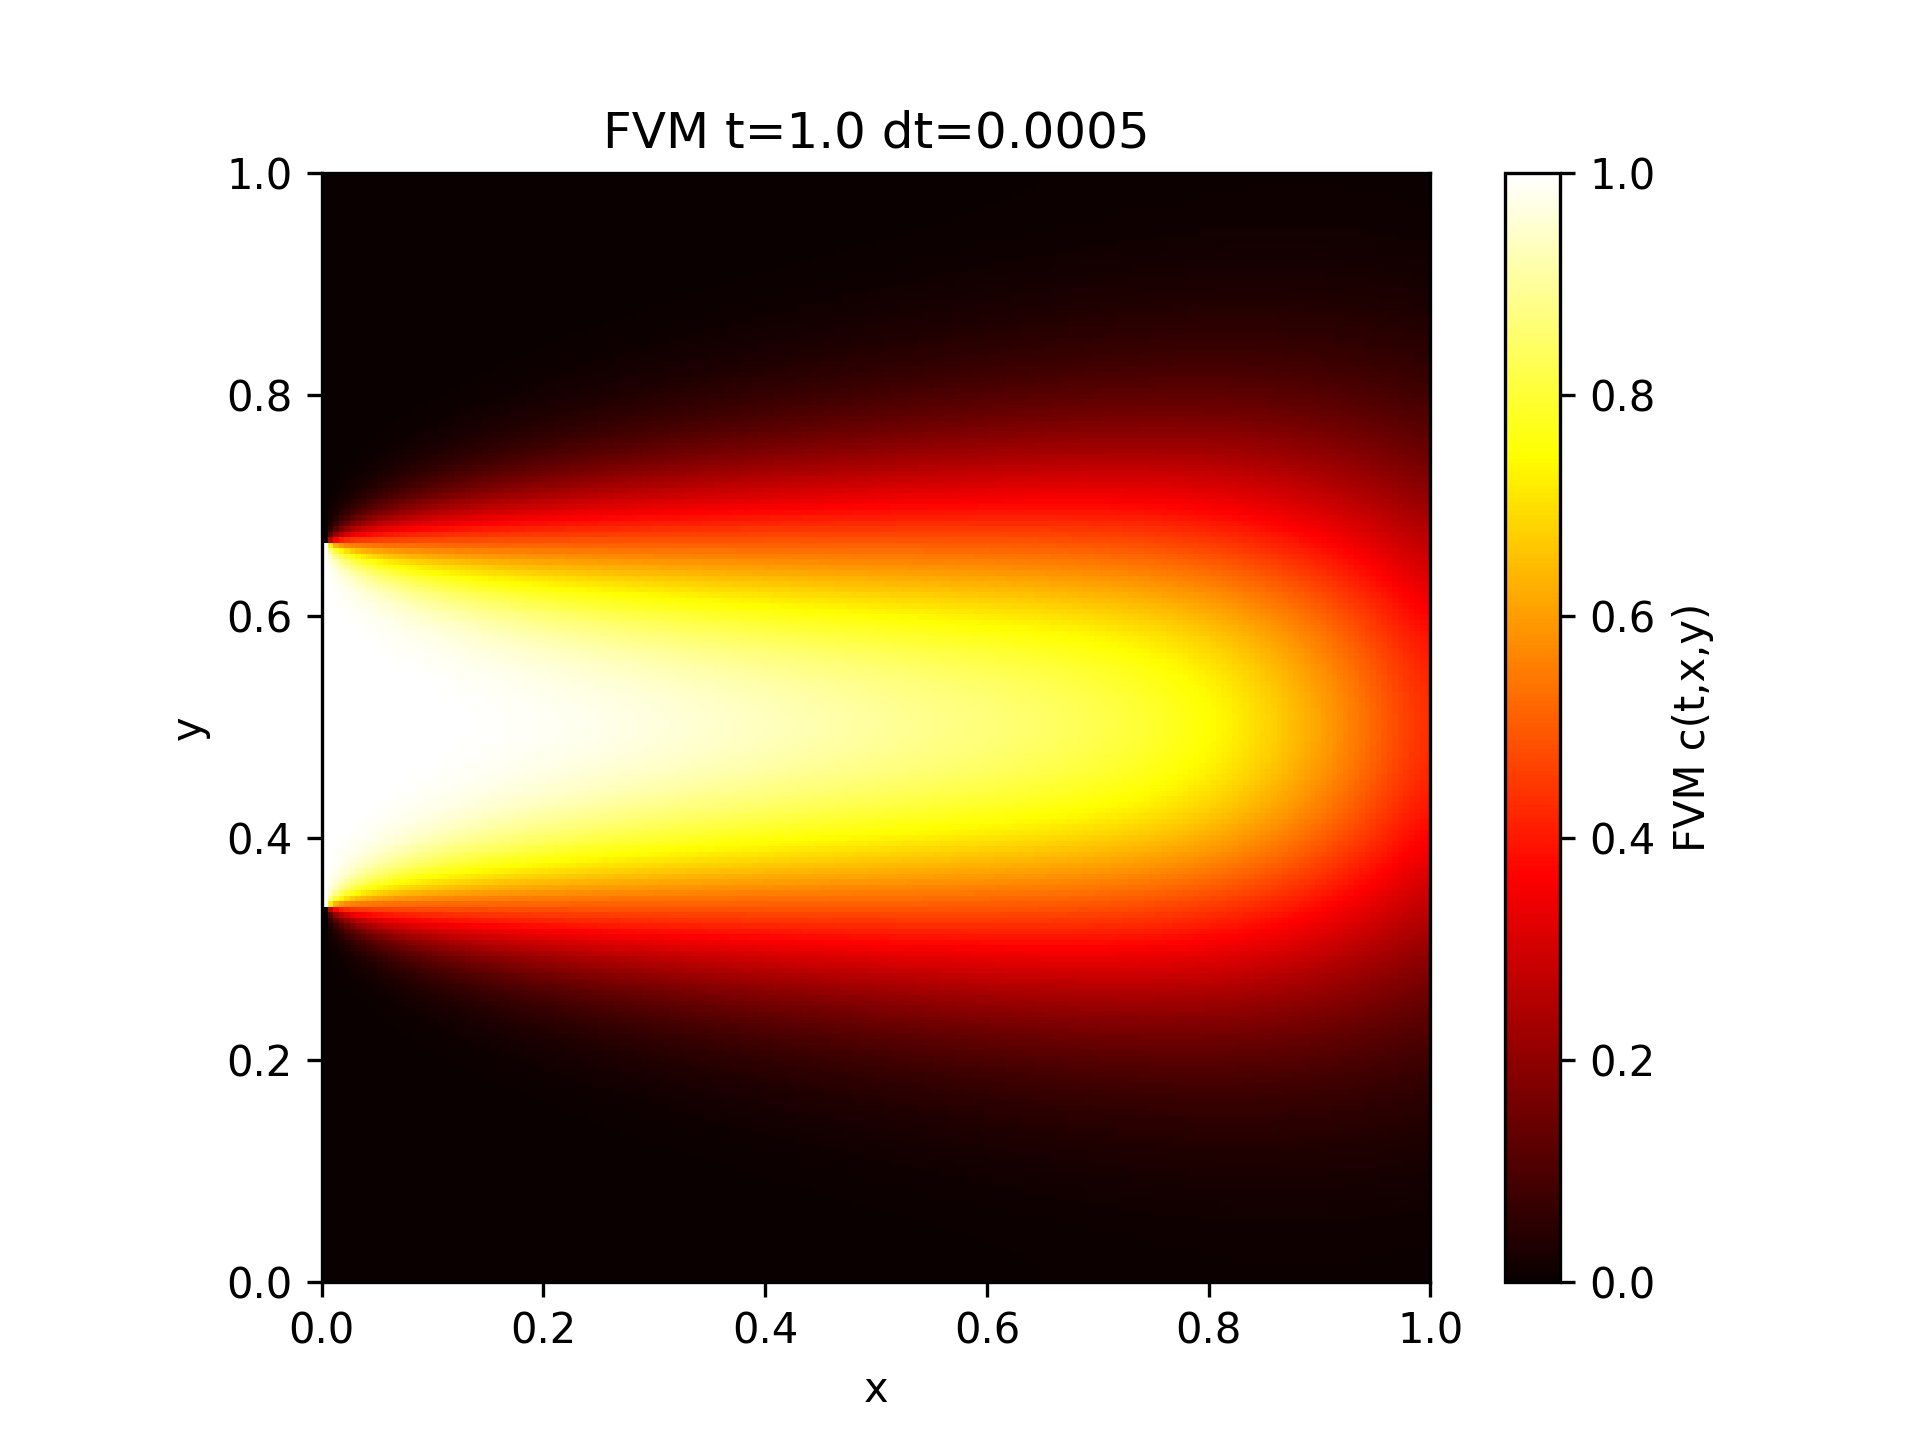
\includegraphics[width=\textwidth]{FVM t=1.0 dt=0.0005.png}
        \caption{FVM t=1.0 dt=0.0005}
        \label{FVM t=1.0 dt=0.0005}
    \end{subfigure}
    \hfill
    \begin{subfigure}{0.45\textwidth}
        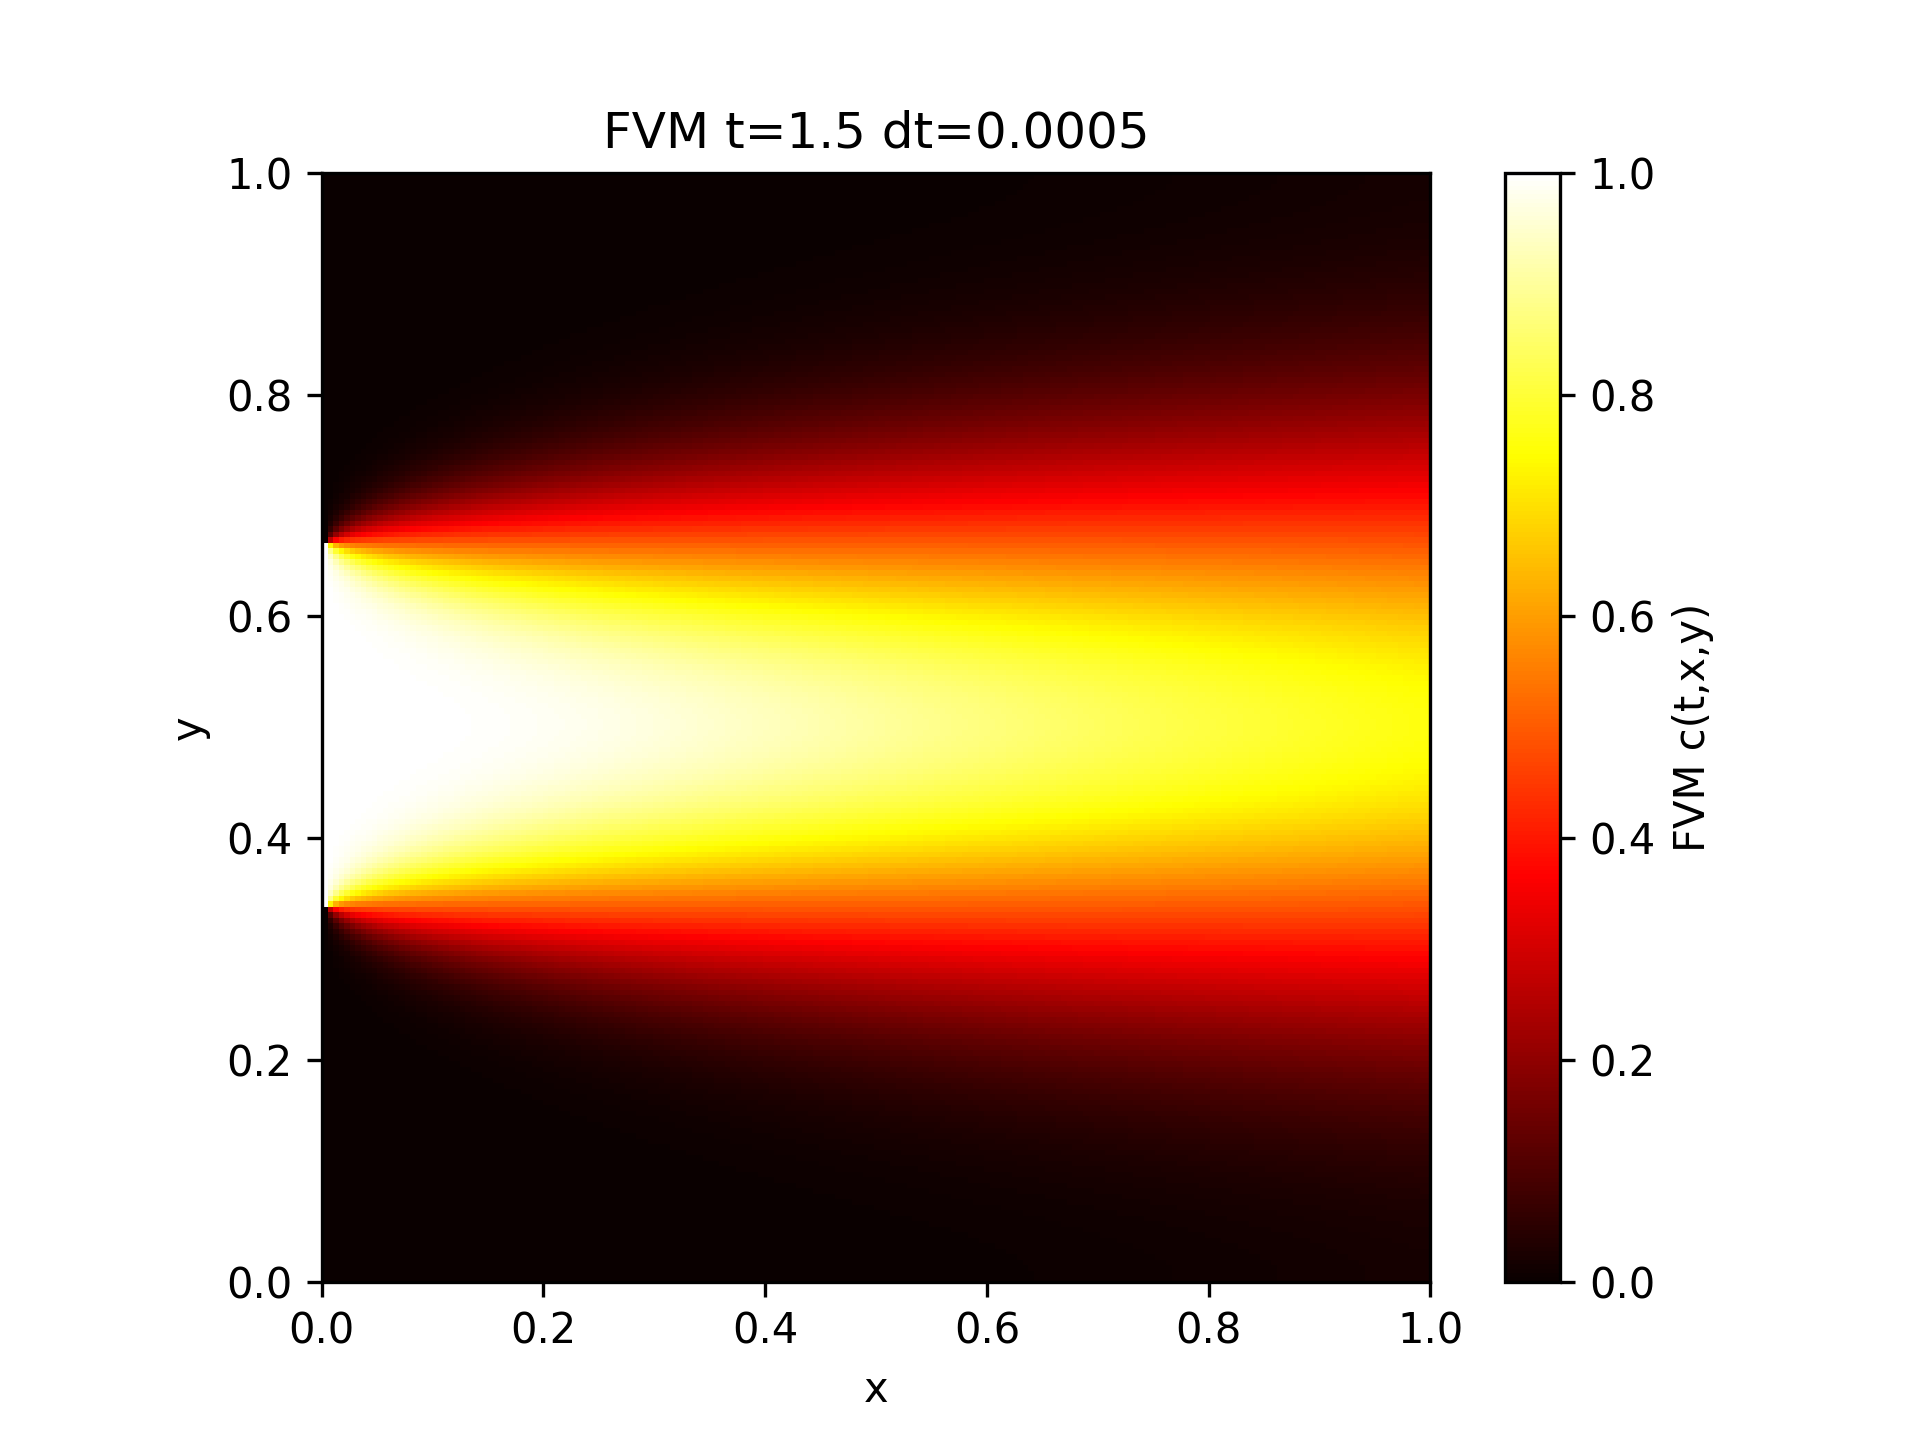
\includegraphics[width=\textwidth]{FVM t=1.5 dt=0.0005.png}
        \caption{FVM t=1.5 dt=0.0005}
        \label{FVM t=1.5 dt=0.0005}
    \end{subfigure}
    
    \caption{results of FVM dt = 0.0005}
    \label{results of FVM dt = 0.0005}
\end{figure}

\begin{figure}[htbp]
    \centering
    % 2x2 排列
    \begin{subfigure}{0.45\textwidth}
        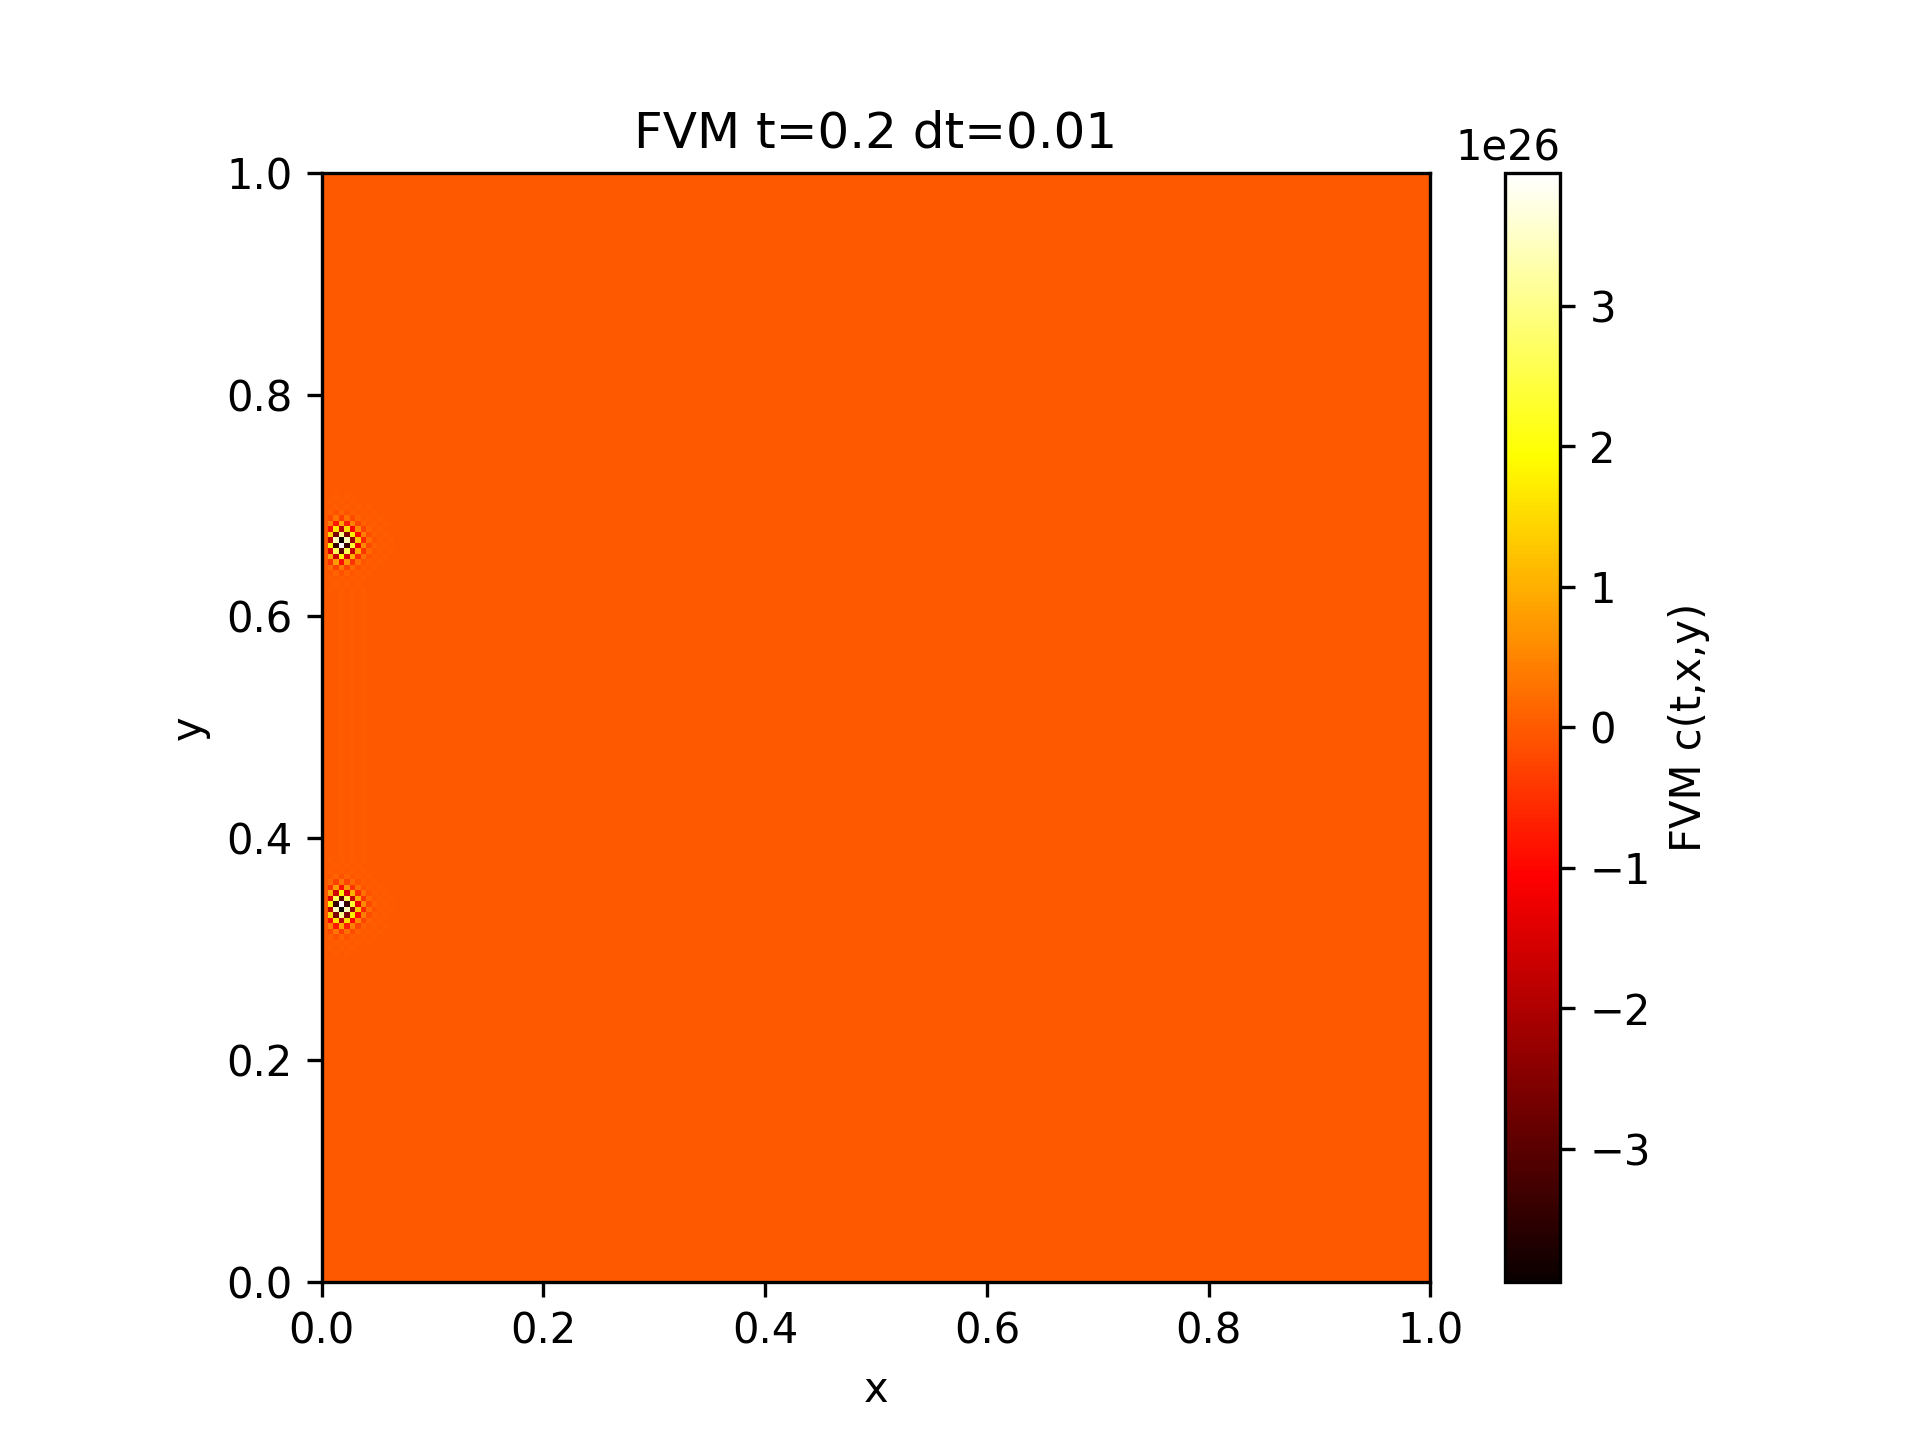
\includegraphics[width=\textwidth]{FVM t=0.2 dt=0.01.png}
        \caption{FVM t=0.2 dt=0.01}
        \label{FVM t=0.2 dt=0.01}
    \end{subfigure}
    \hfill
    \begin{subfigure}{0.45\textwidth}
        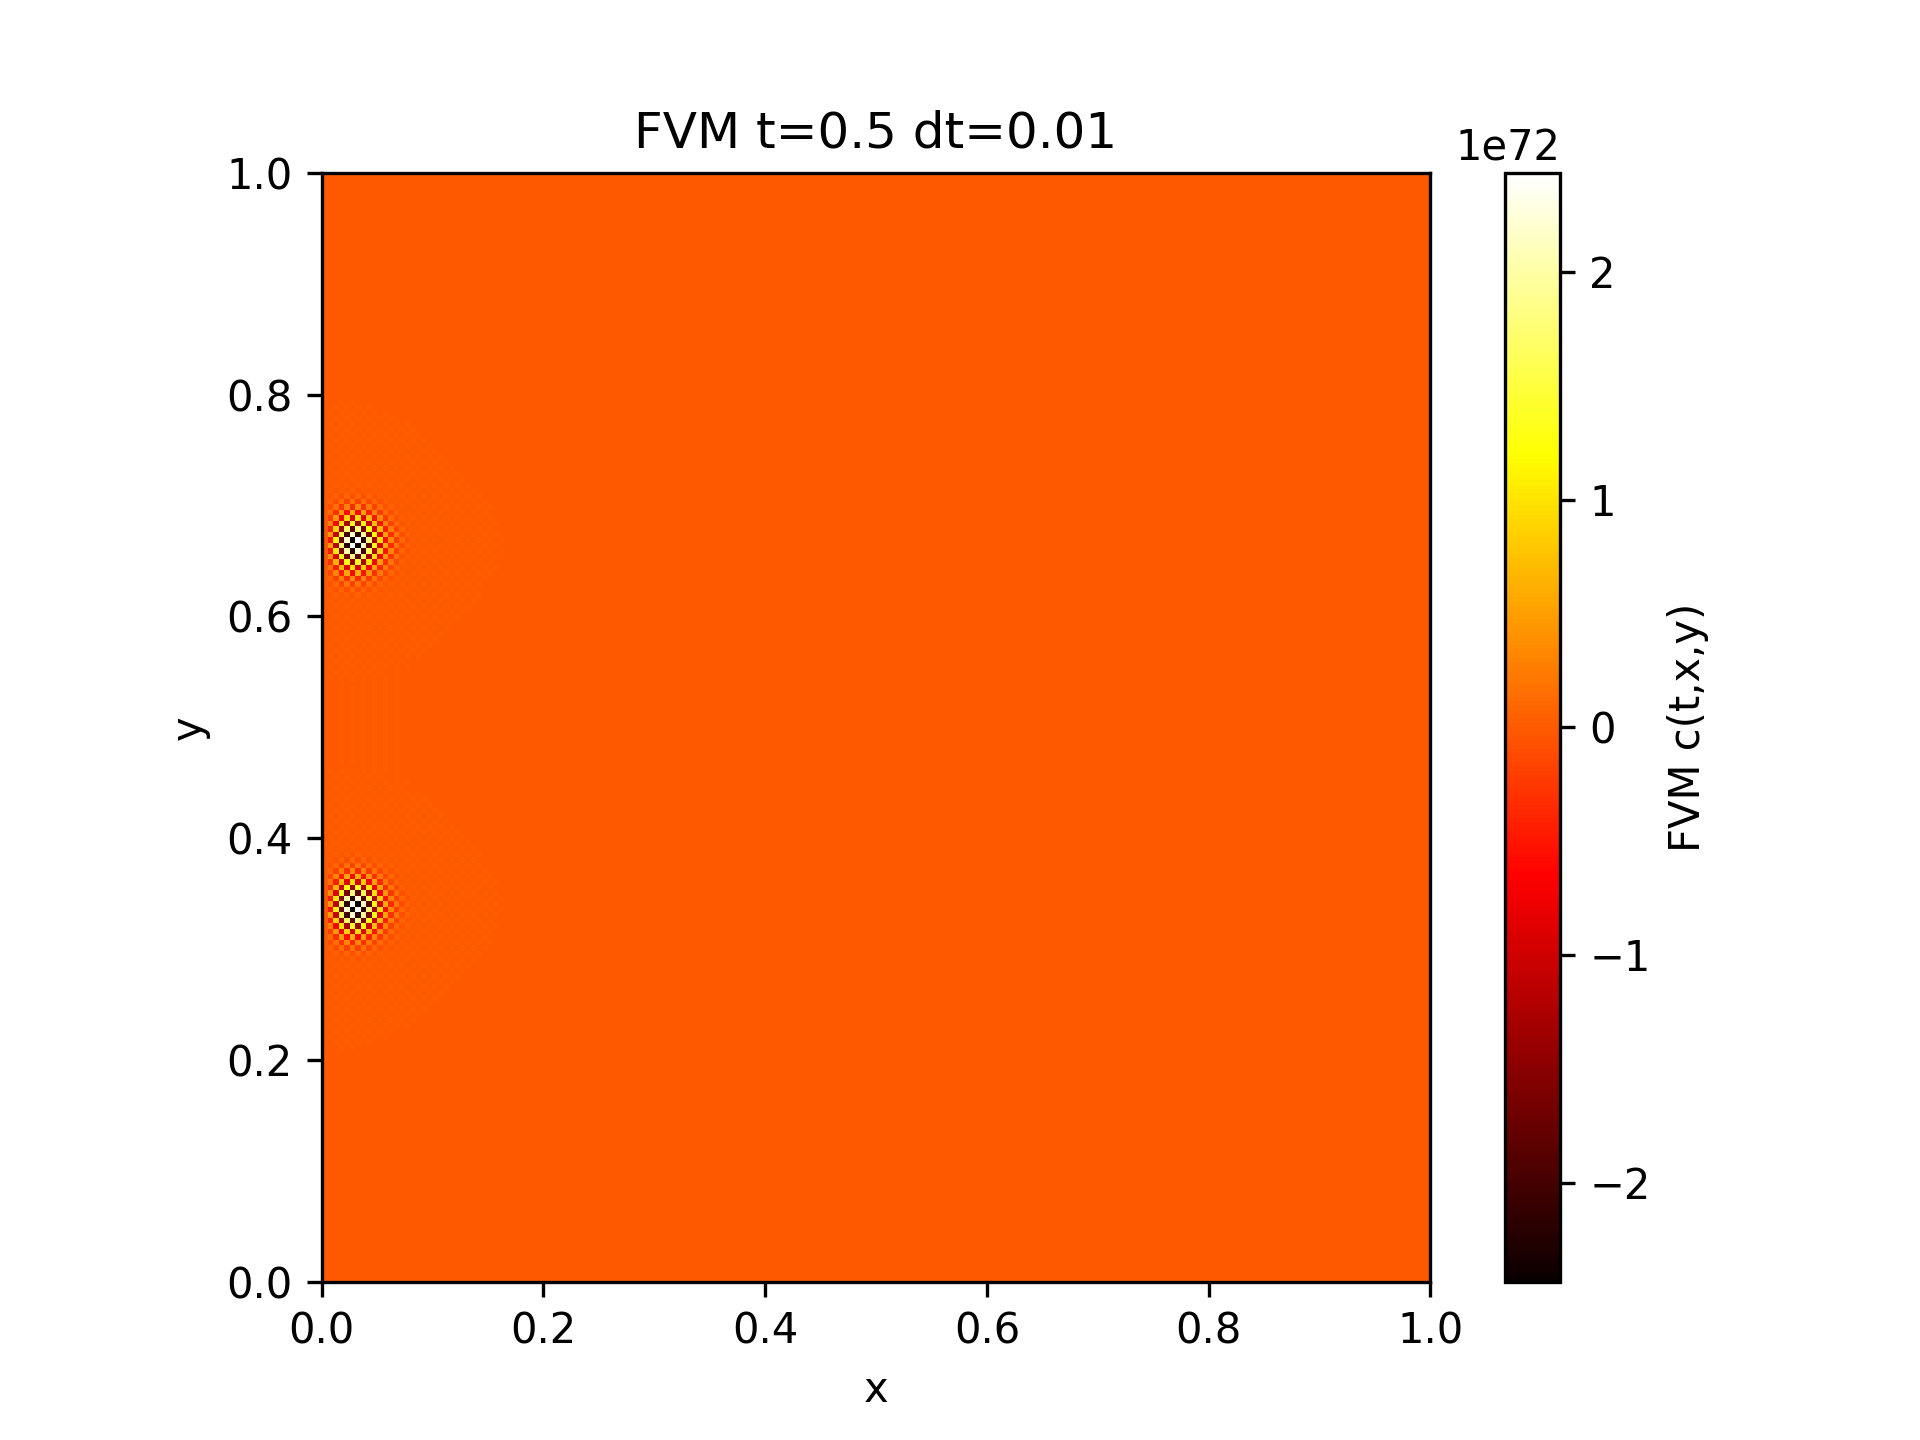
\includegraphics[width=\textwidth]{FVM t=0.5 dt=0.01.png}
        \caption{FVM t=0.5 dt=0.01}
        \label{FVM t=0.5 dt=0.01}
    \end{subfigure}
    
    \vspace{0.5cm}  % 垂直间距
    
    \begin{subfigure}{0.45\textwidth}
        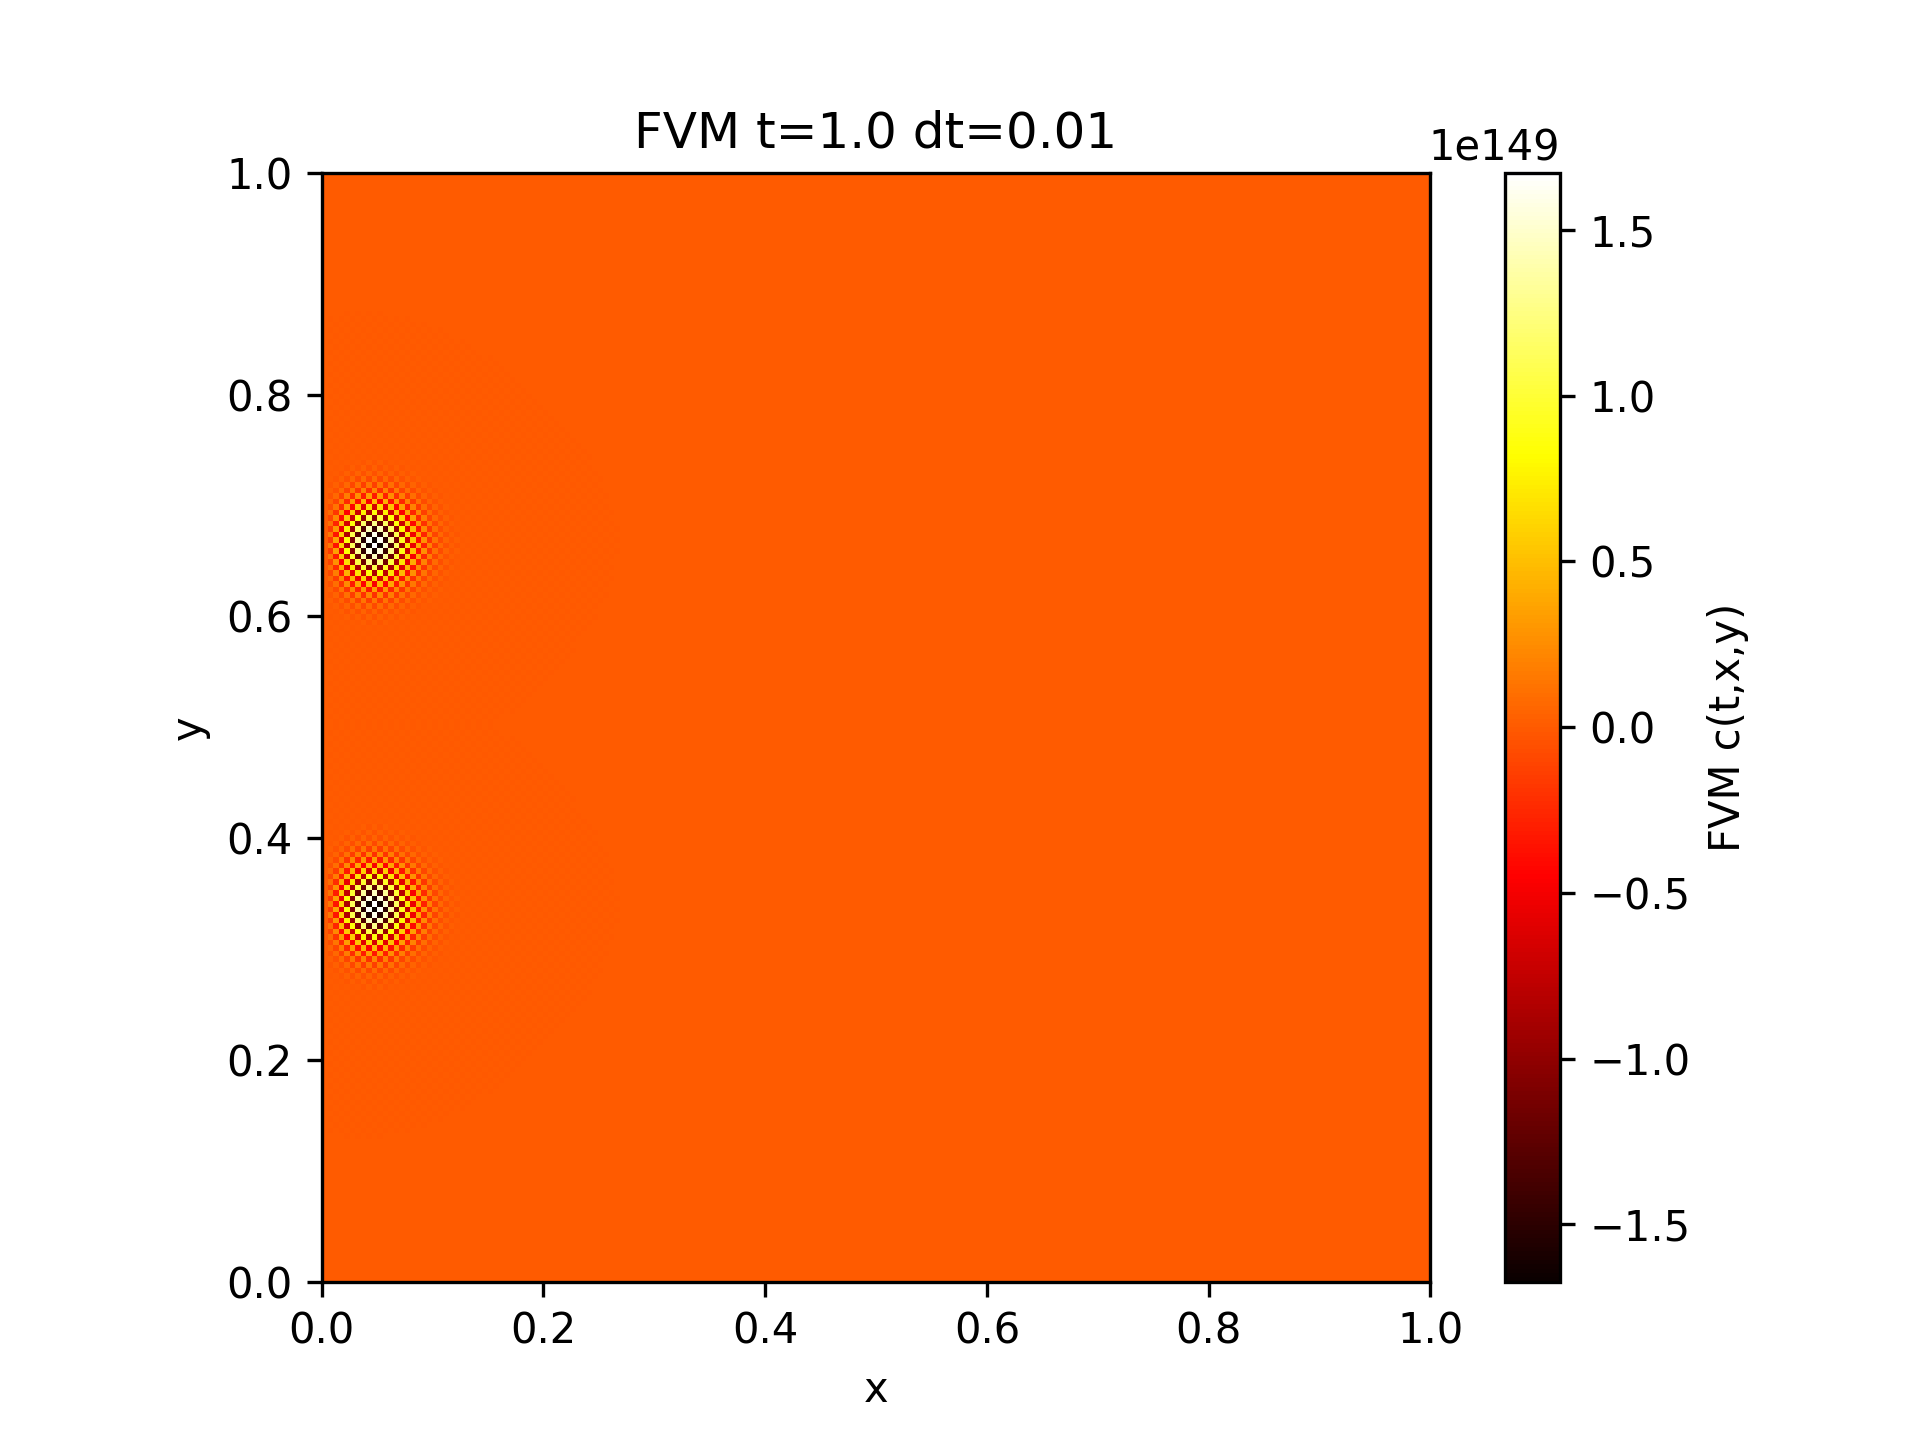
\includegraphics[width=\textwidth]{FVM t=1.0 dt=0.01.png}
        \caption{FVM t=1.0 dt=0.01}
        \label{FVM t=1.0 dt=0.01}
    \end{subfigure}
    \hfill
    \begin{subfigure}{0.45\textwidth}
        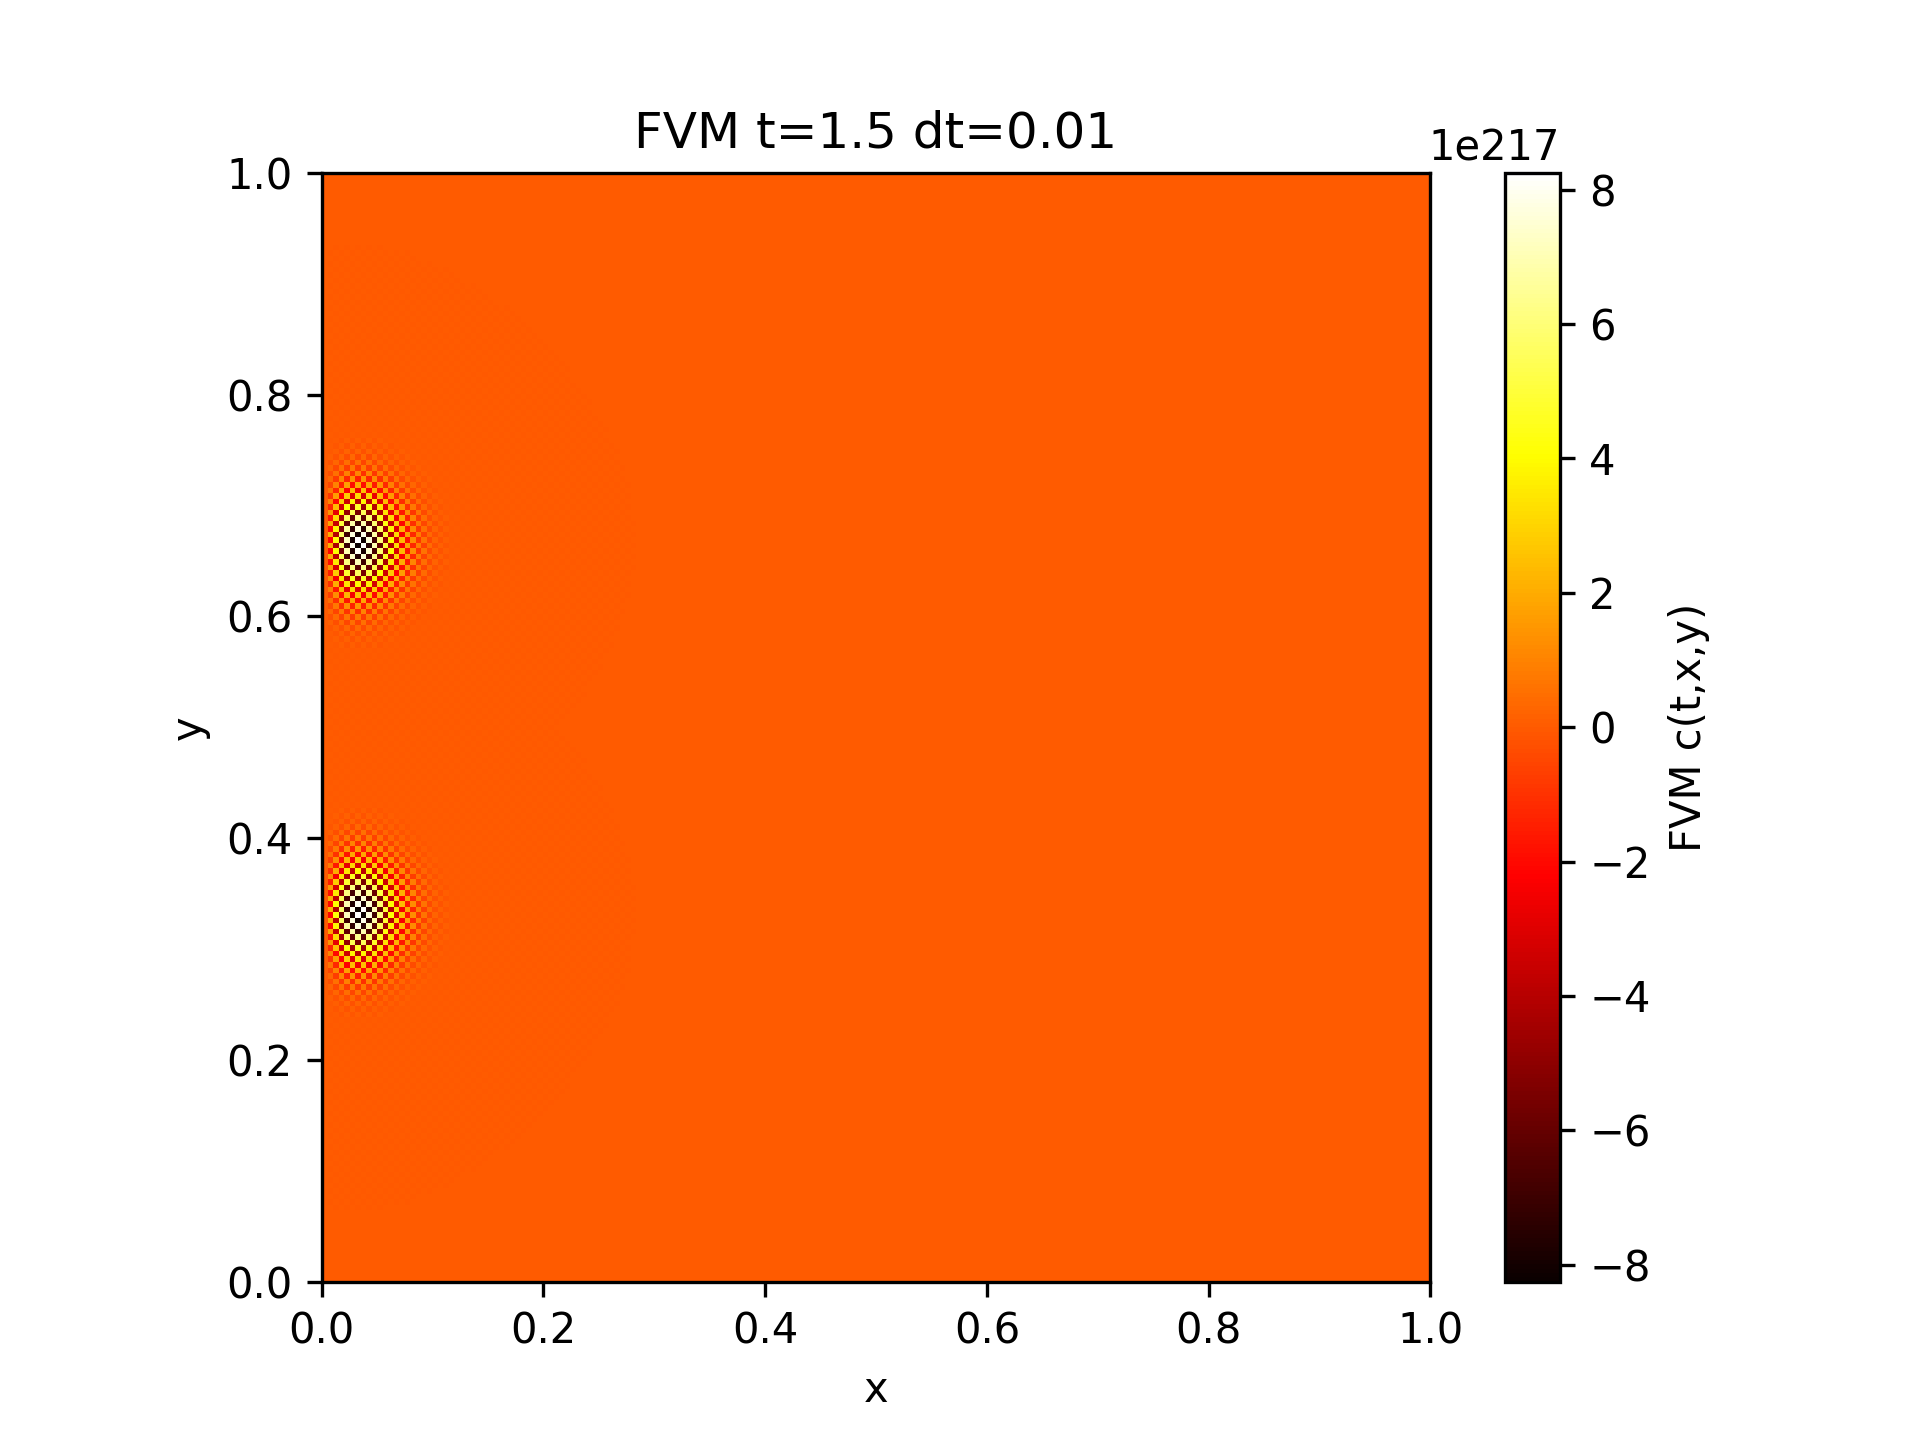
\includegraphics[width=\textwidth]{FVM t=1.5 dt=0.01.png}
        \caption{FVM t=1.5 dt=0.01}
        \label{FVM t=1.5 dt=0.01}
    \end{subfigure}
    \caption{results of FVM dt = 0.01}
    \label{results of FVM dt = 0.01}
\end{figure}
\section{问题2}
采用基于正交分解的降阶模型对上述问题进行计算.首先写出离散后的方程\begin{equation}
    \frac{\partial \mathbf{c}}{\partial t} = A\mathbf{c}+f
\end{equation}
其中$A$是对流扩散方程离散后的矩阵,$f$是边界条件的作用。
\subsection{计算格式}
取定$N_{snap} = 100$,对$[0,T]$做等距划分,得到数据集,对其用梯形公式做积分近似,进而得到快照矩阵$S$.设定基底维数为$k$,对$S$做SVD分解,取左奇异向量矩阵的前$k$列
为投影基底矩阵$V$.做低秩近似$\mathbf{c} = V\mathbf{q}$,进而有\begin{equation}
    \begin{cases}
        \frac{\partial \mathbf{q}}{\partial t} = V^{T}AV\mathbf{q}+V^{T}f
        \\
        \mathbf{c} = V\mathbf{q}
    \end{cases}
\end{equation}
用一阶向前Euler求解关于$\mathbf{q}$的ODE,进而计算$\mathbf{c}$。
\par 子函数求解矩阵-向量乘法$Ax$,与FVM中格式基本类似,只是需要单独处理$i=0$的情况:左端来自左边界,即$f$的作用.
\subsection{时间步长}
采用时间步长$dt = 5e-4$,与FVM中一致。
\subsection{不同基底数量下的结果展示}
设置基底数量$k=2,5,10,15$,计算结果分别展示如图\ref{results of POD k = 2}、\ref{results of POD k = 5}、
\ref{results of POD k = 10}、\ref{results of POD k = 15}所示。
\begin{figure}[htbp]
    \centering
    % 2x2 排列
    \begin{subfigure}{0.45\textwidth}
        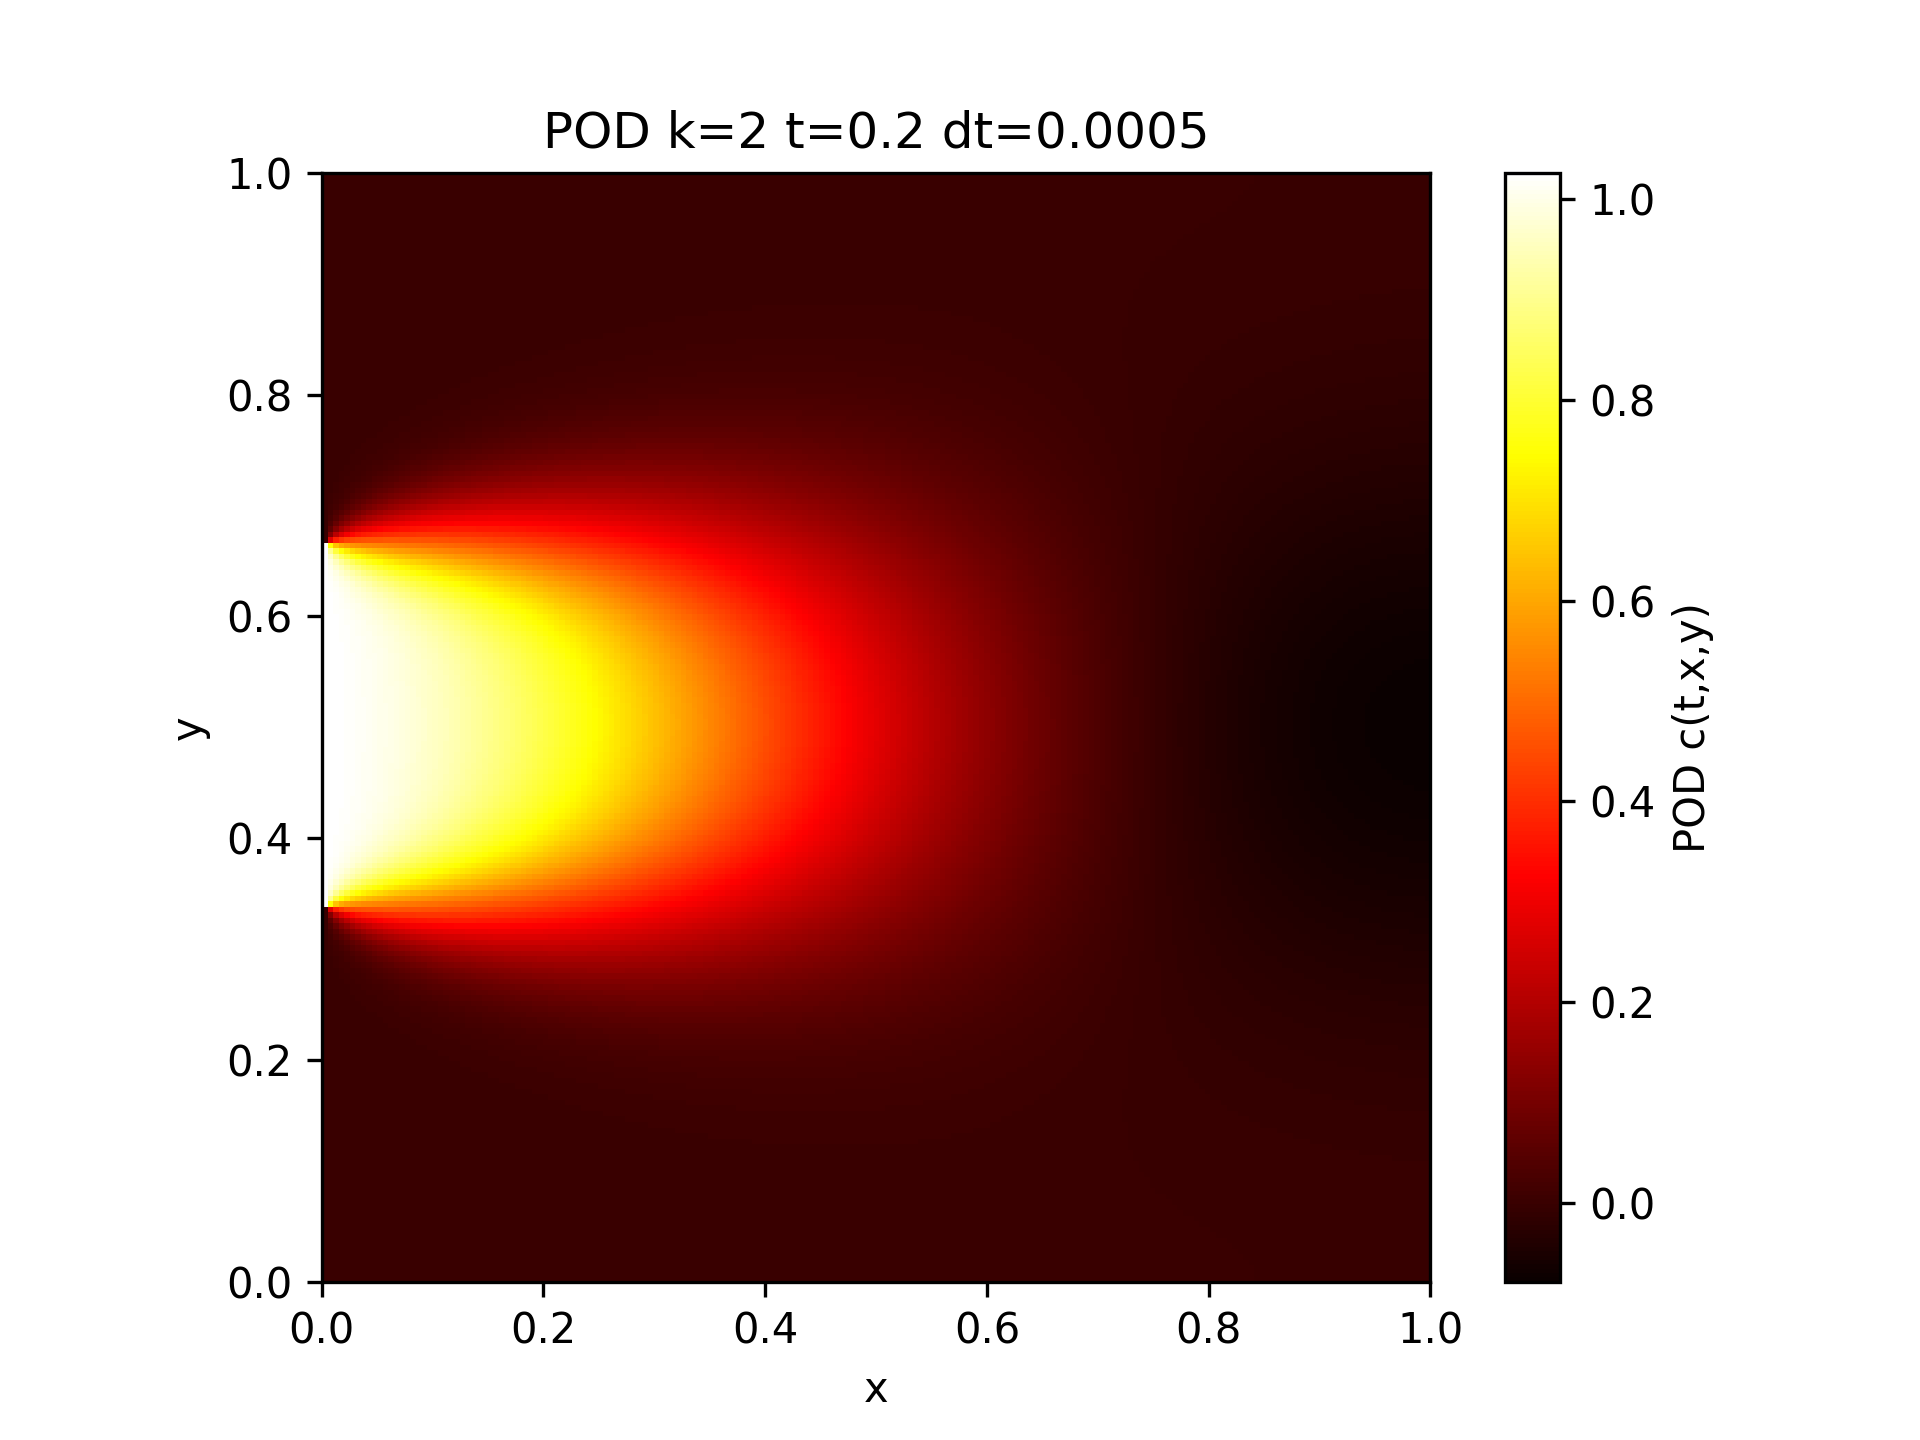
\includegraphics[width=\textwidth]{POD k=2 t=0.2 dt=0.0005.png}
        \caption{POD k=2 t=0.2 dt=0.0005}
        \label{POD k=2 t=0.2 dt=0.0005}
    \end{subfigure}
    \hfill
    \begin{subfigure}{0.45\textwidth}
        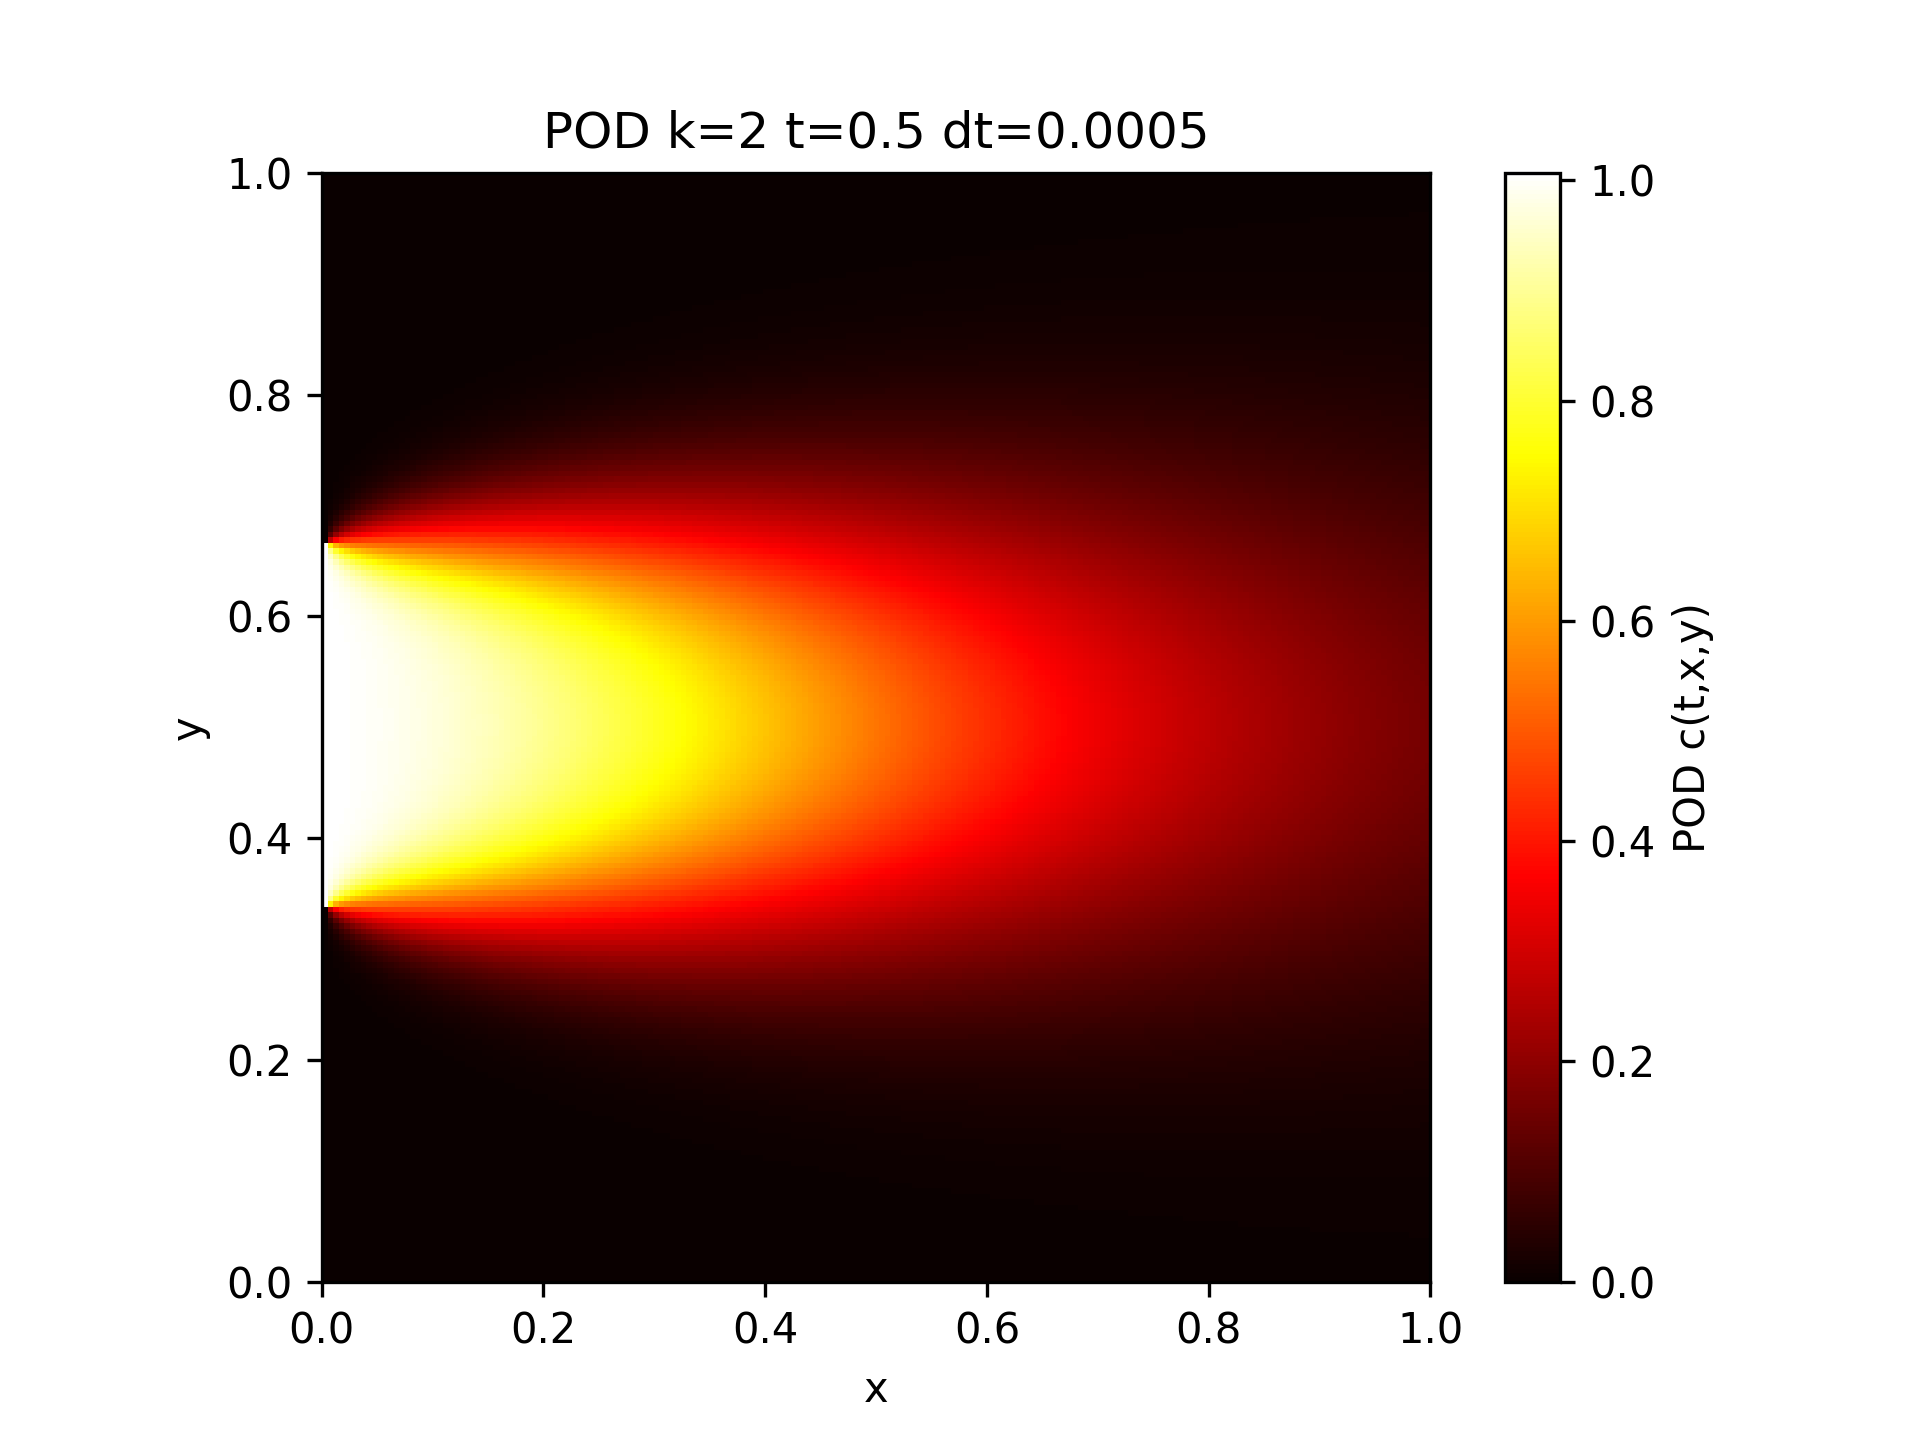
\includegraphics[width=\textwidth]{POD k=2 t=0.5 dt=0.0005.png}
        \caption{POD k=2 t=0.5 dt=0.0005}
        \label{POD k=2 t=0.5 dt=0.0005}
    \end{subfigure}
    
    \vspace{0.5cm}  % 垂直间距
    
    \begin{subfigure}{0.45\textwidth}
        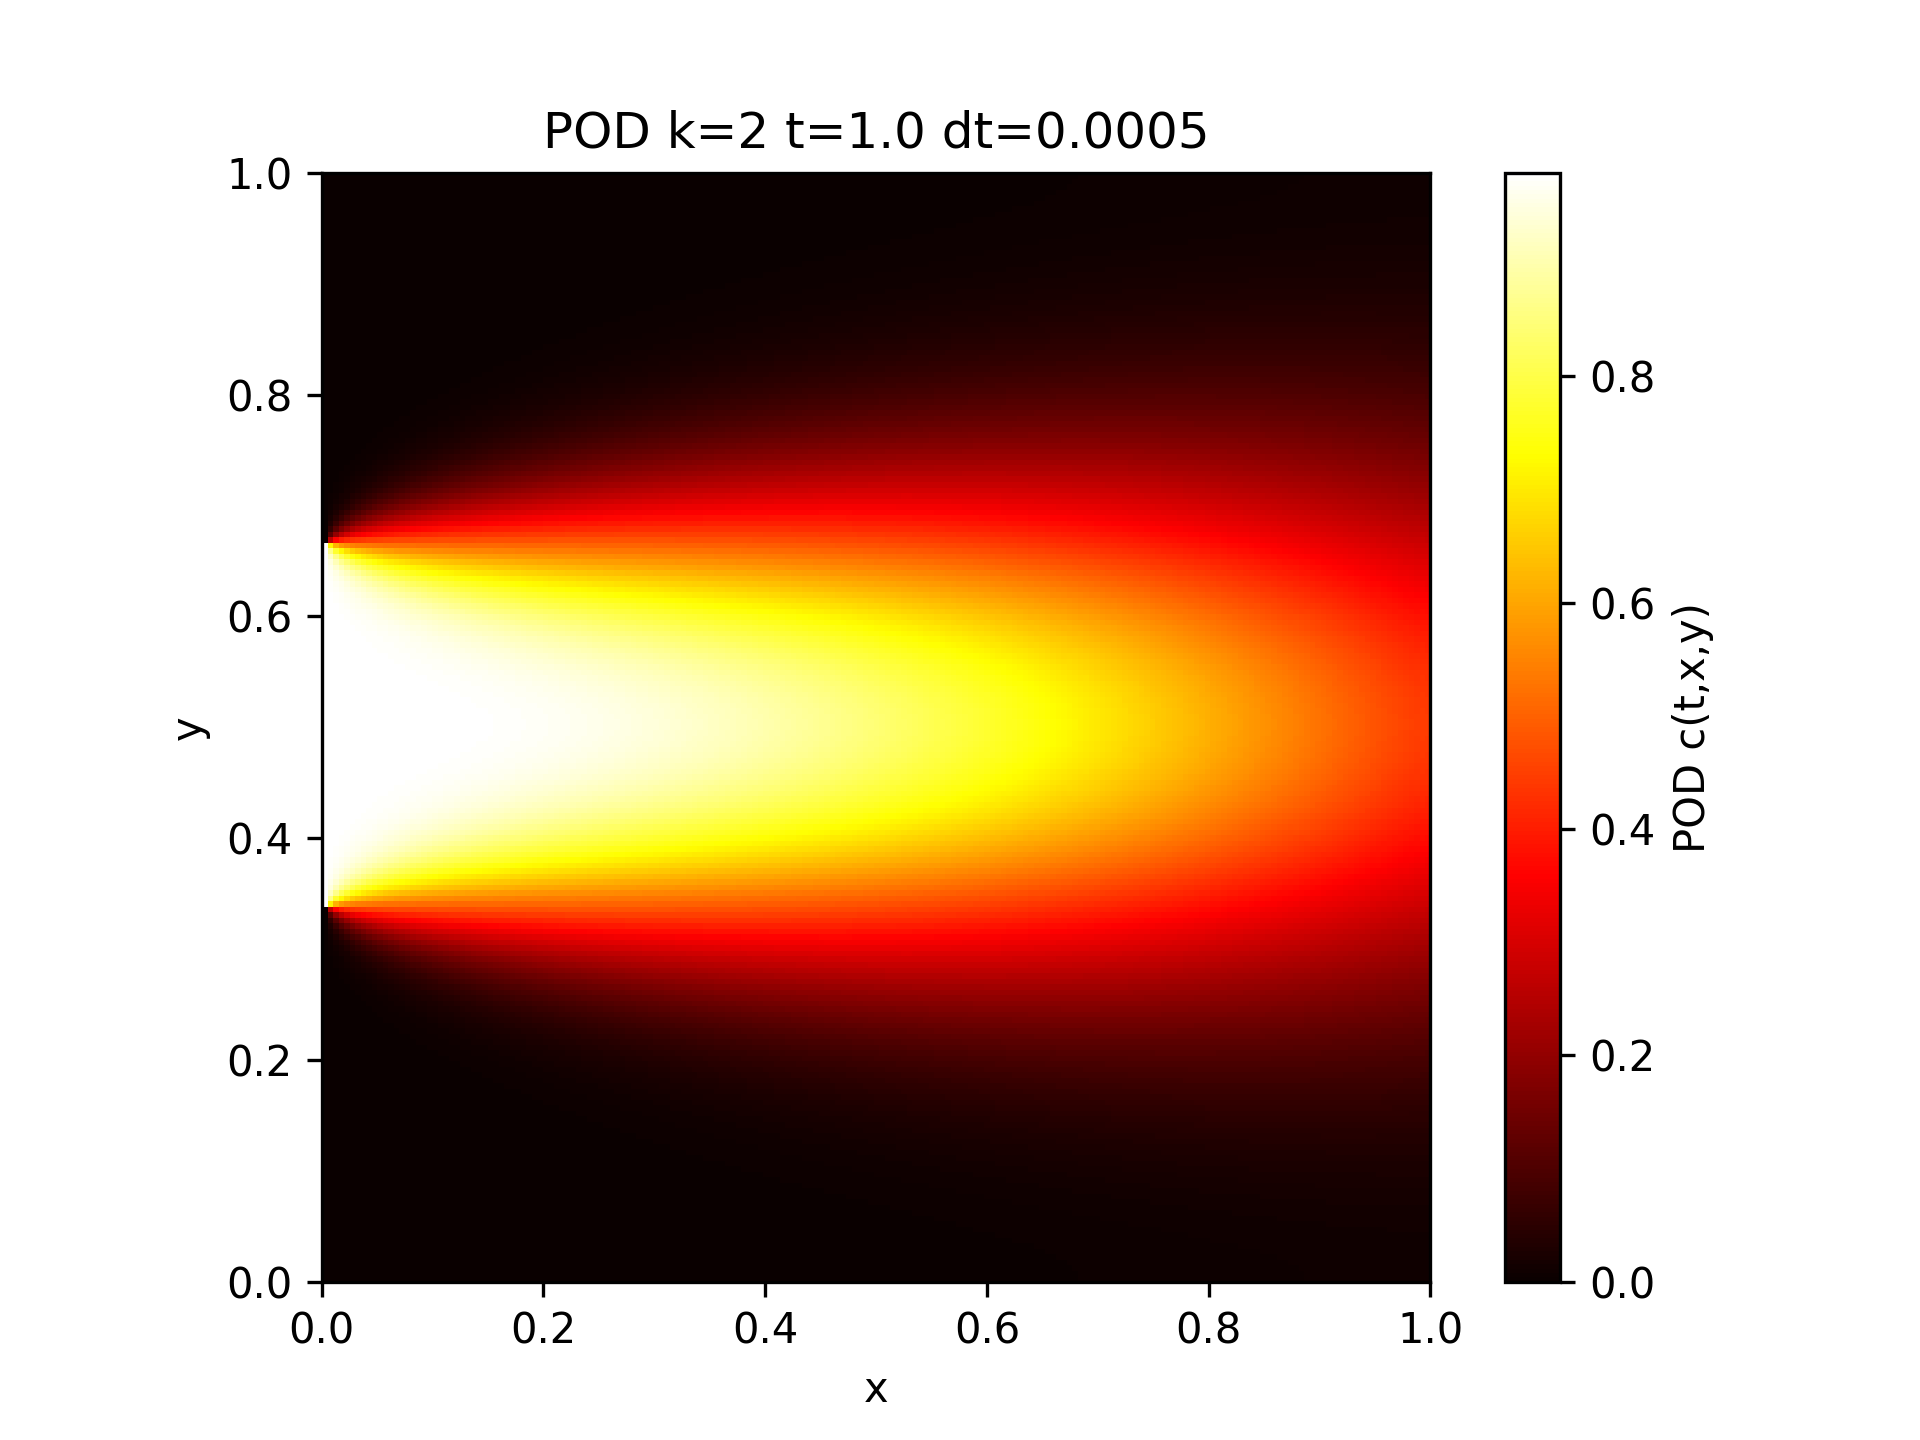
\includegraphics[width=\textwidth]{POD k=2 t=1.0 dt=0.0005.png}
        \caption{POD k=2 t=1.0 dt=0.0005}
        \label{POD k=2 t=1.0 dt=0.0005}
    \end{subfigure}
    \hfill
    \begin{subfigure}{0.45\textwidth}
        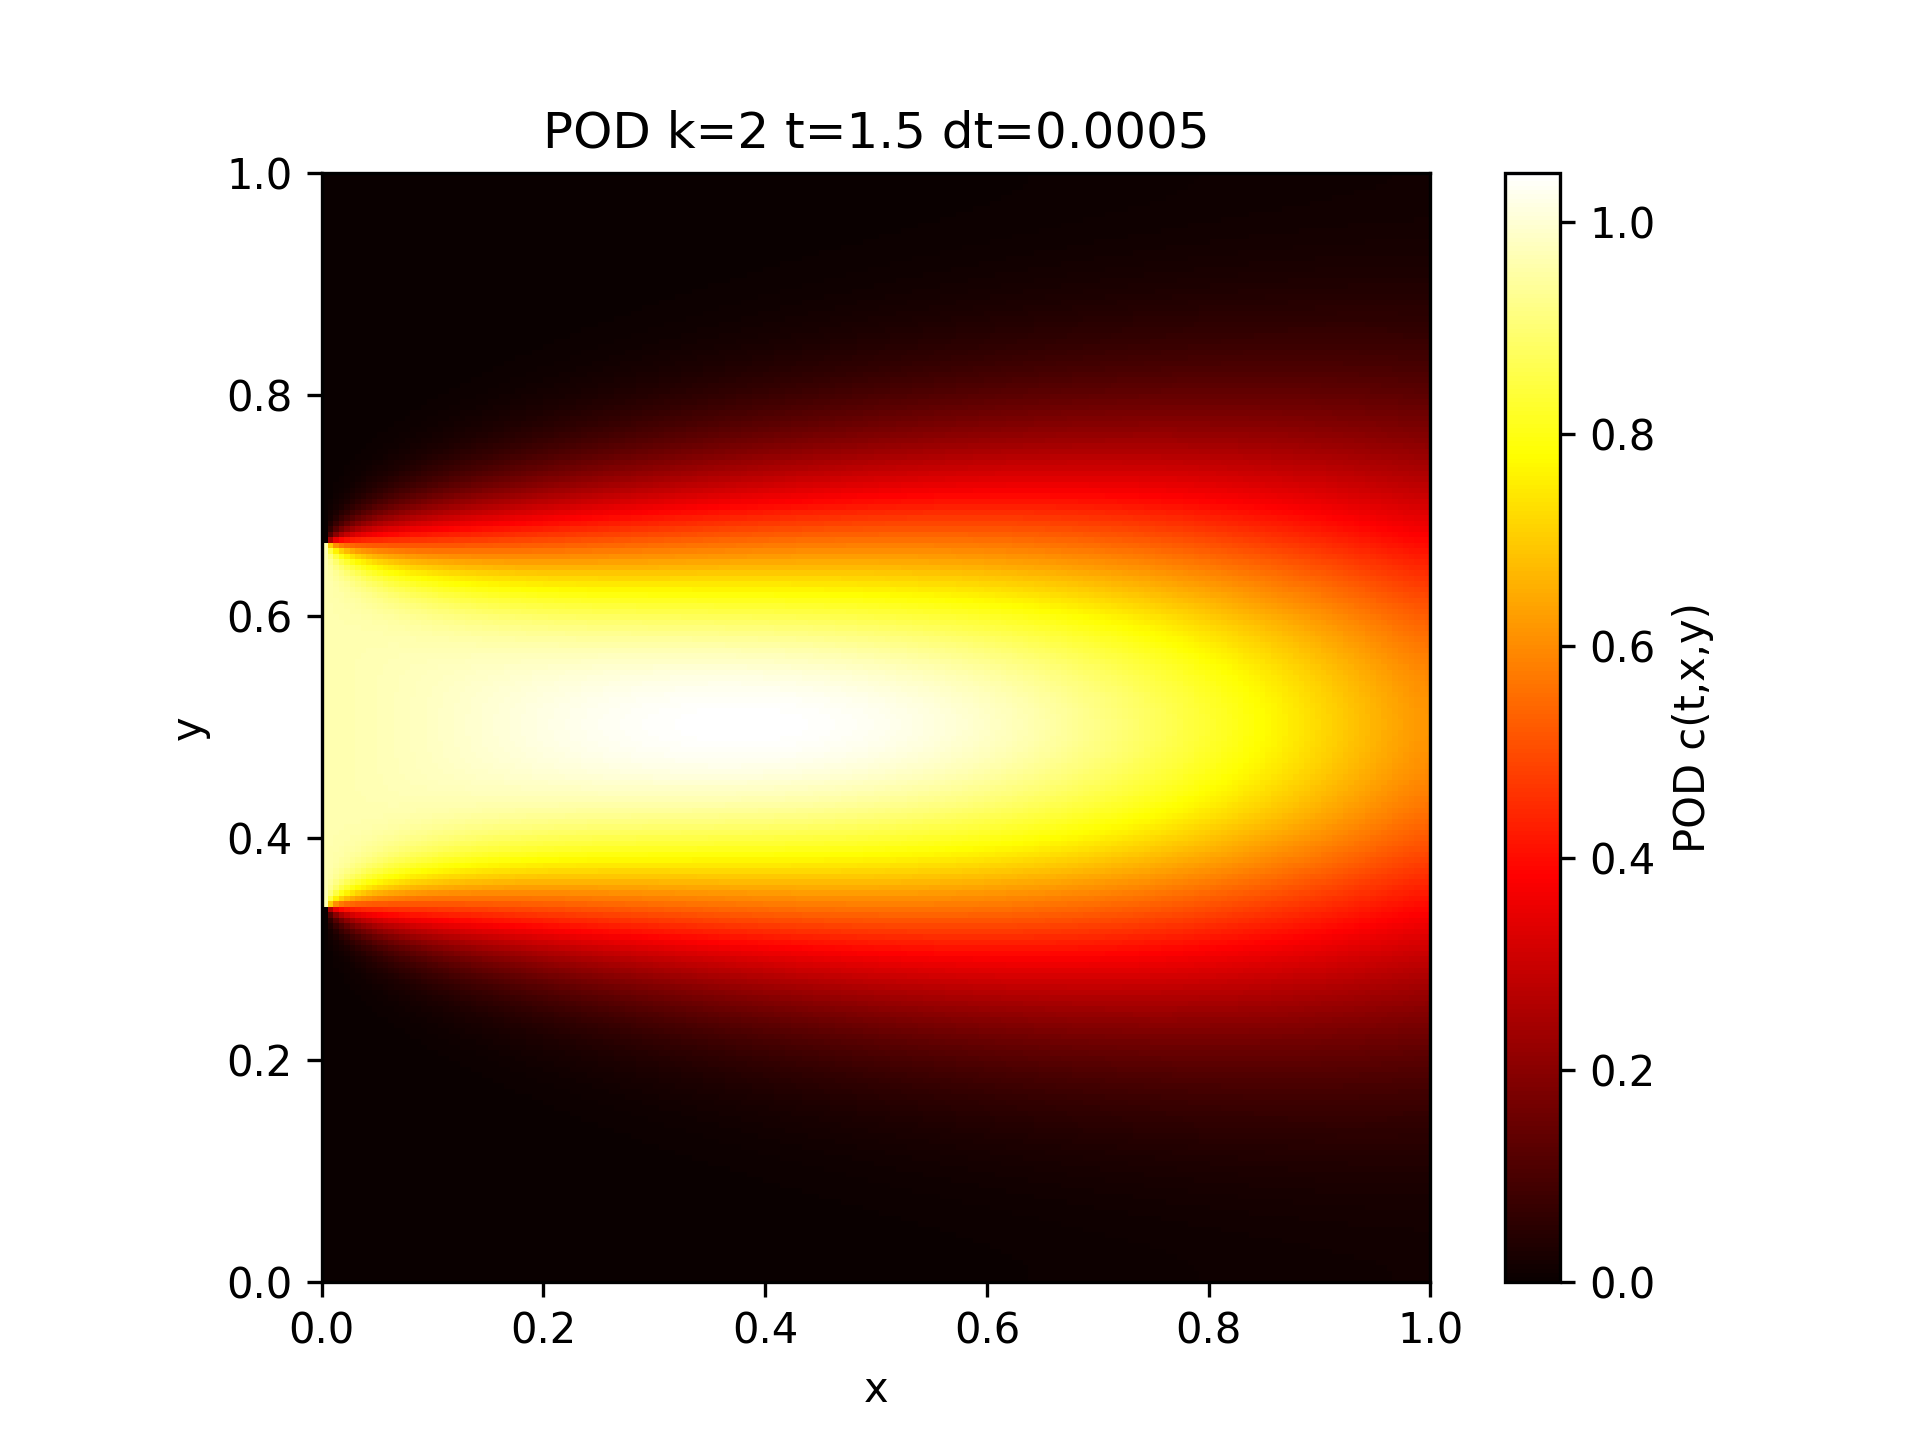
\includegraphics[width=\textwidth]{POD k=2 t=1.5 dt=0.0005.png}
        \caption{POD k=2 t=1.5 dt=0.0005}
        \label{POD k=2 t=1.5 dt=0.0005}
    \end{subfigure}
    
    \caption{results of POD k = 2}
    \label{results of POD k = 2}
\end{figure}

\begin{figure}[htbp]
    \centering
    % 2x2 排列
    \begin{subfigure}{0.45\textwidth}
        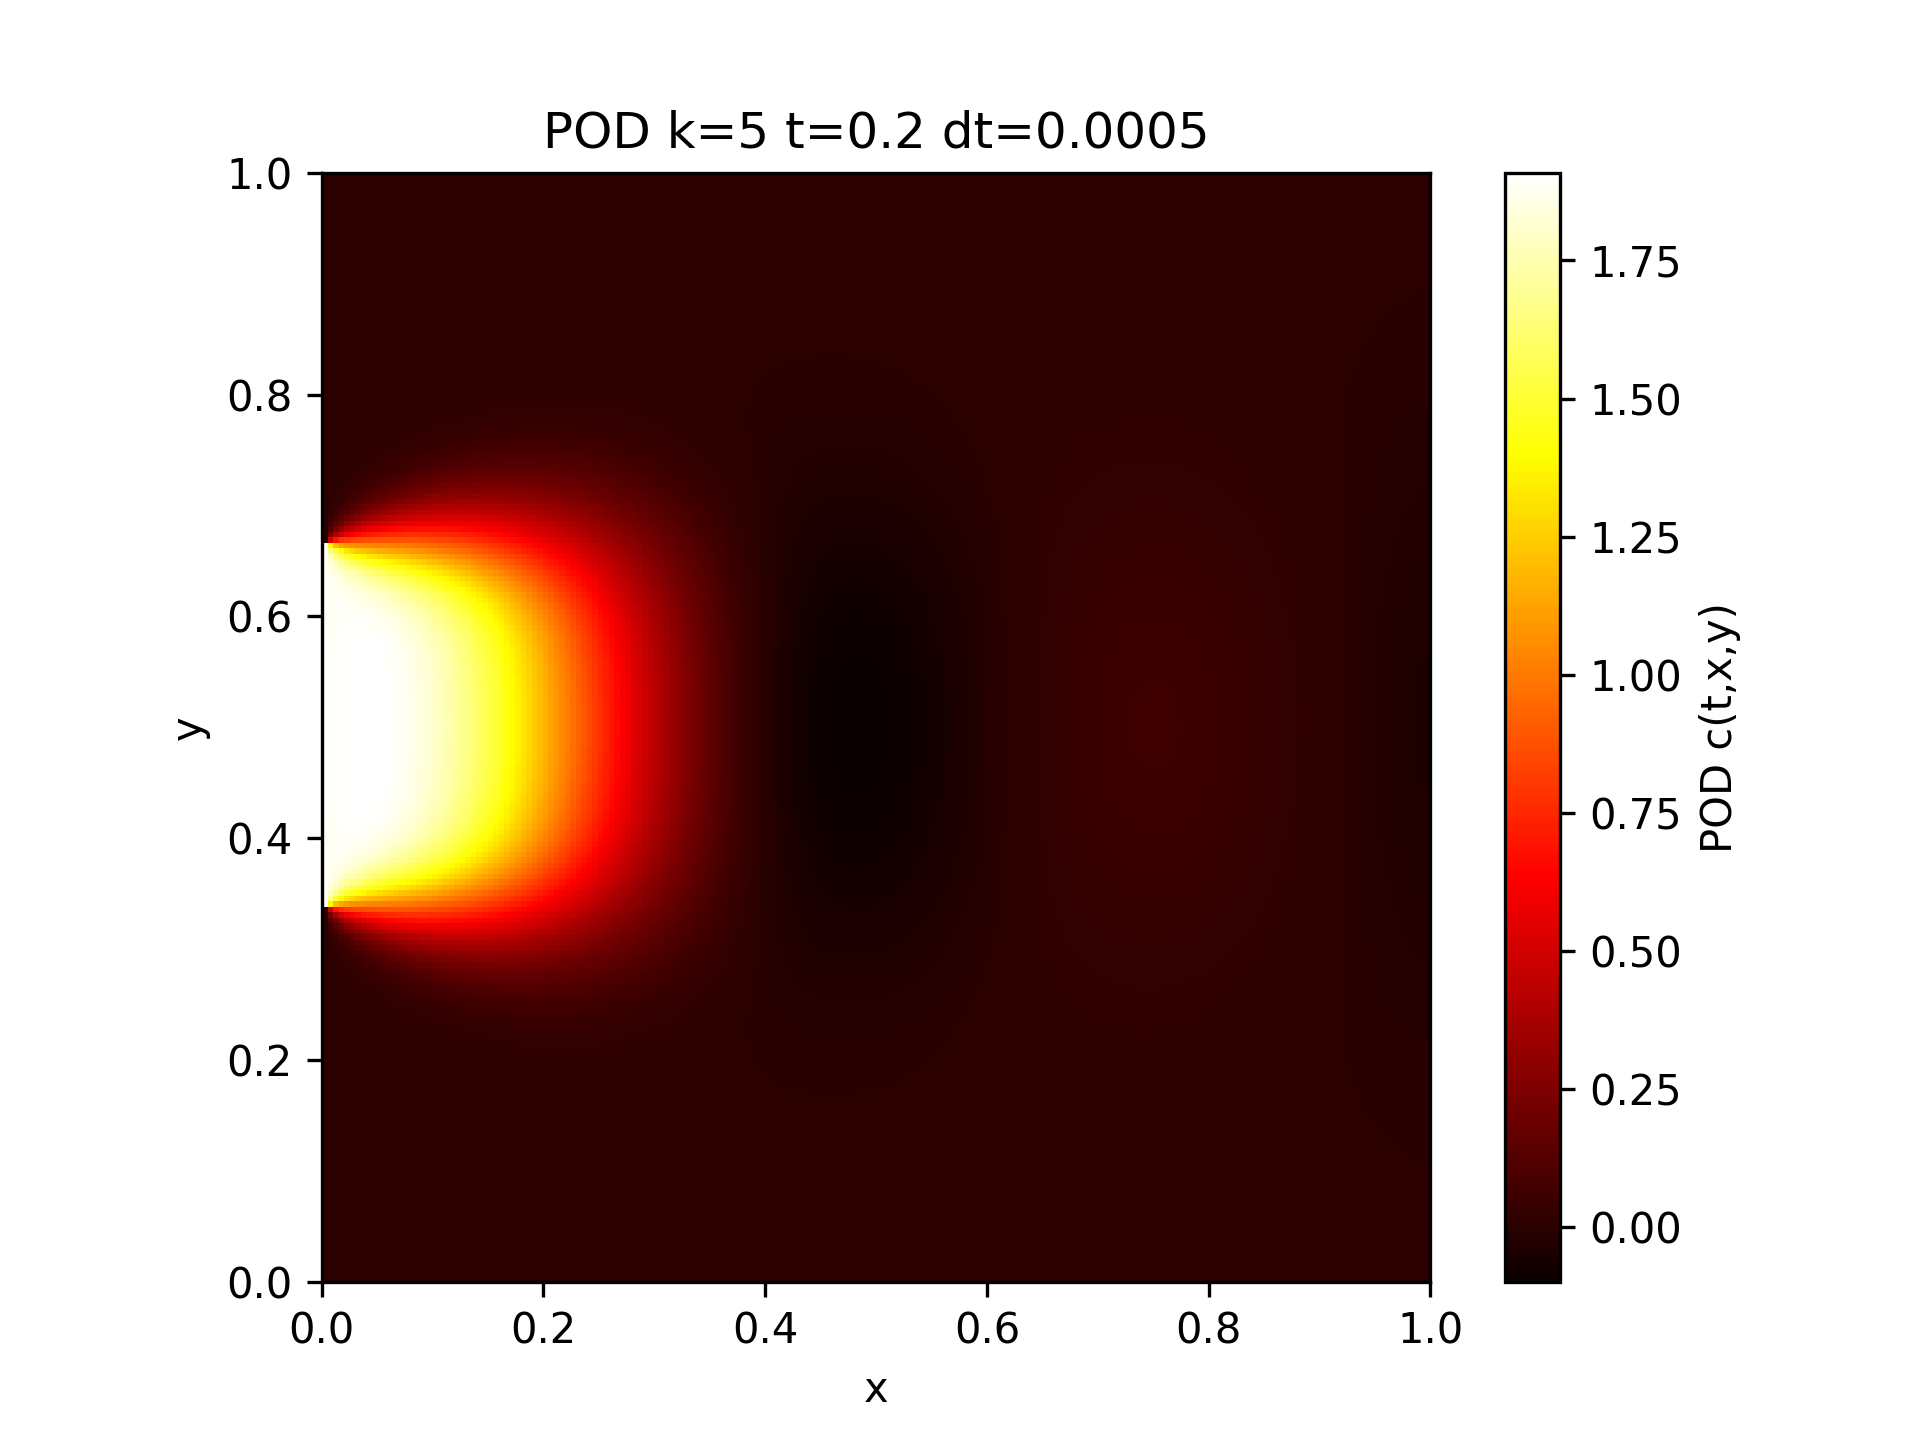
\includegraphics[width=\textwidth]{POD k=5 t=0.2 dt=0.0005.png}
        \caption{POD k=5 t=0.2 dt=0.0005}
        \label{POD k=5 t=0.2 dt=0.0005}
    \end{subfigure}
    \hfill
    \begin{subfigure}{0.45\textwidth}
        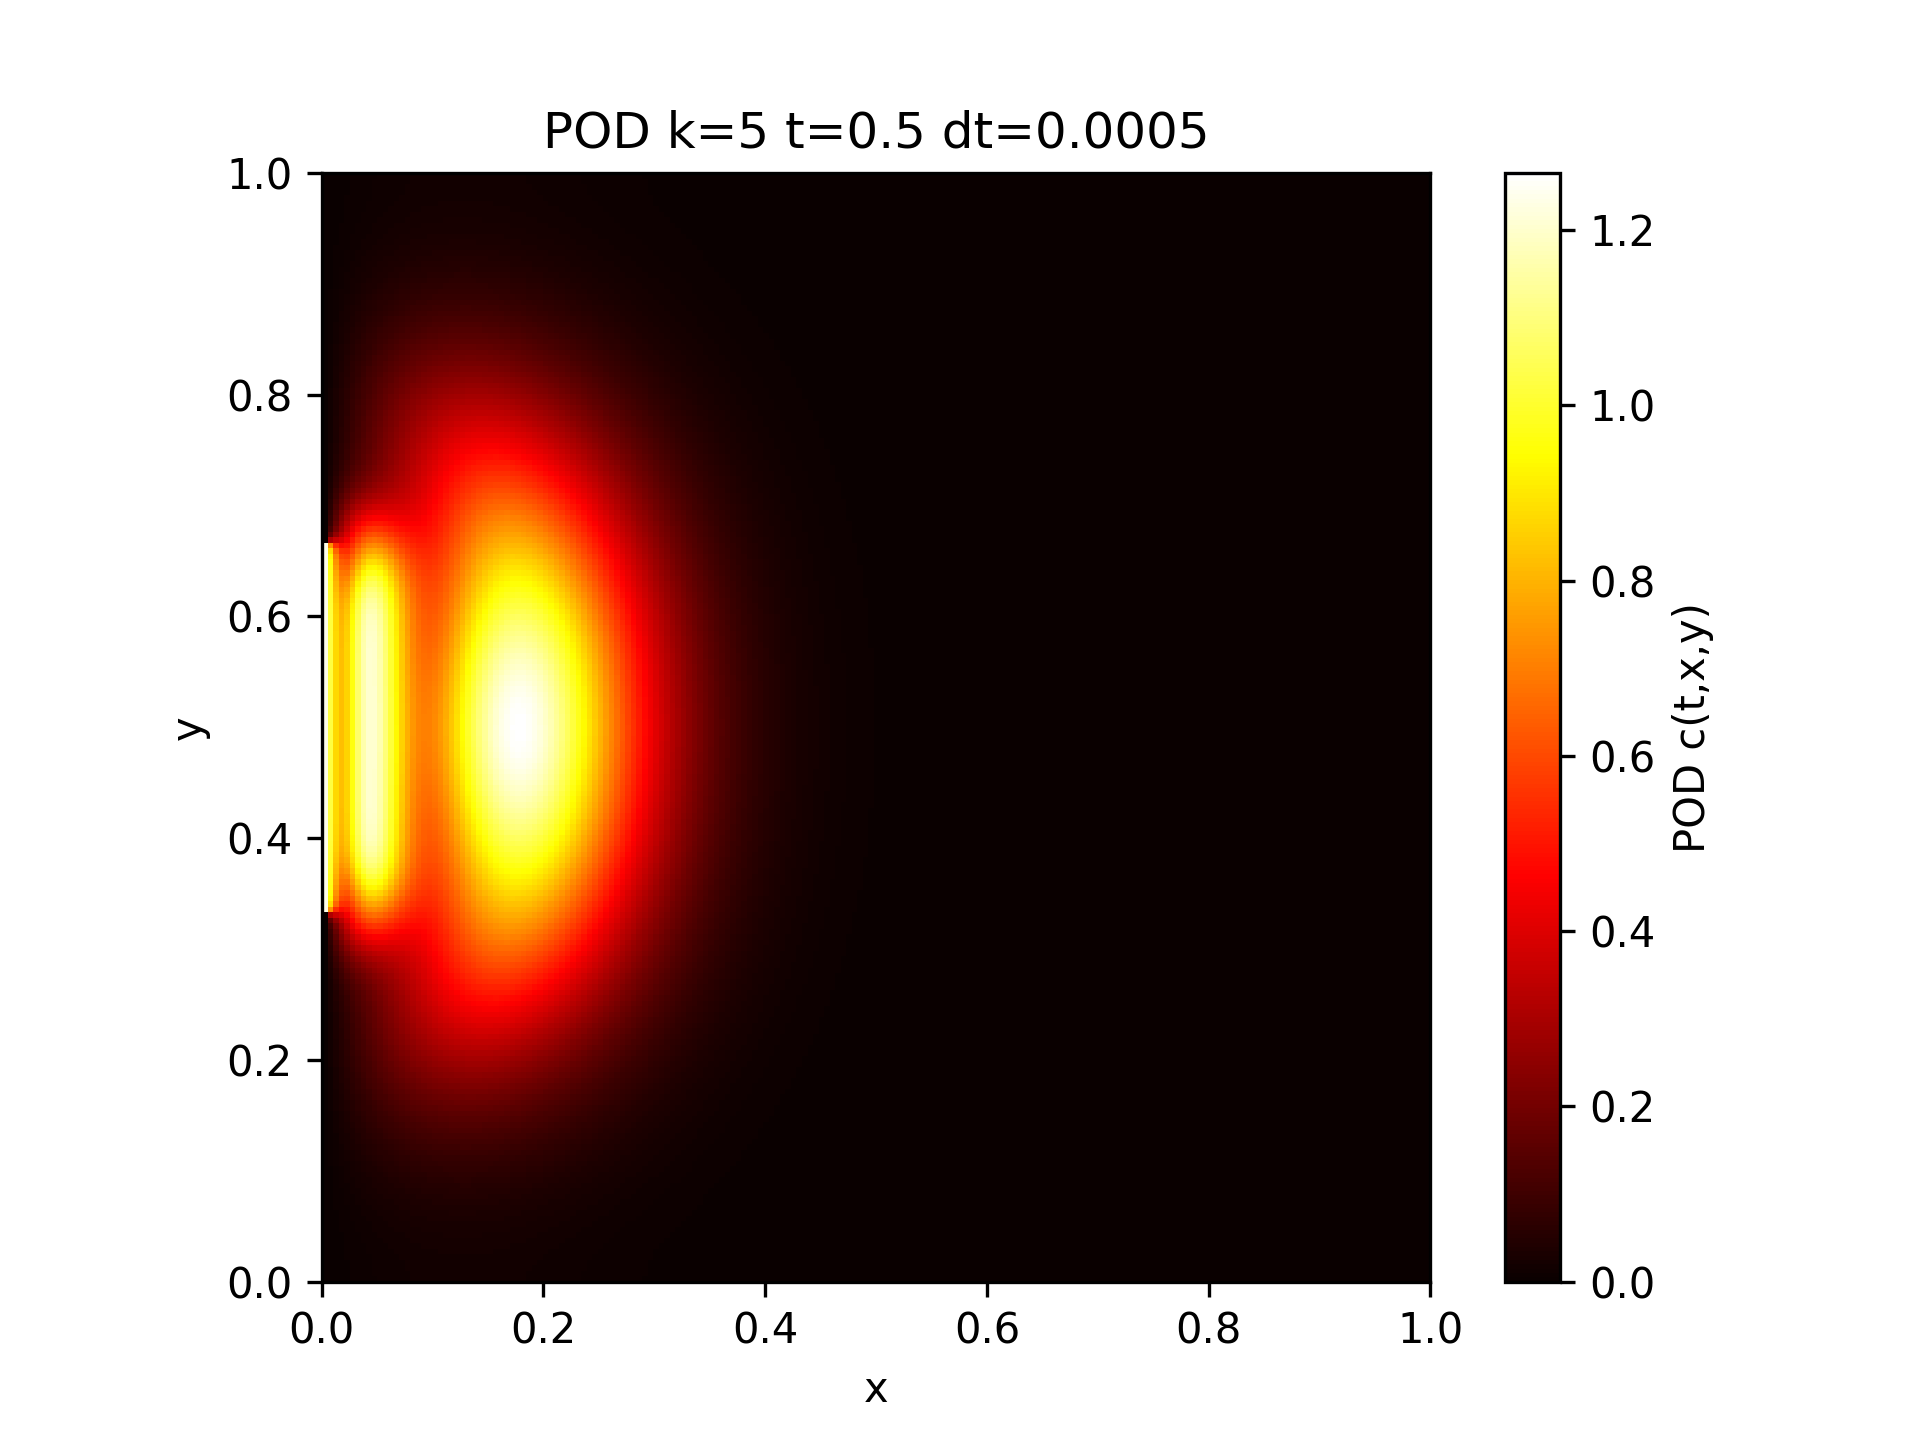
\includegraphics[width=\textwidth]{POD k=5 t=0.5 dt=0.0005.png}
        \caption{POD k=5 t=0.5 dt=0.0005}
        \label{POD k=5 t=0.5 dt=0.0005}
    \end{subfigure}
    
    \vspace{0.5cm}  % 垂直间距
    
    \begin{subfigure}{0.45\textwidth}
        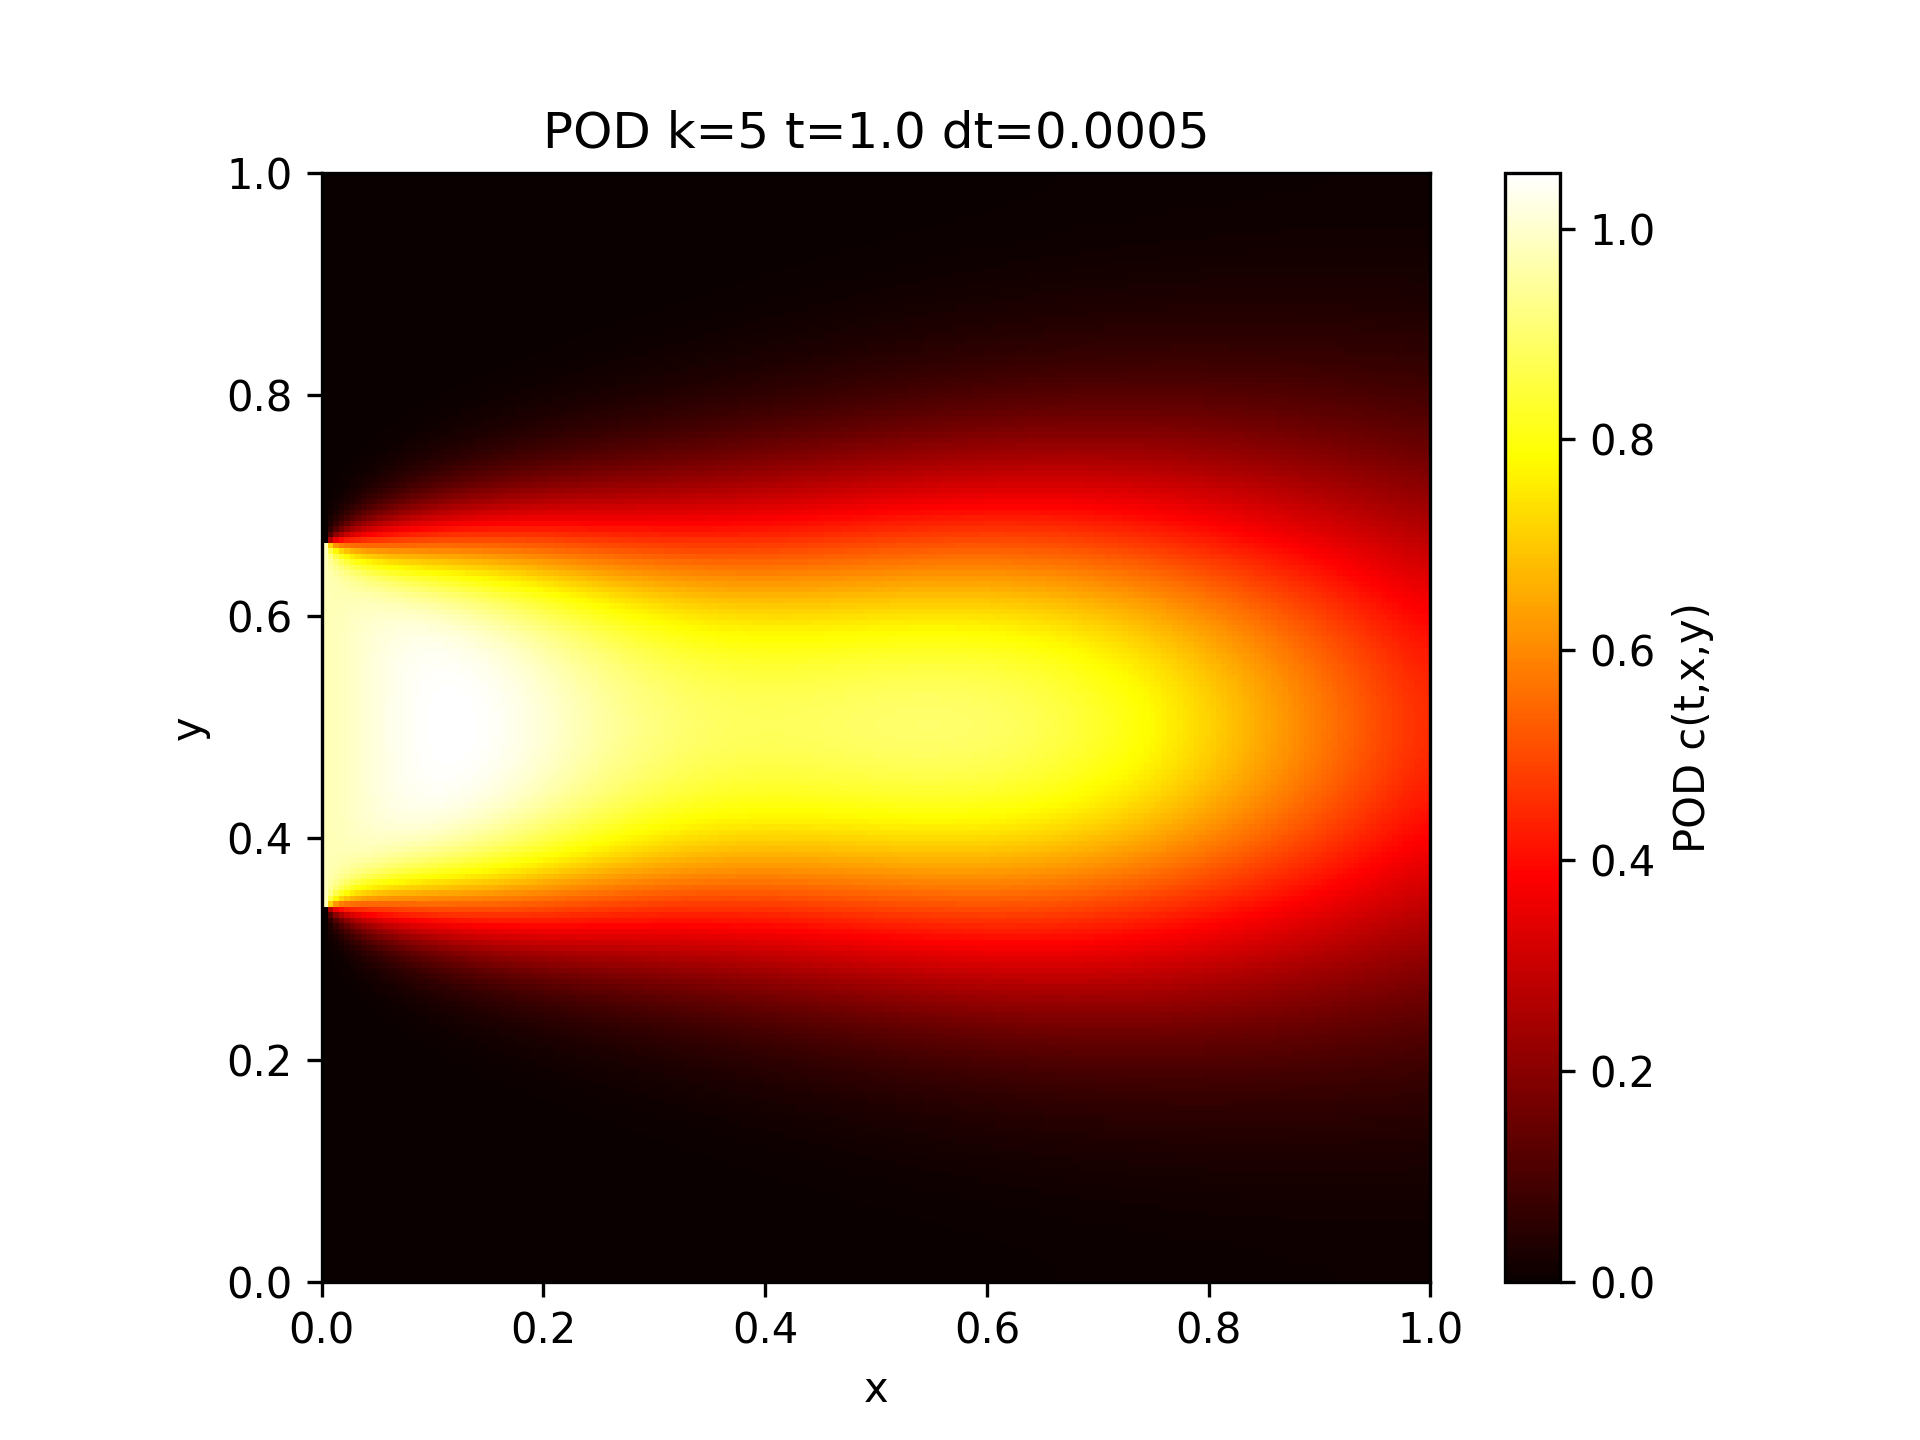
\includegraphics[width=\textwidth]{POD k=5 t=1.0 dt=0.0005.png}
        \caption{POD k=5 t=1.0 dt=0.0005}
        \label{POD k=5 t=1.0 dt=0.0005}
    \end{subfigure}
    \hfill
    \begin{subfigure}{0.45\textwidth}
        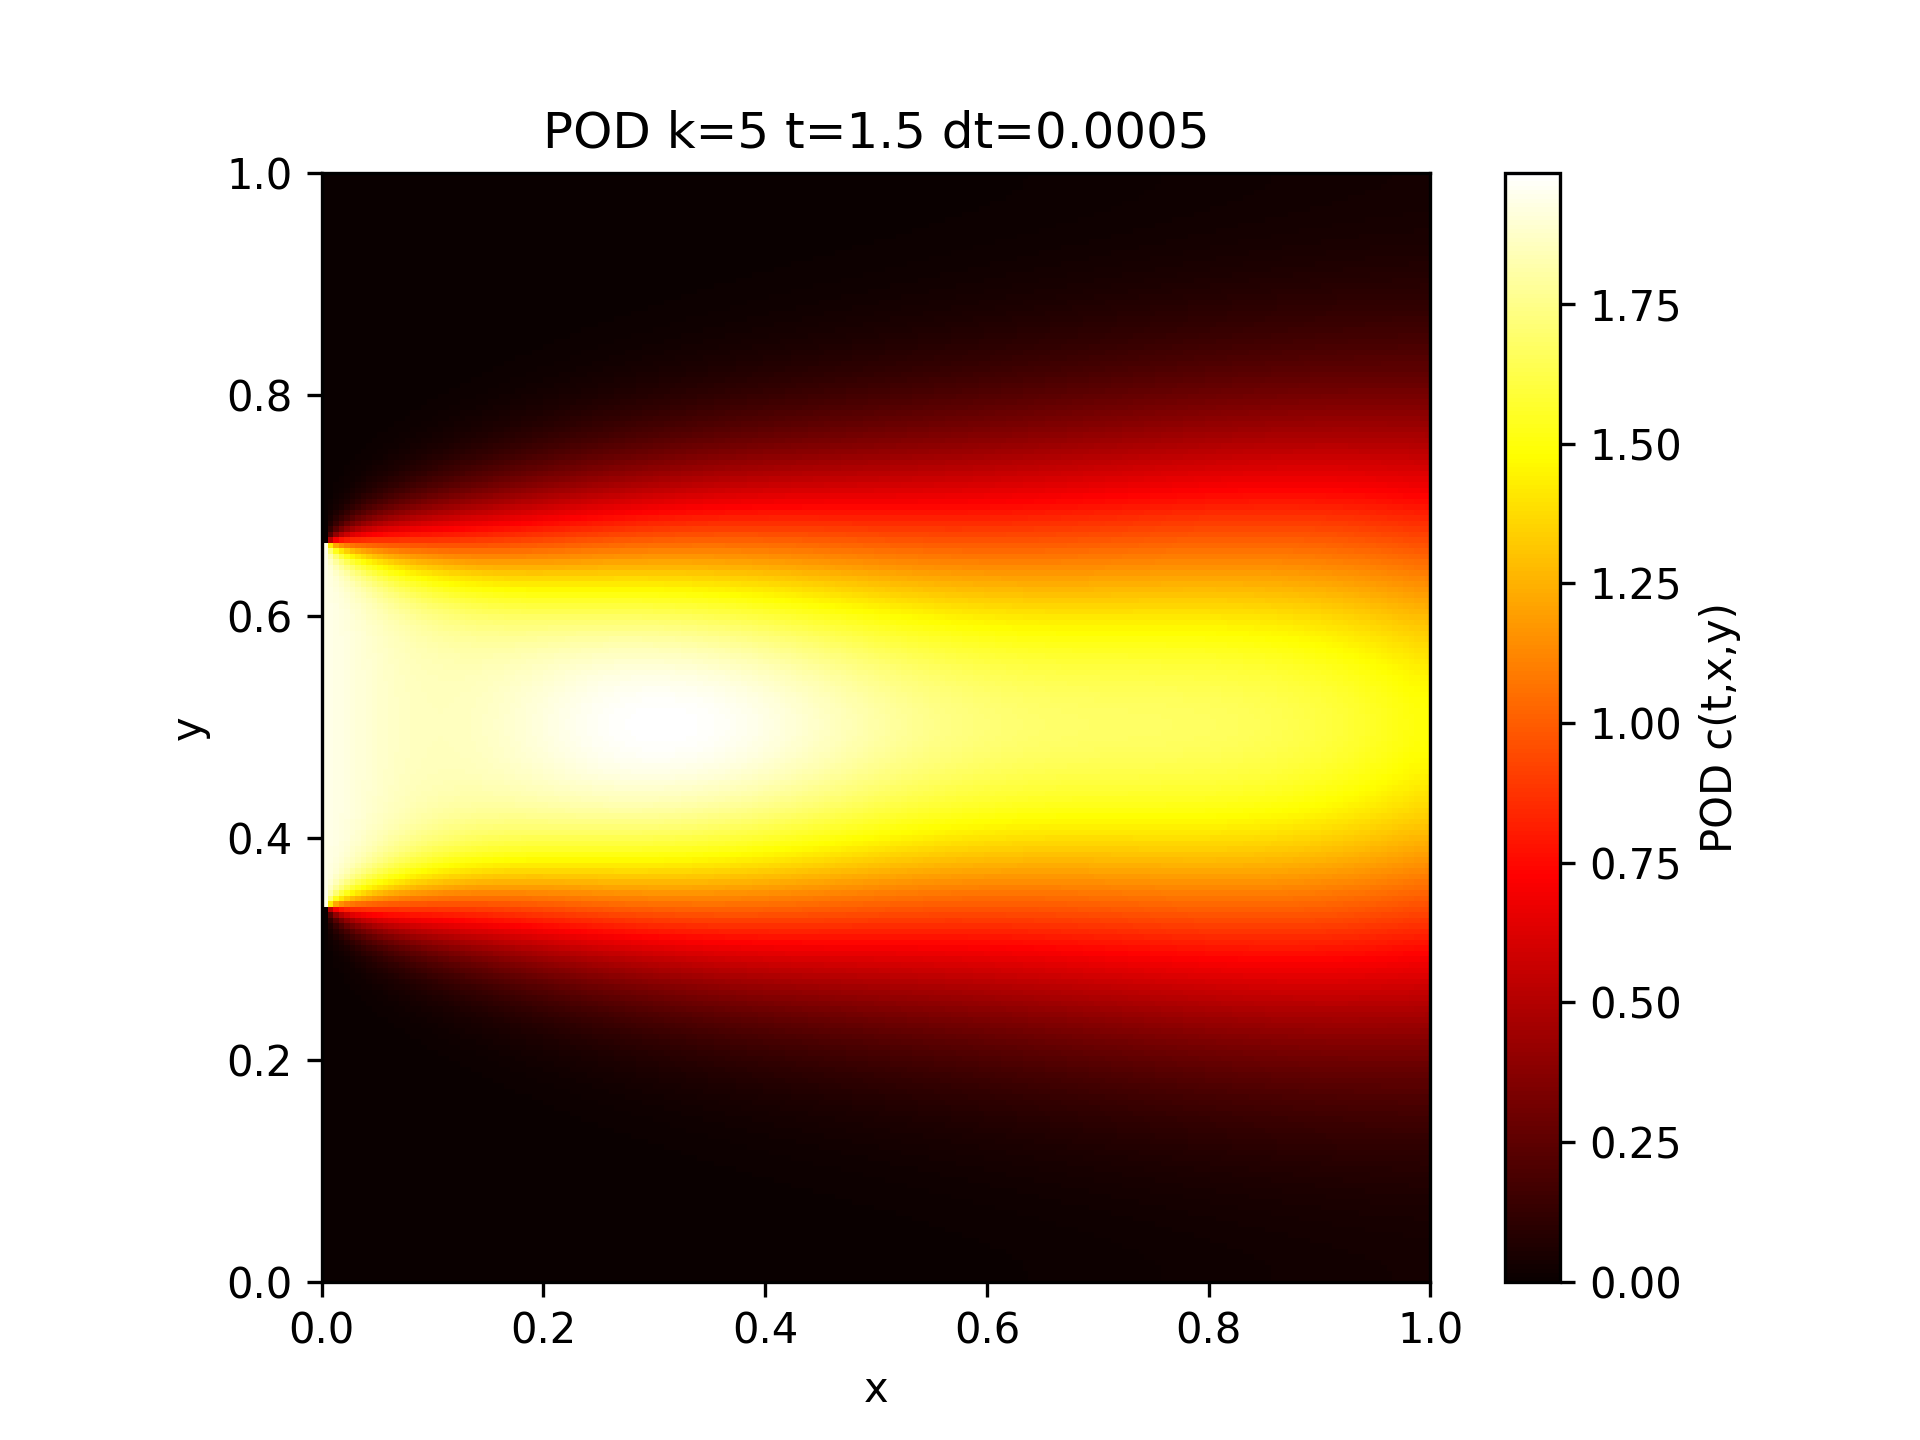
\includegraphics[width=\textwidth]{POD k=5 t=1.5 dt=0.0005.png}
        \caption{POD k=5 t=1.5 dt=0.0005}
        \label{POD k=5 t=1.5 dt=0.0005}
    \end{subfigure}
    
    \caption{results of POD k = 5}
    \label{results of POD k = 5}
\end{figure}

\begin{figure}[htbp]
    \centering
    % 2x2 排列
    \begin{subfigure}{0.45\textwidth}
        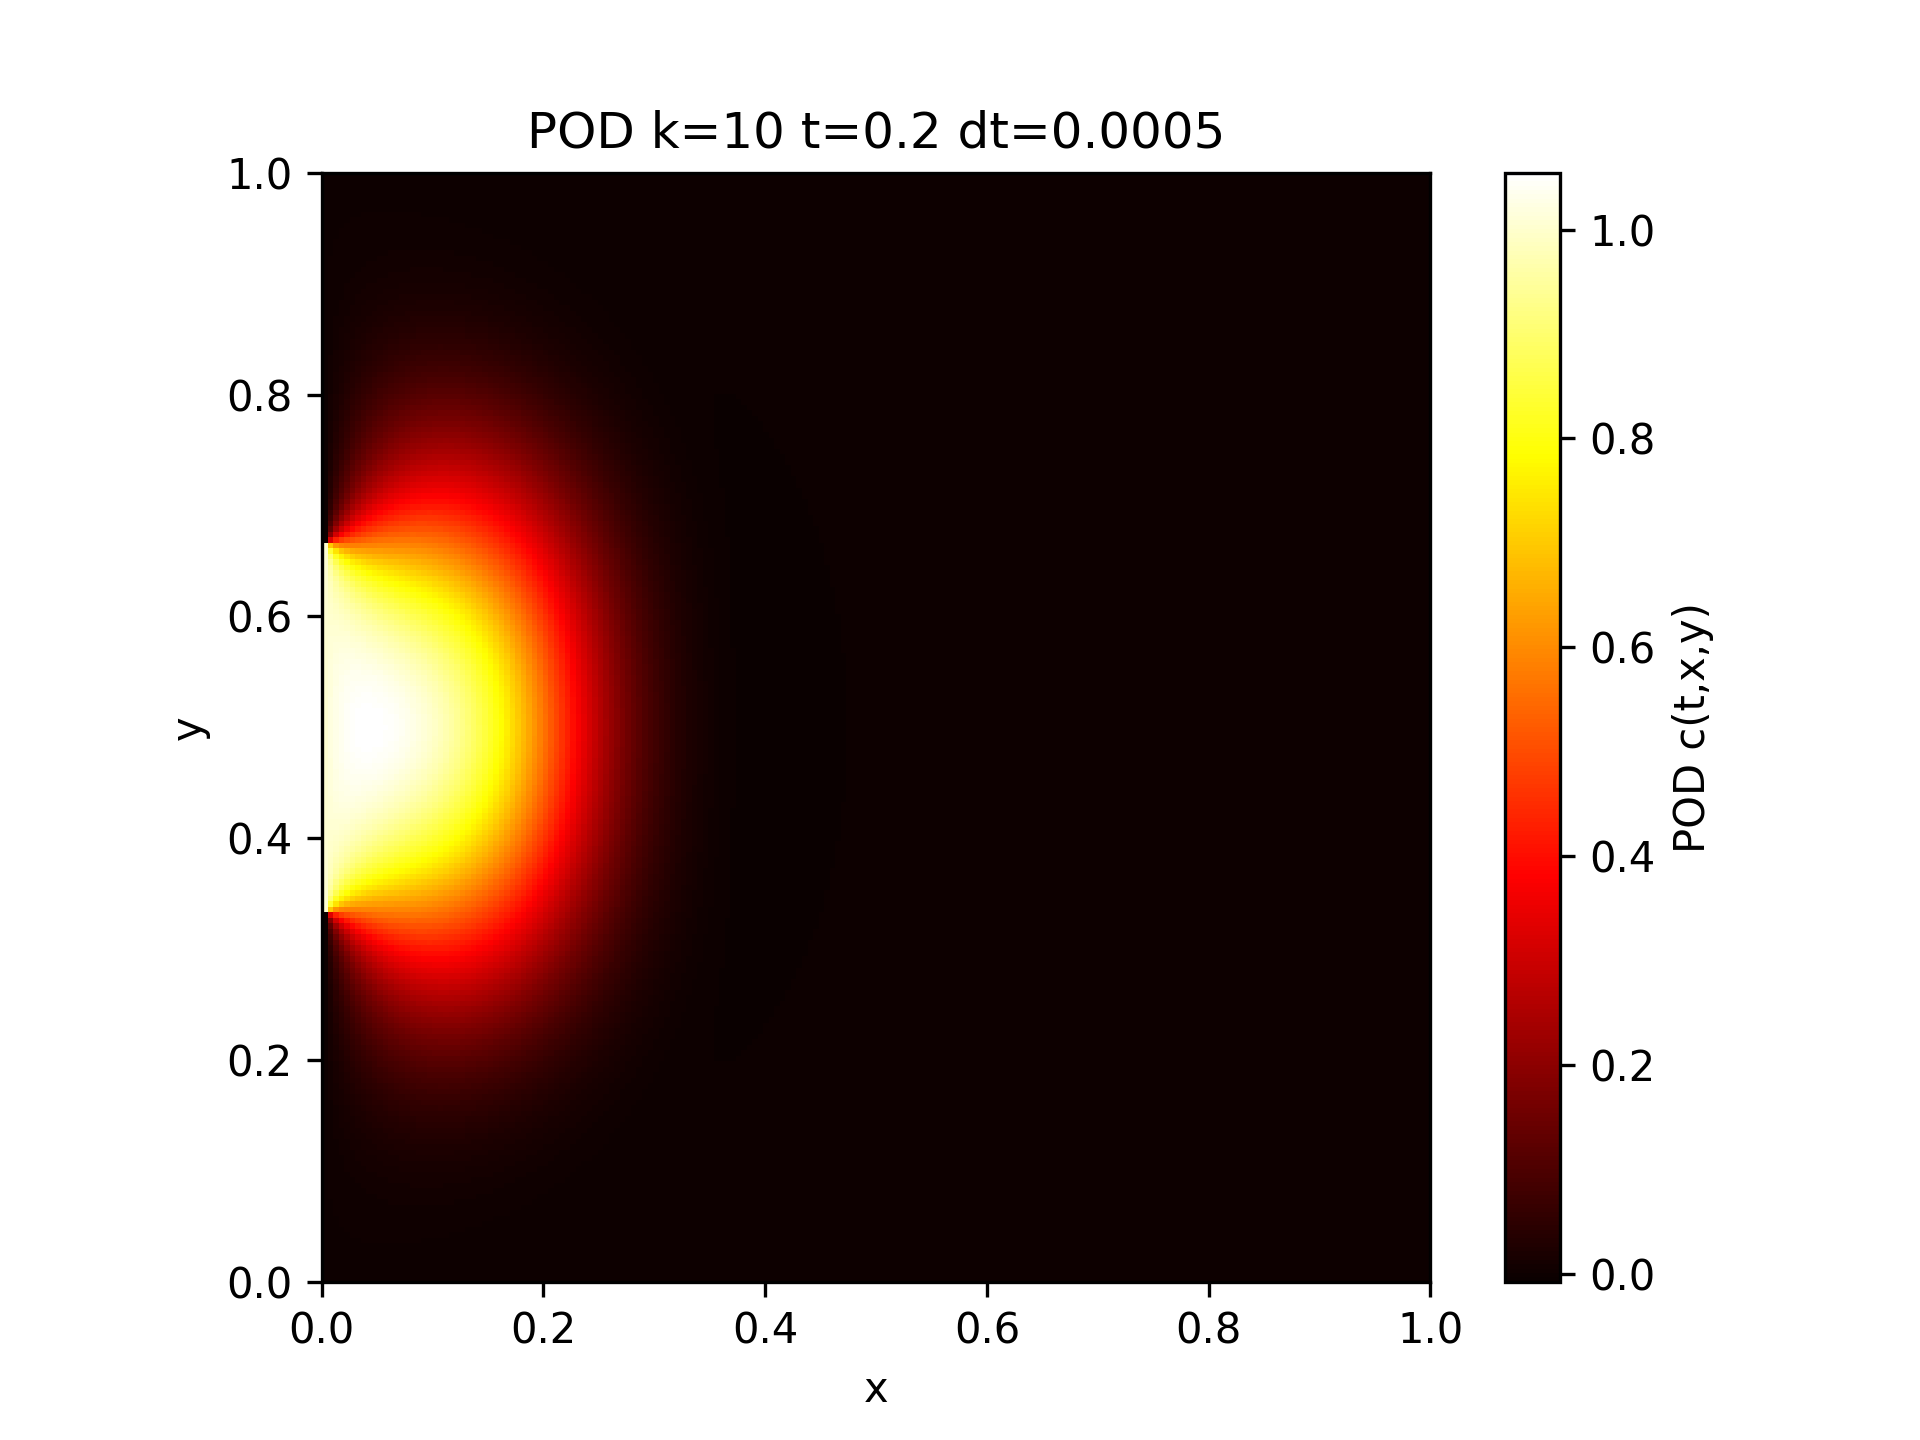
\includegraphics[width=\textwidth]{POD k=10 t=0.2 dt=0.0005.png}
        \caption{POD k=10 t=0.2 dt=0.0005}
        \label{POD k=10 t=0.2 dt=0.0005}
    \end{subfigure}
    \hfill
    \begin{subfigure}{0.45\textwidth}
        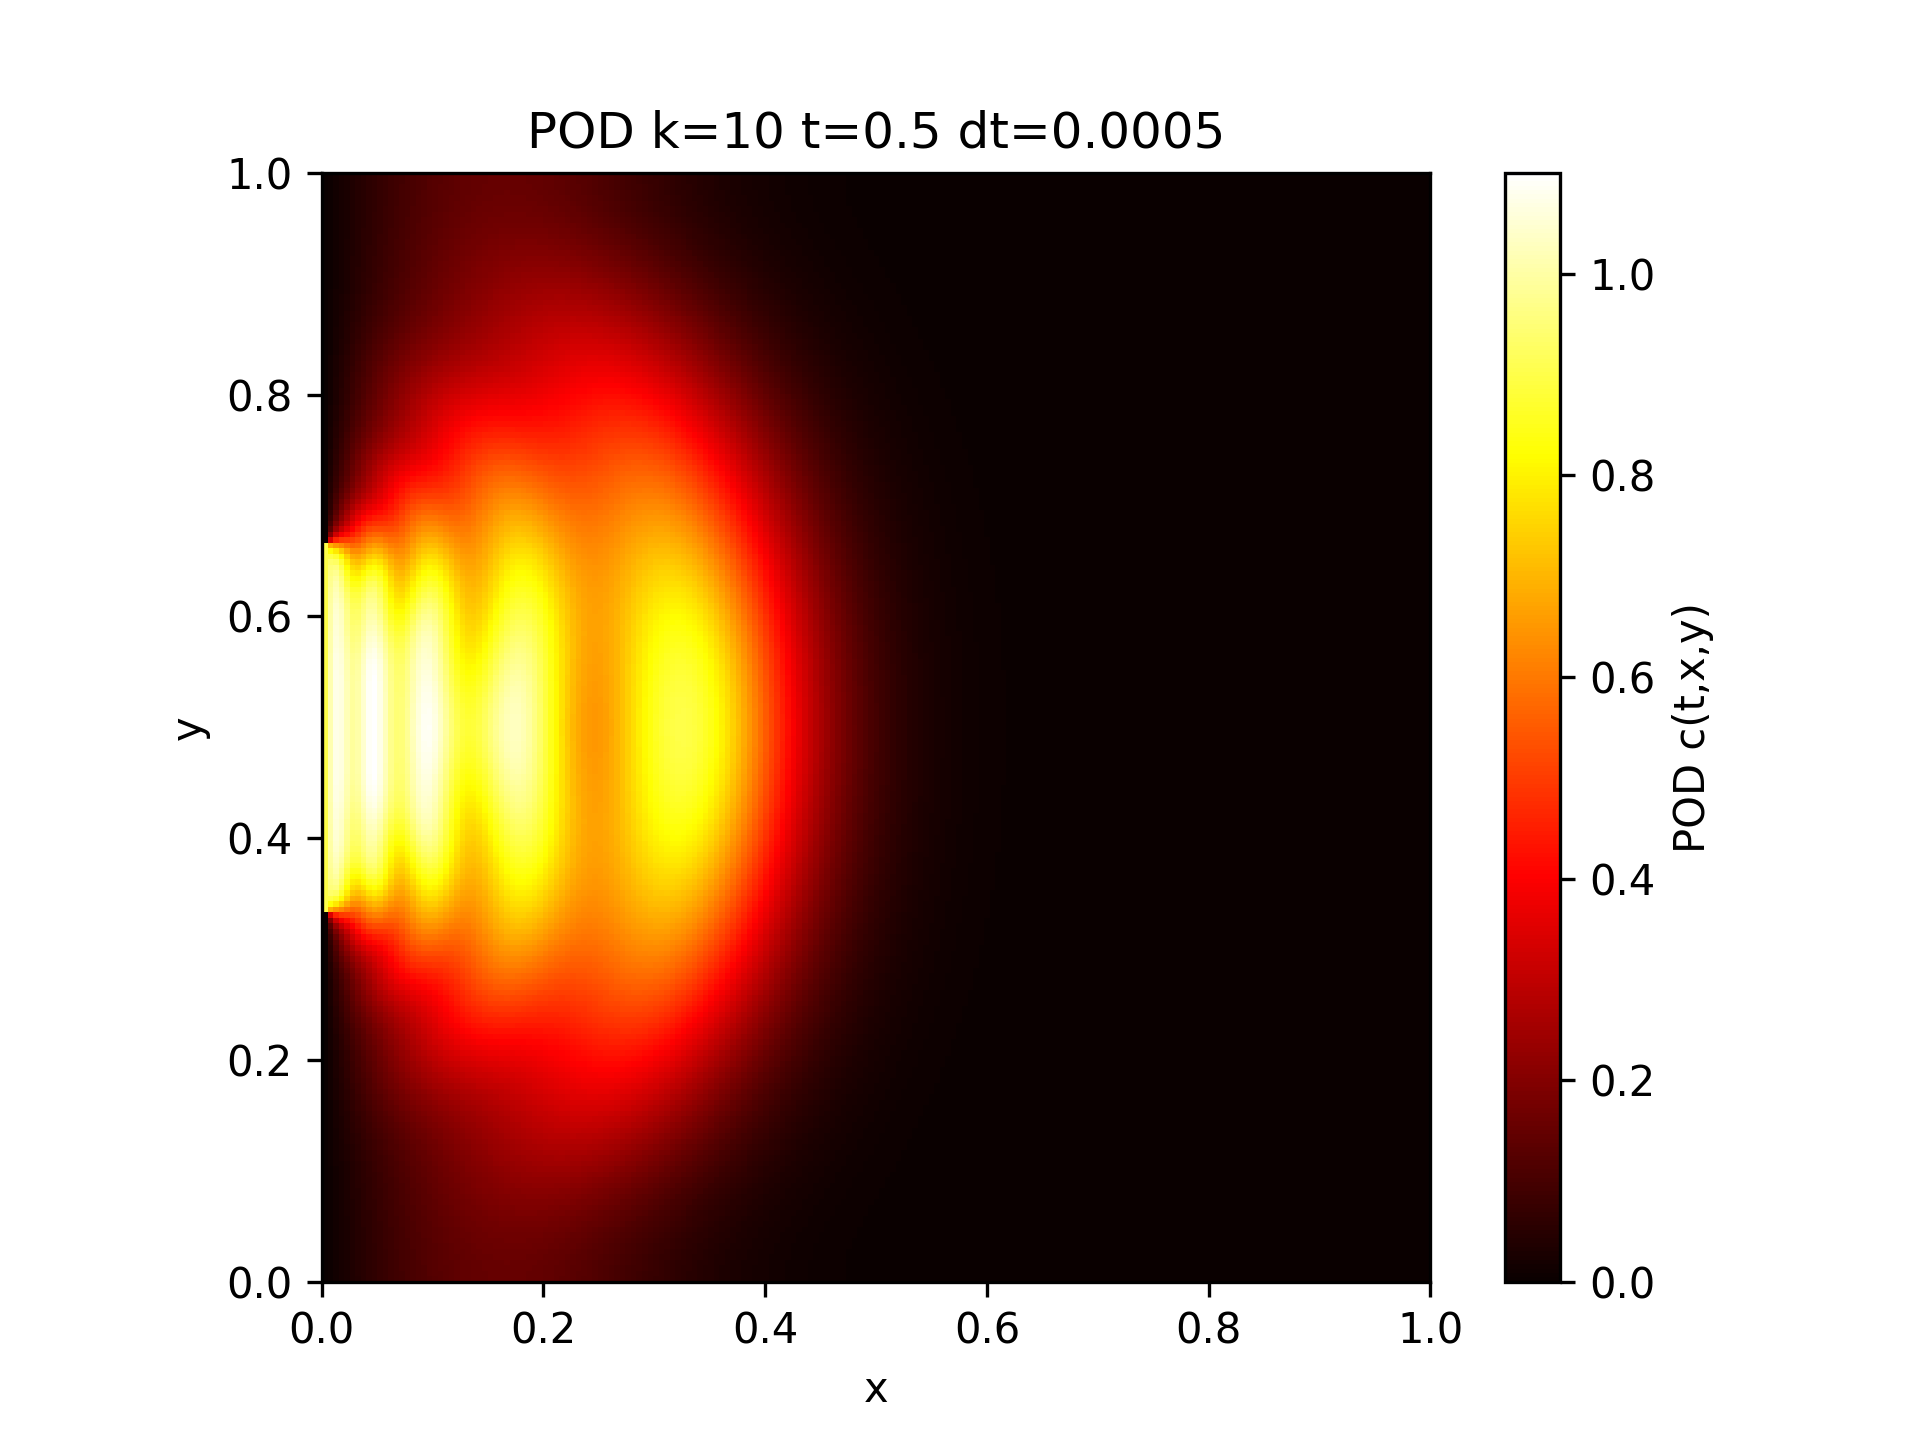
\includegraphics[width=\textwidth]{POD k=10 t=0.5 dt=0.0005.png}
        \caption{POD k=10 t=0.5 dt=0.0005}
        \label{POD k=10 t=0.5 dt=0.0005}
    \end{subfigure}
    
    \vspace{0.5cm}  % 垂直间距
    
    \begin{subfigure}{0.45\textwidth}
        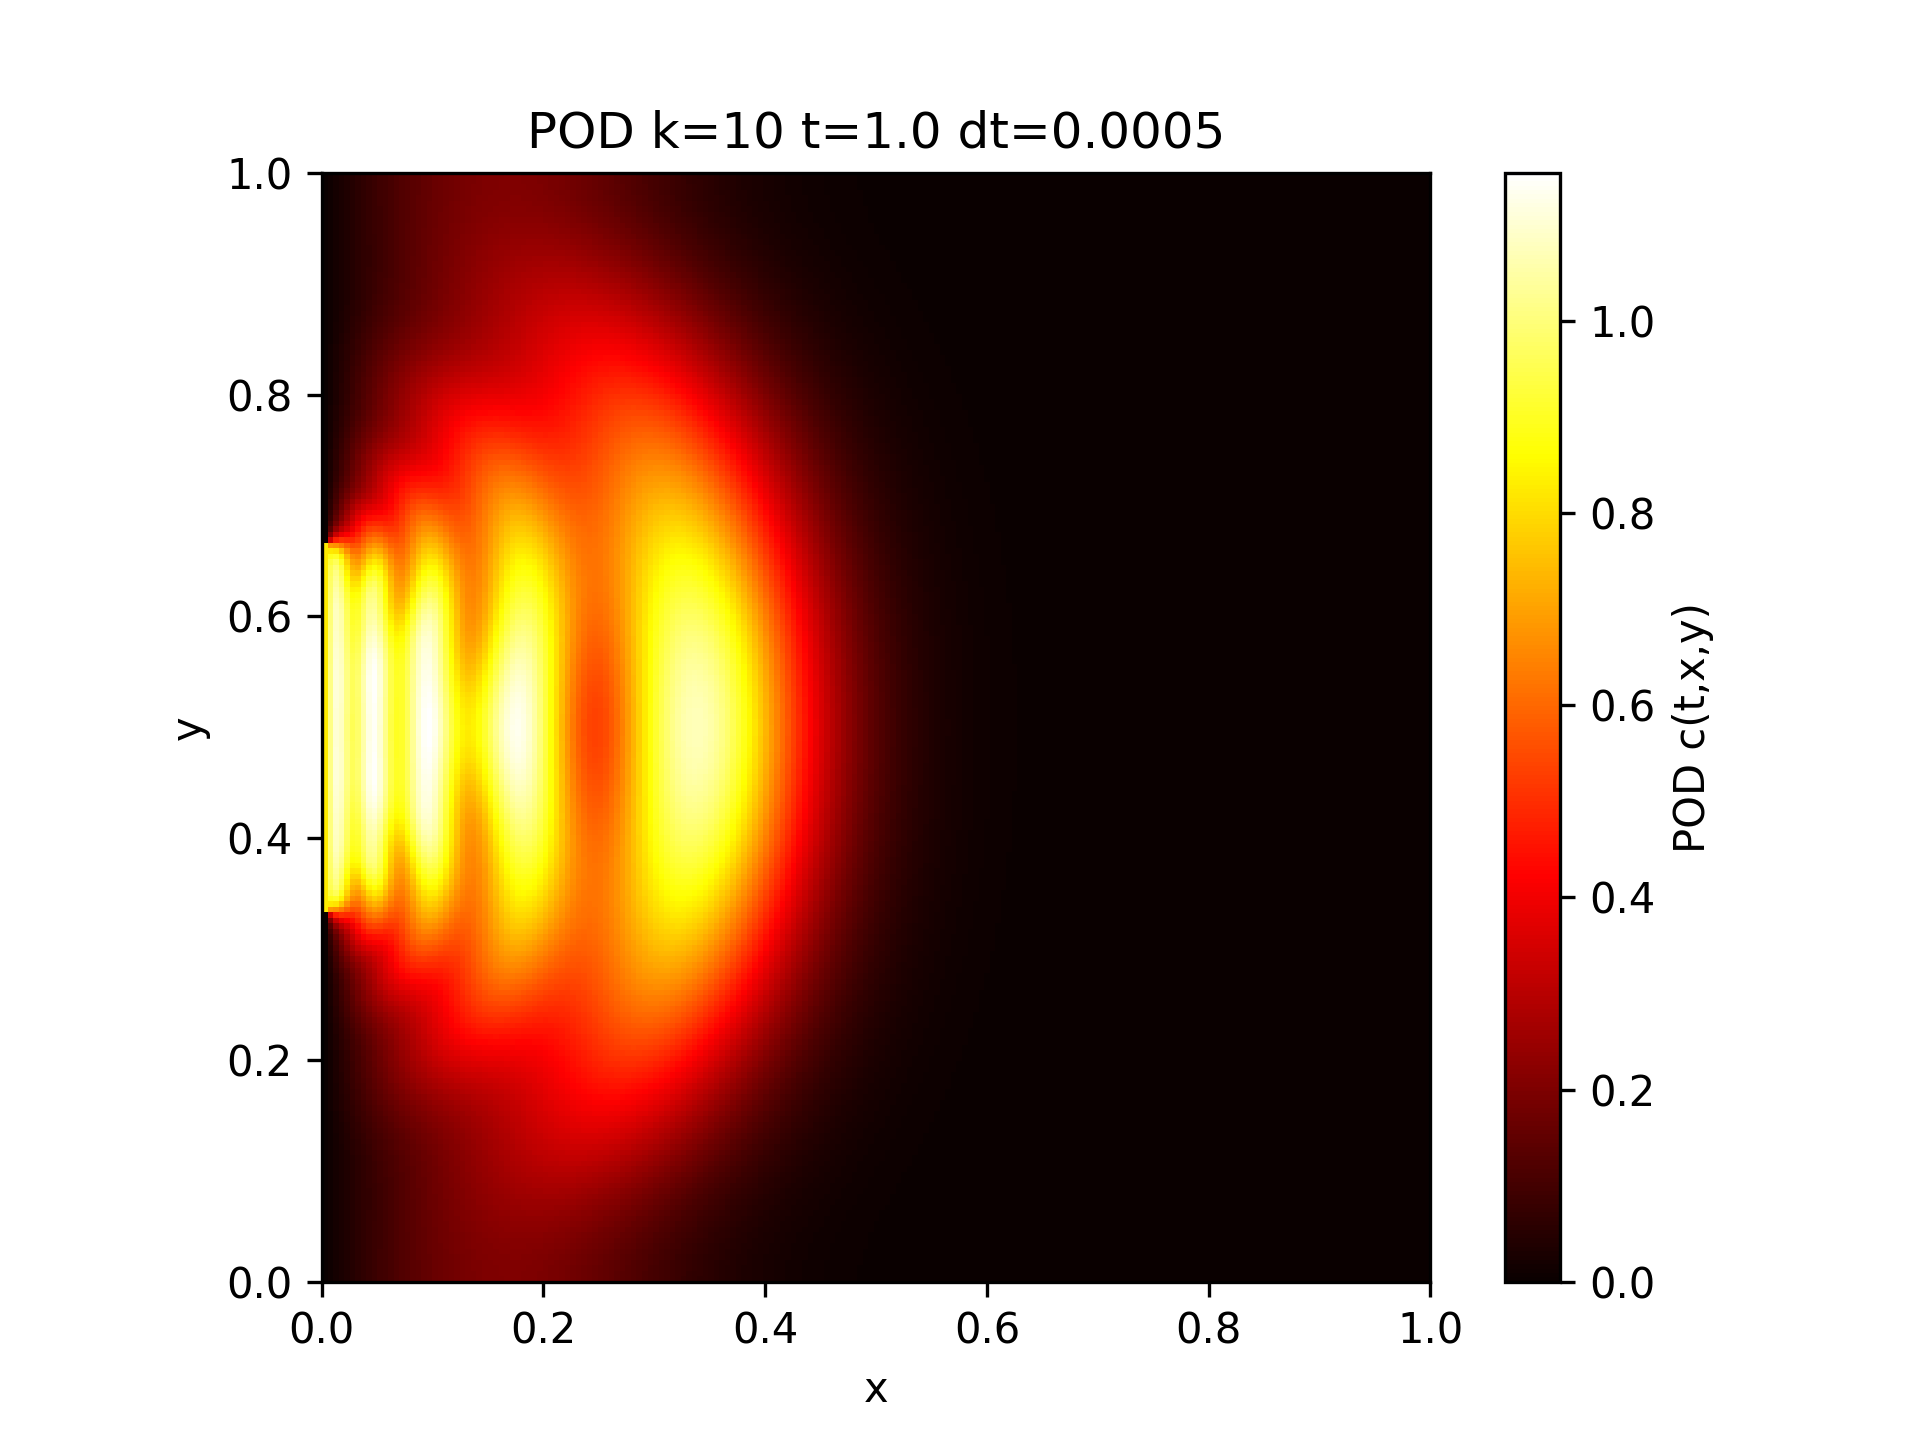
\includegraphics[width=\textwidth]{POD k=10 t=1.0 dt=0.0005.png}
        \caption{POD k=10 t=1.0 dt=0.0005}
        \label{POD k=10 t=1.0 dt=0.0005}
    \end{subfigure}
    \hfill
    \begin{subfigure}{0.45\textwidth}
        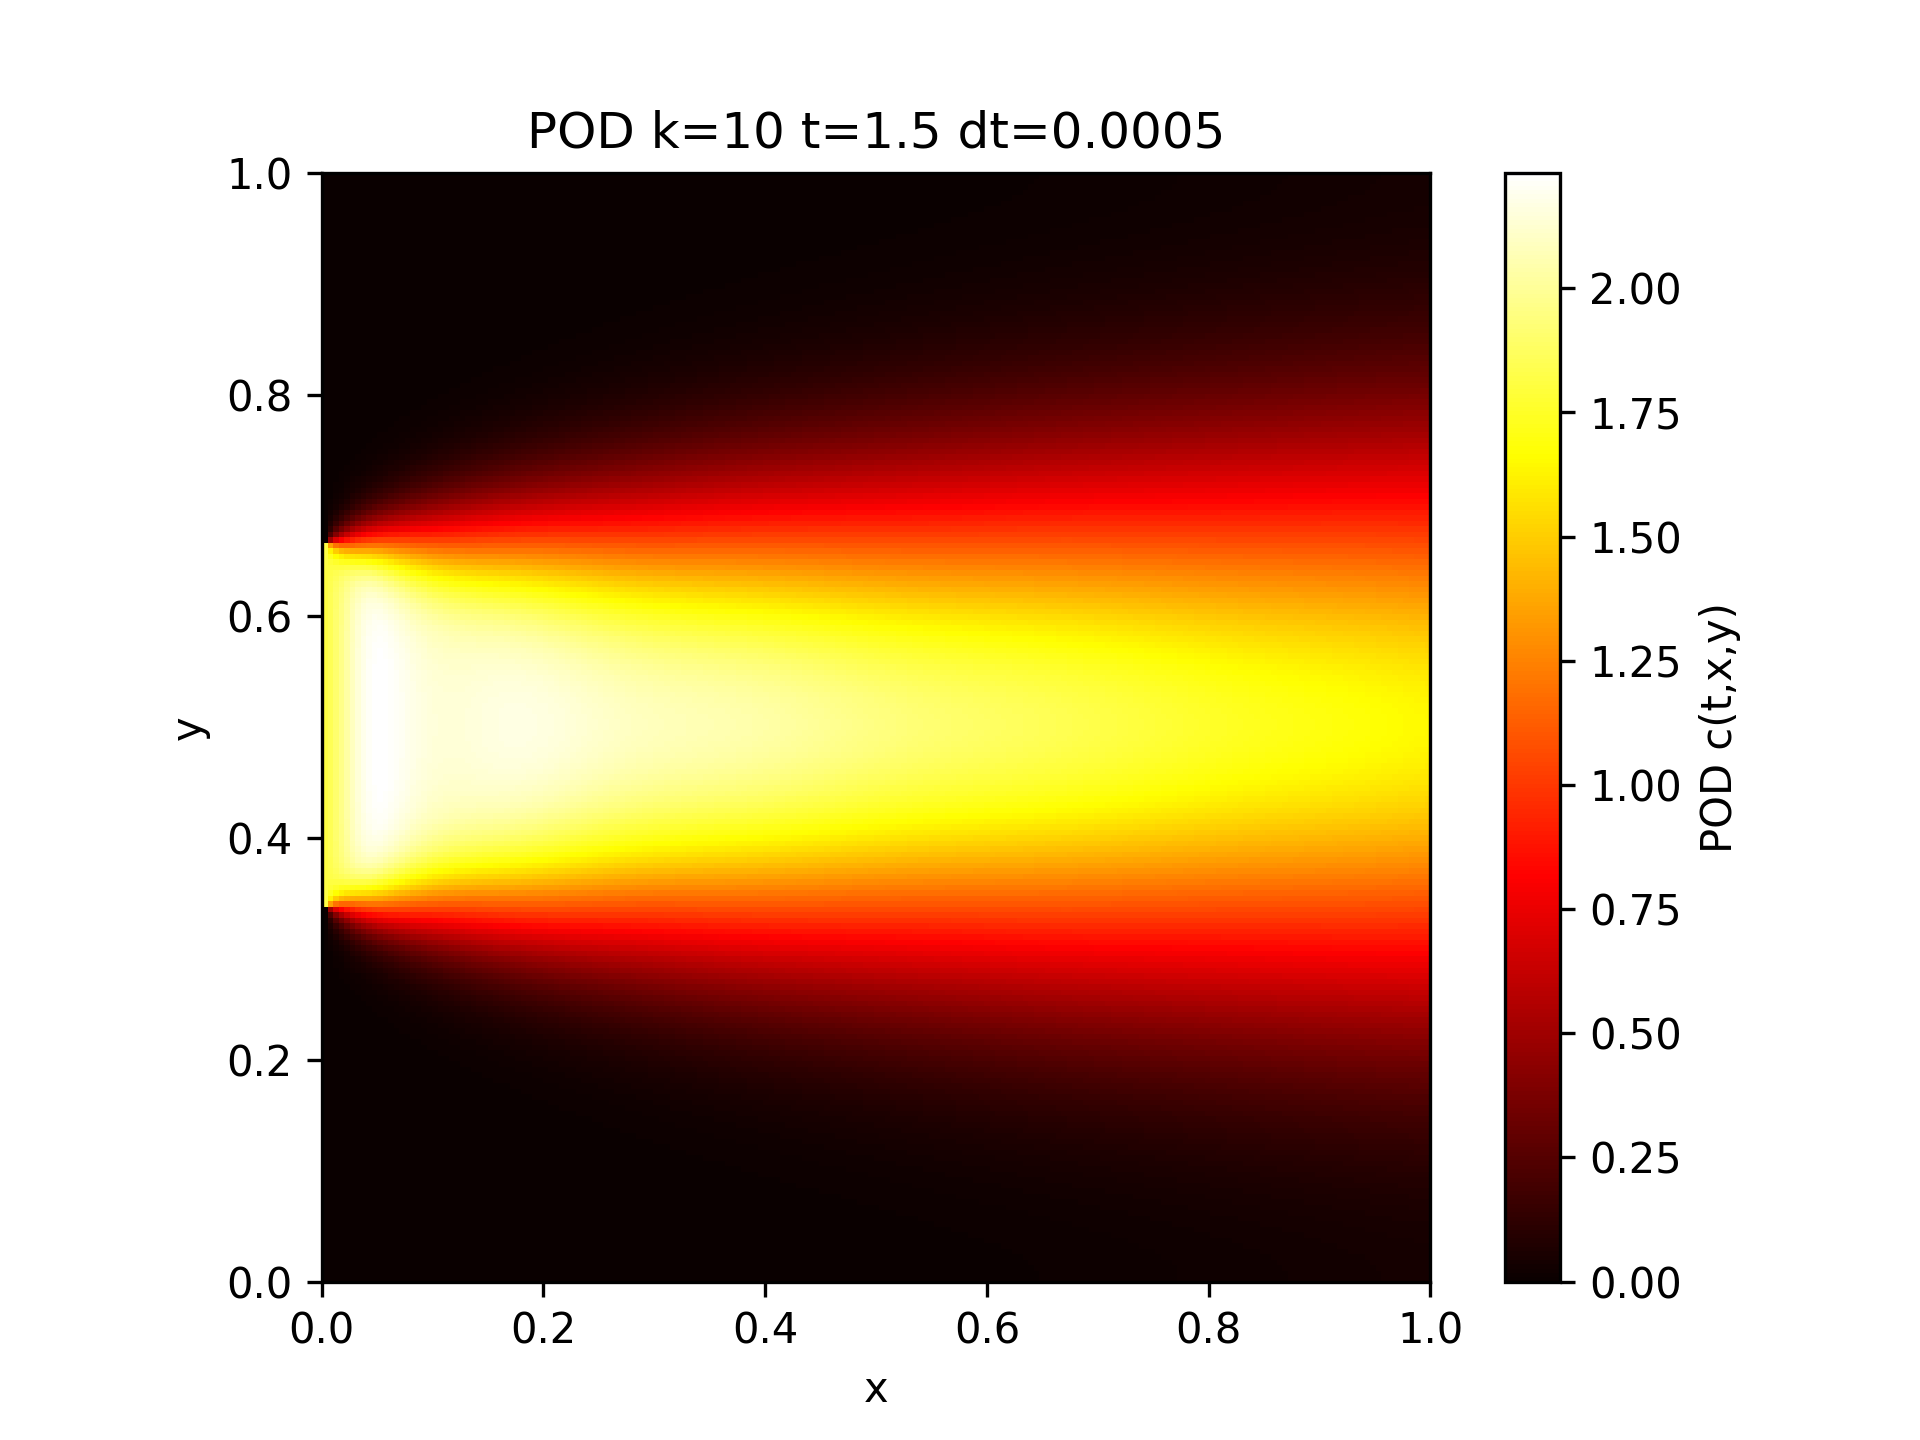
\includegraphics[width=\textwidth]{POD k=10 t=1.5 dt=0.0005.png}
        \caption{POD k=10 t=1.5 dt=0.0005}
        \label{POD k=10 t=1.5 dt=0.0005}
    \end{subfigure}
    
    \caption{results of POD k = 10}
    \label{results of POD k = 10}
\end{figure}

\begin{figure}[htbp]
    \centering
    % 2x2 排列
    \begin{subfigure}{0.45\textwidth}
        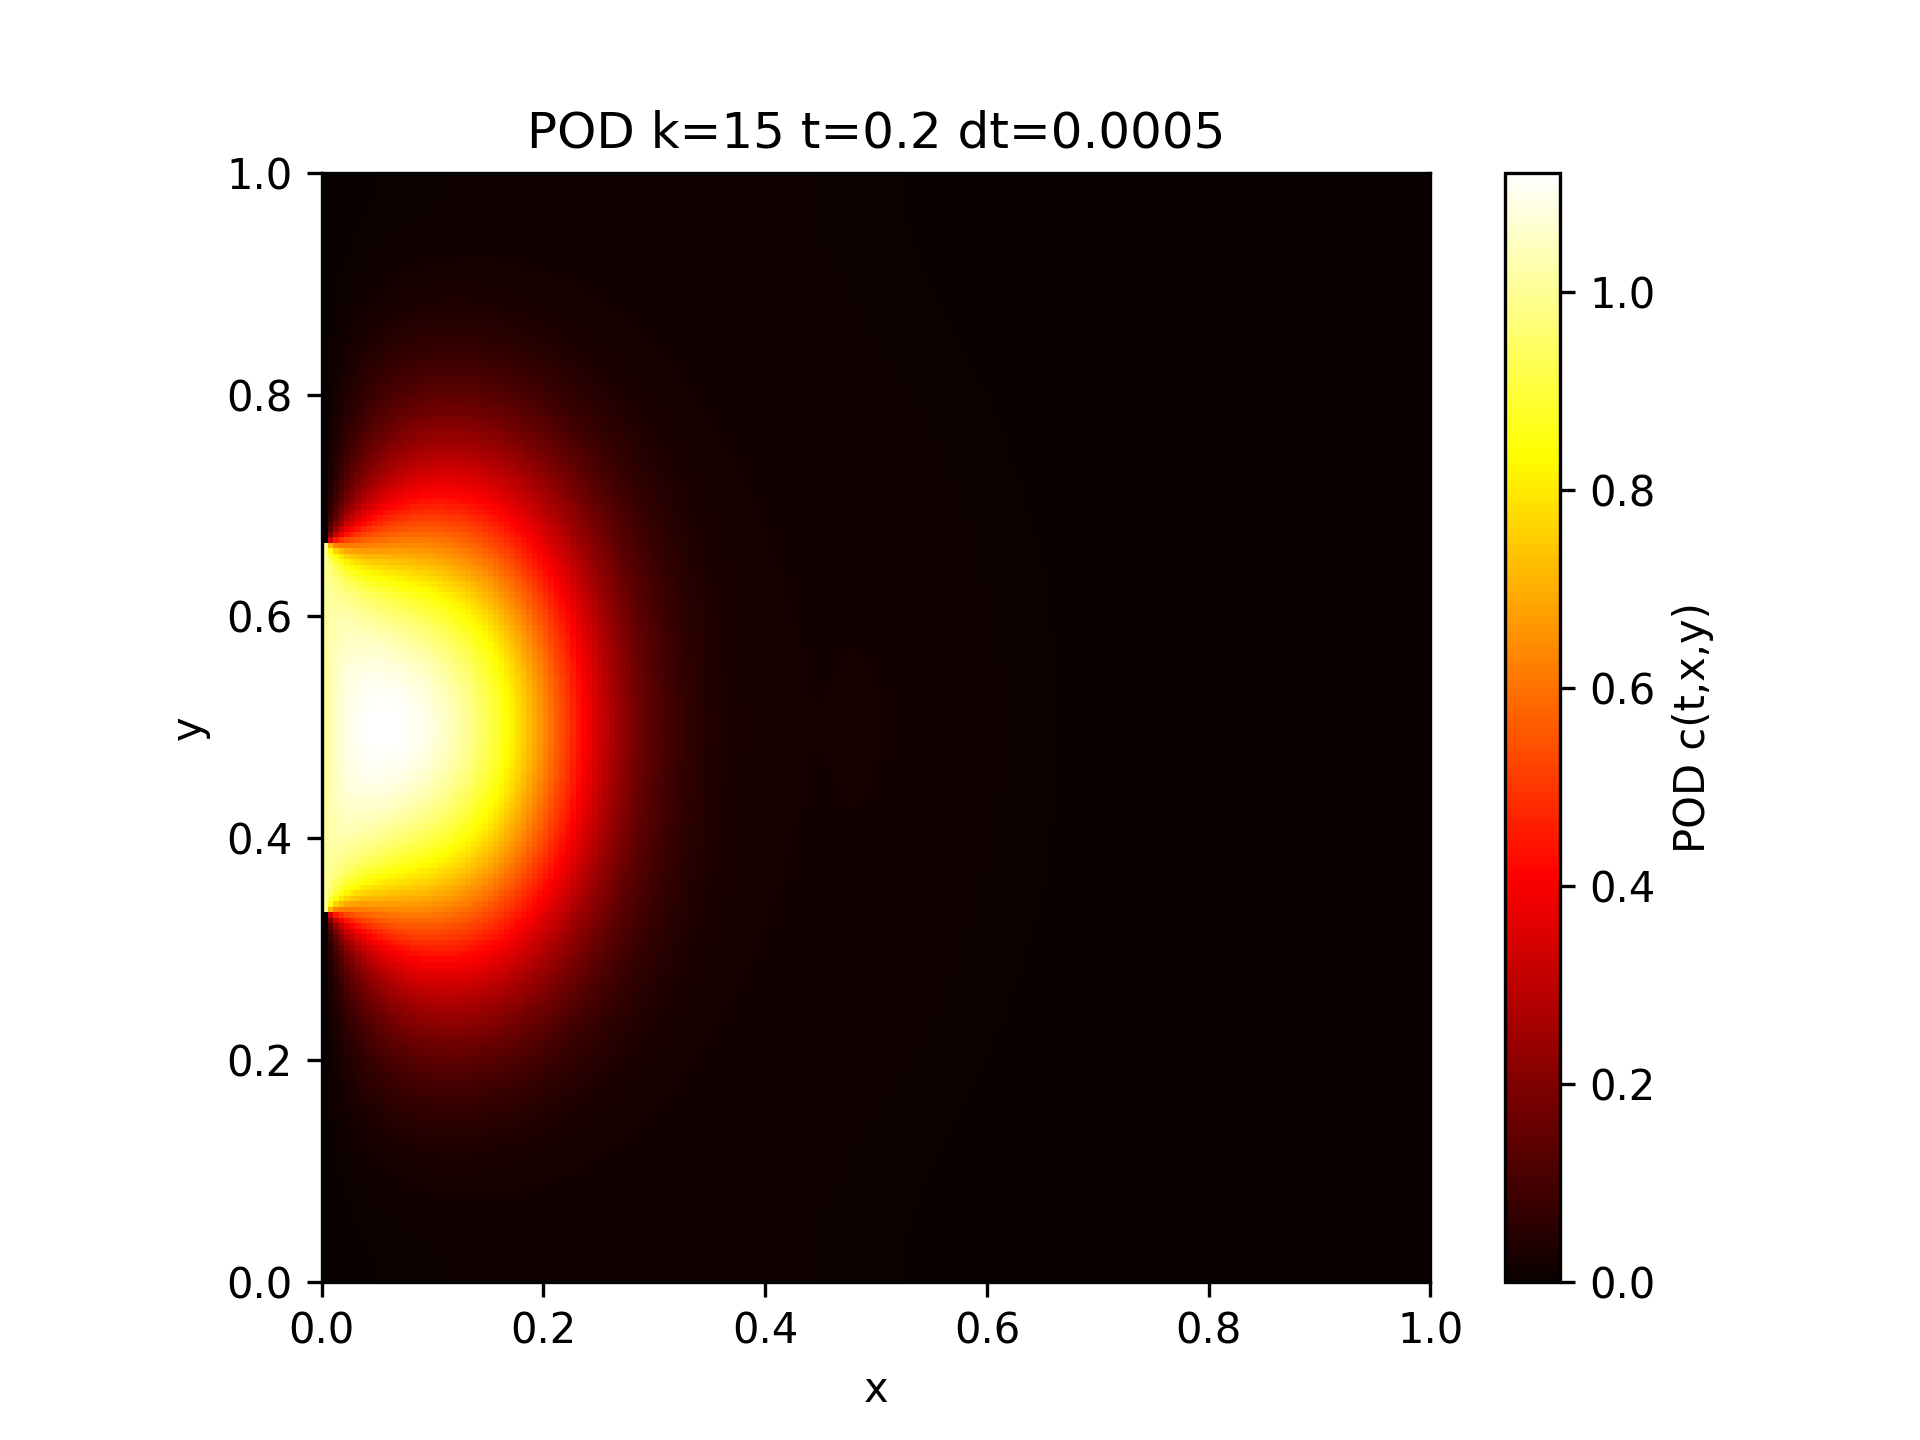
\includegraphics[width=\textwidth]{POD k=15 t=0.2 dt=0.0005.png}
        \caption{POD k=15 t=0.2 dt=0.0005}
        \label{POD k=15 t=0.2 dt=0.0005}
    \end{subfigure}
    \hfill
    \begin{subfigure}{0.45\textwidth}
        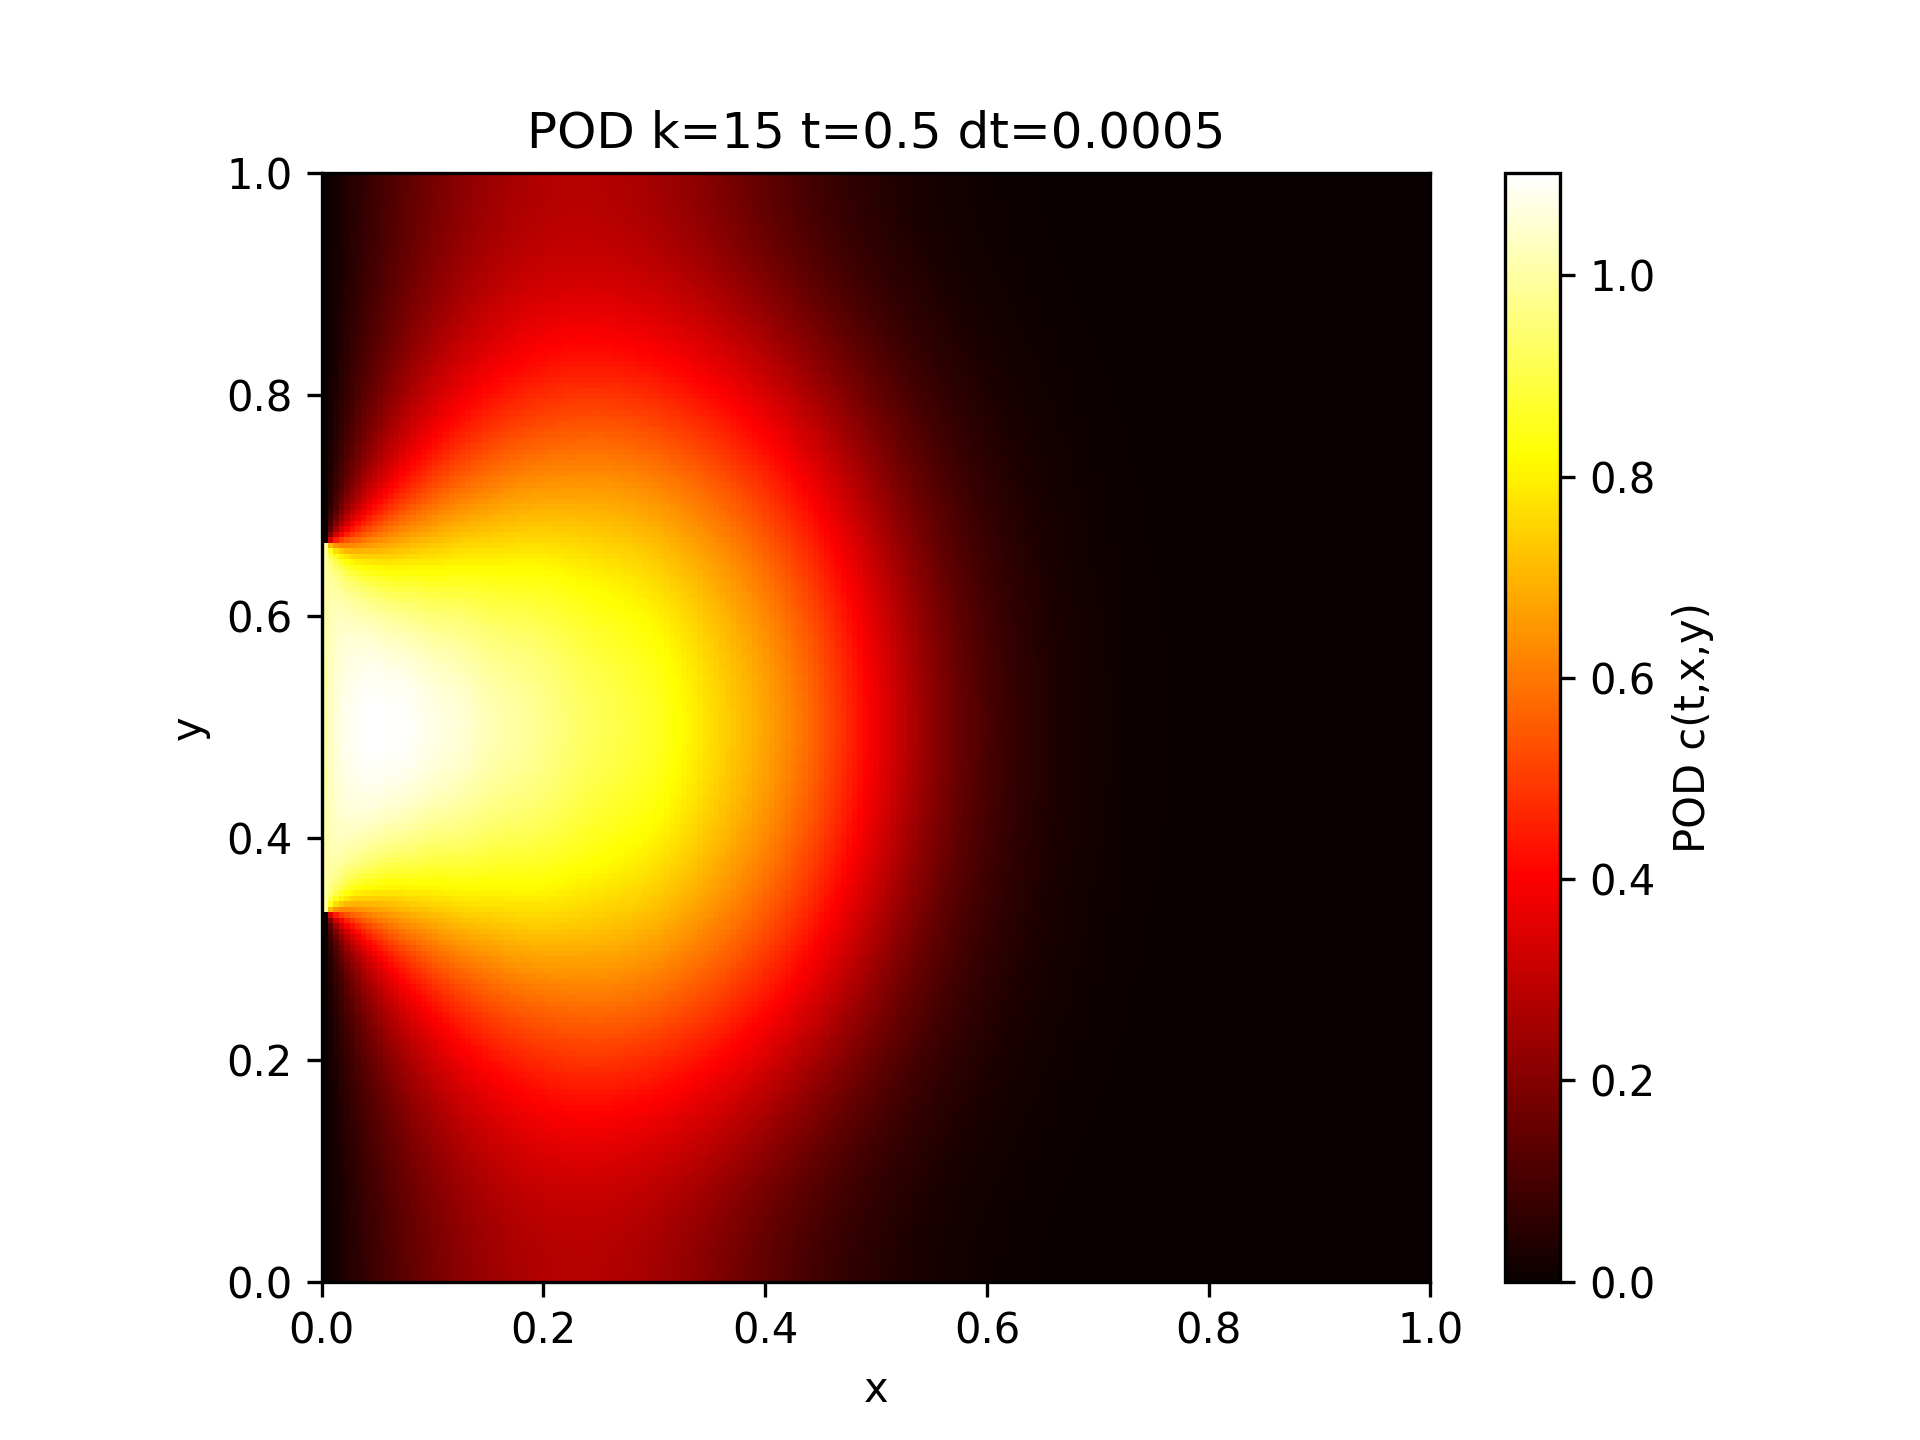
\includegraphics[width=\textwidth]{POD k=15 t=0.5 dt=0.0005.png}
        \caption{POD k=15 t=0.5 dt=0.0005}
        \label{POD k=15 t=0.5 dt=0.0005}
    \end{subfigure}
    
    \vspace{0.5cm}  % 垂直间距
    
    \begin{subfigure}{0.45\textwidth}
        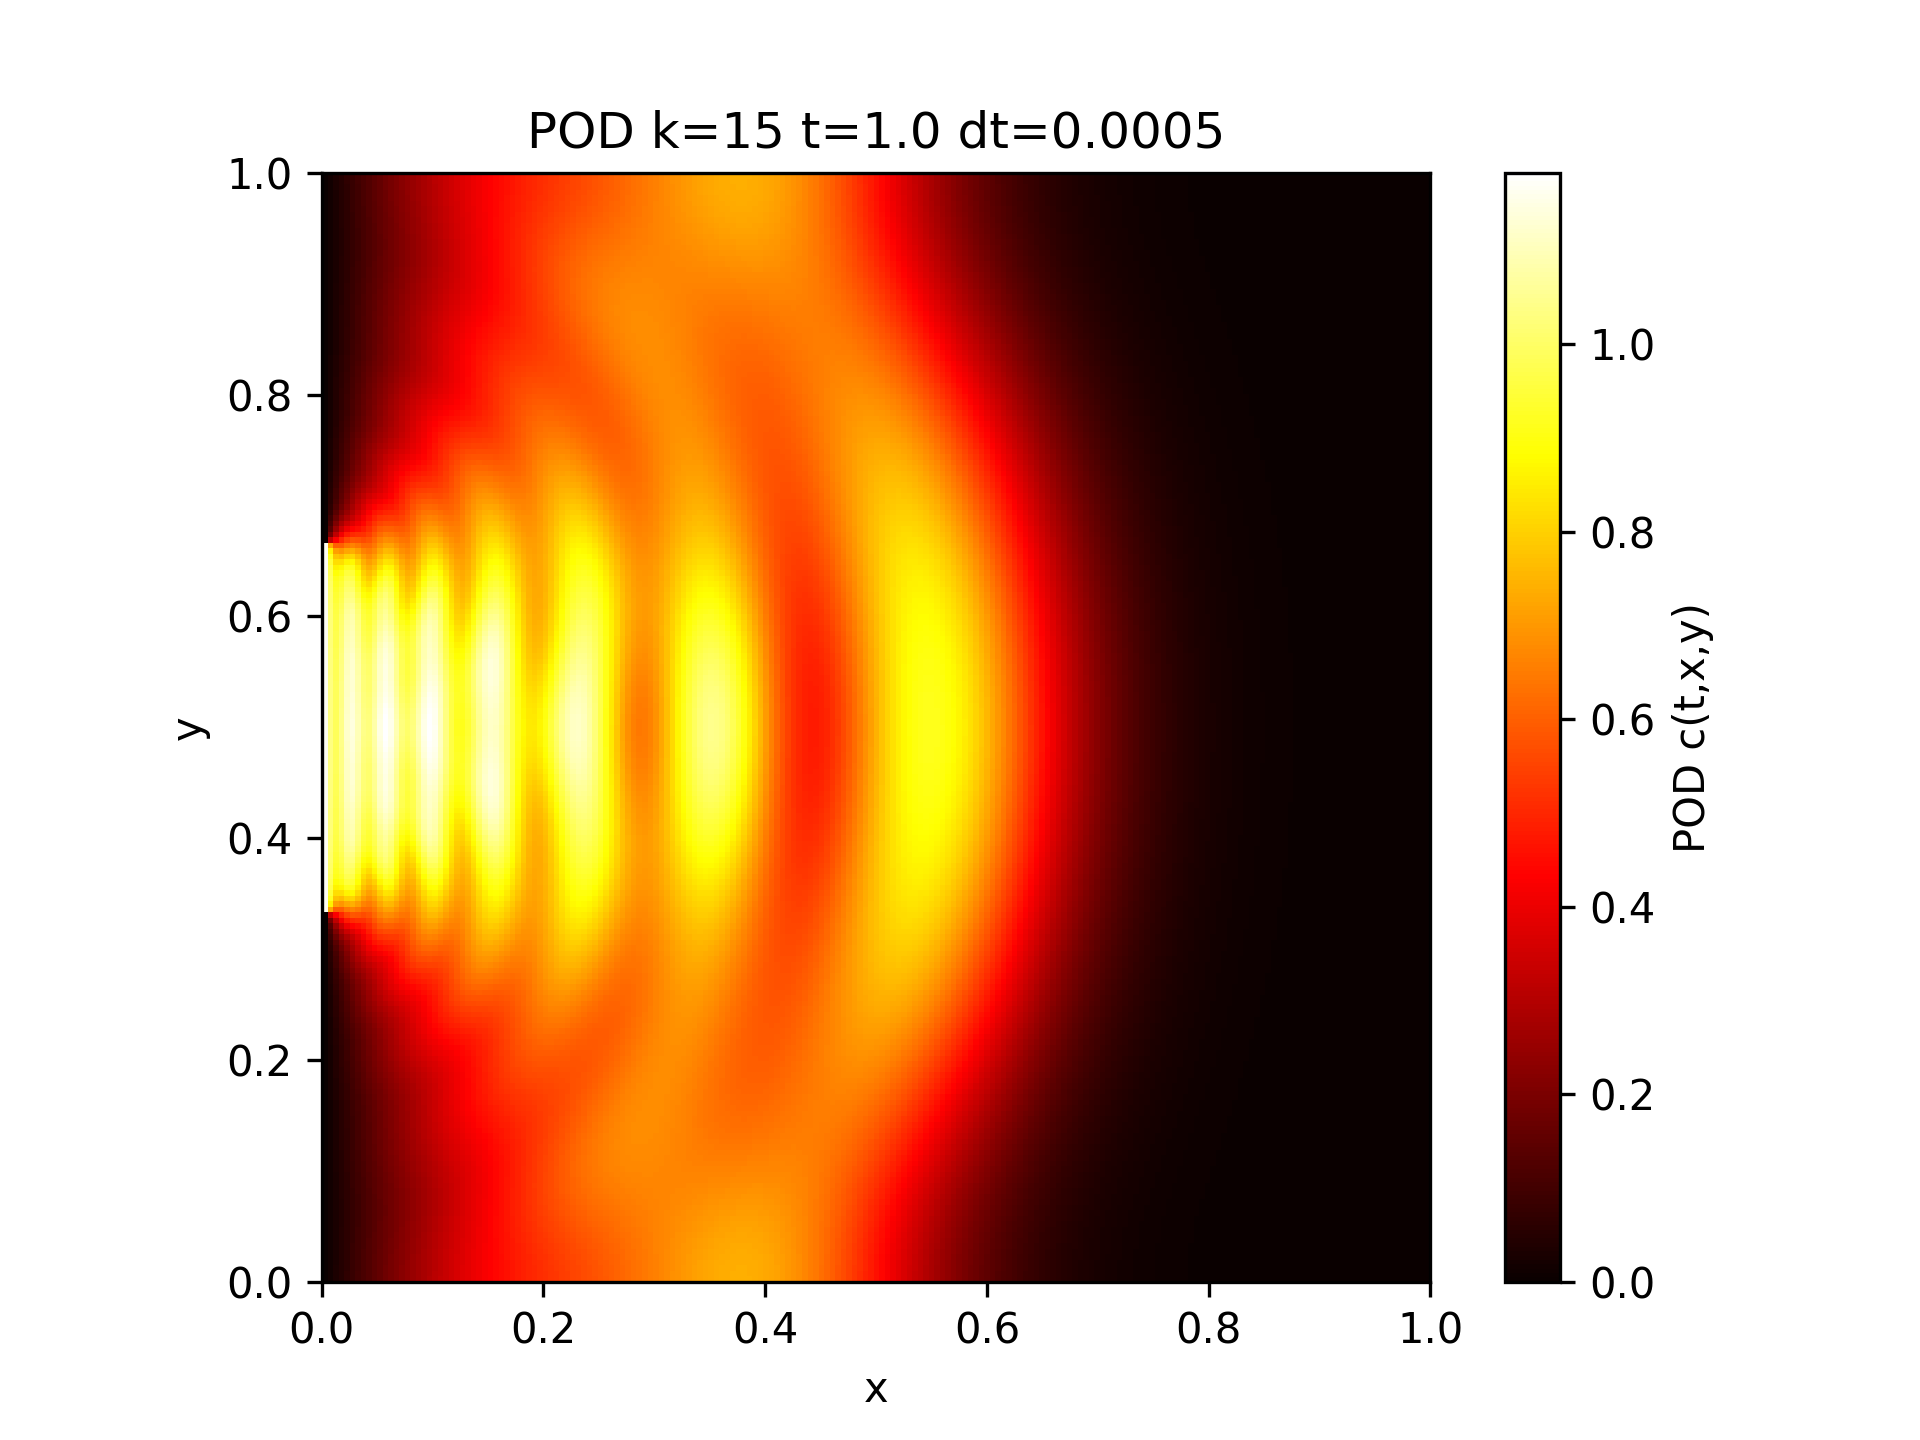
\includegraphics[width=\textwidth]{POD k=15 t=1.0 dt=0.0005.png}
        \caption{POD k=15 t=1.0 dt=0.0005}
        \label{POD k=15 t=1.0 dt=0.0005}
    \end{subfigure}
    \hfill
    \begin{subfigure}{0.45\textwidth}
        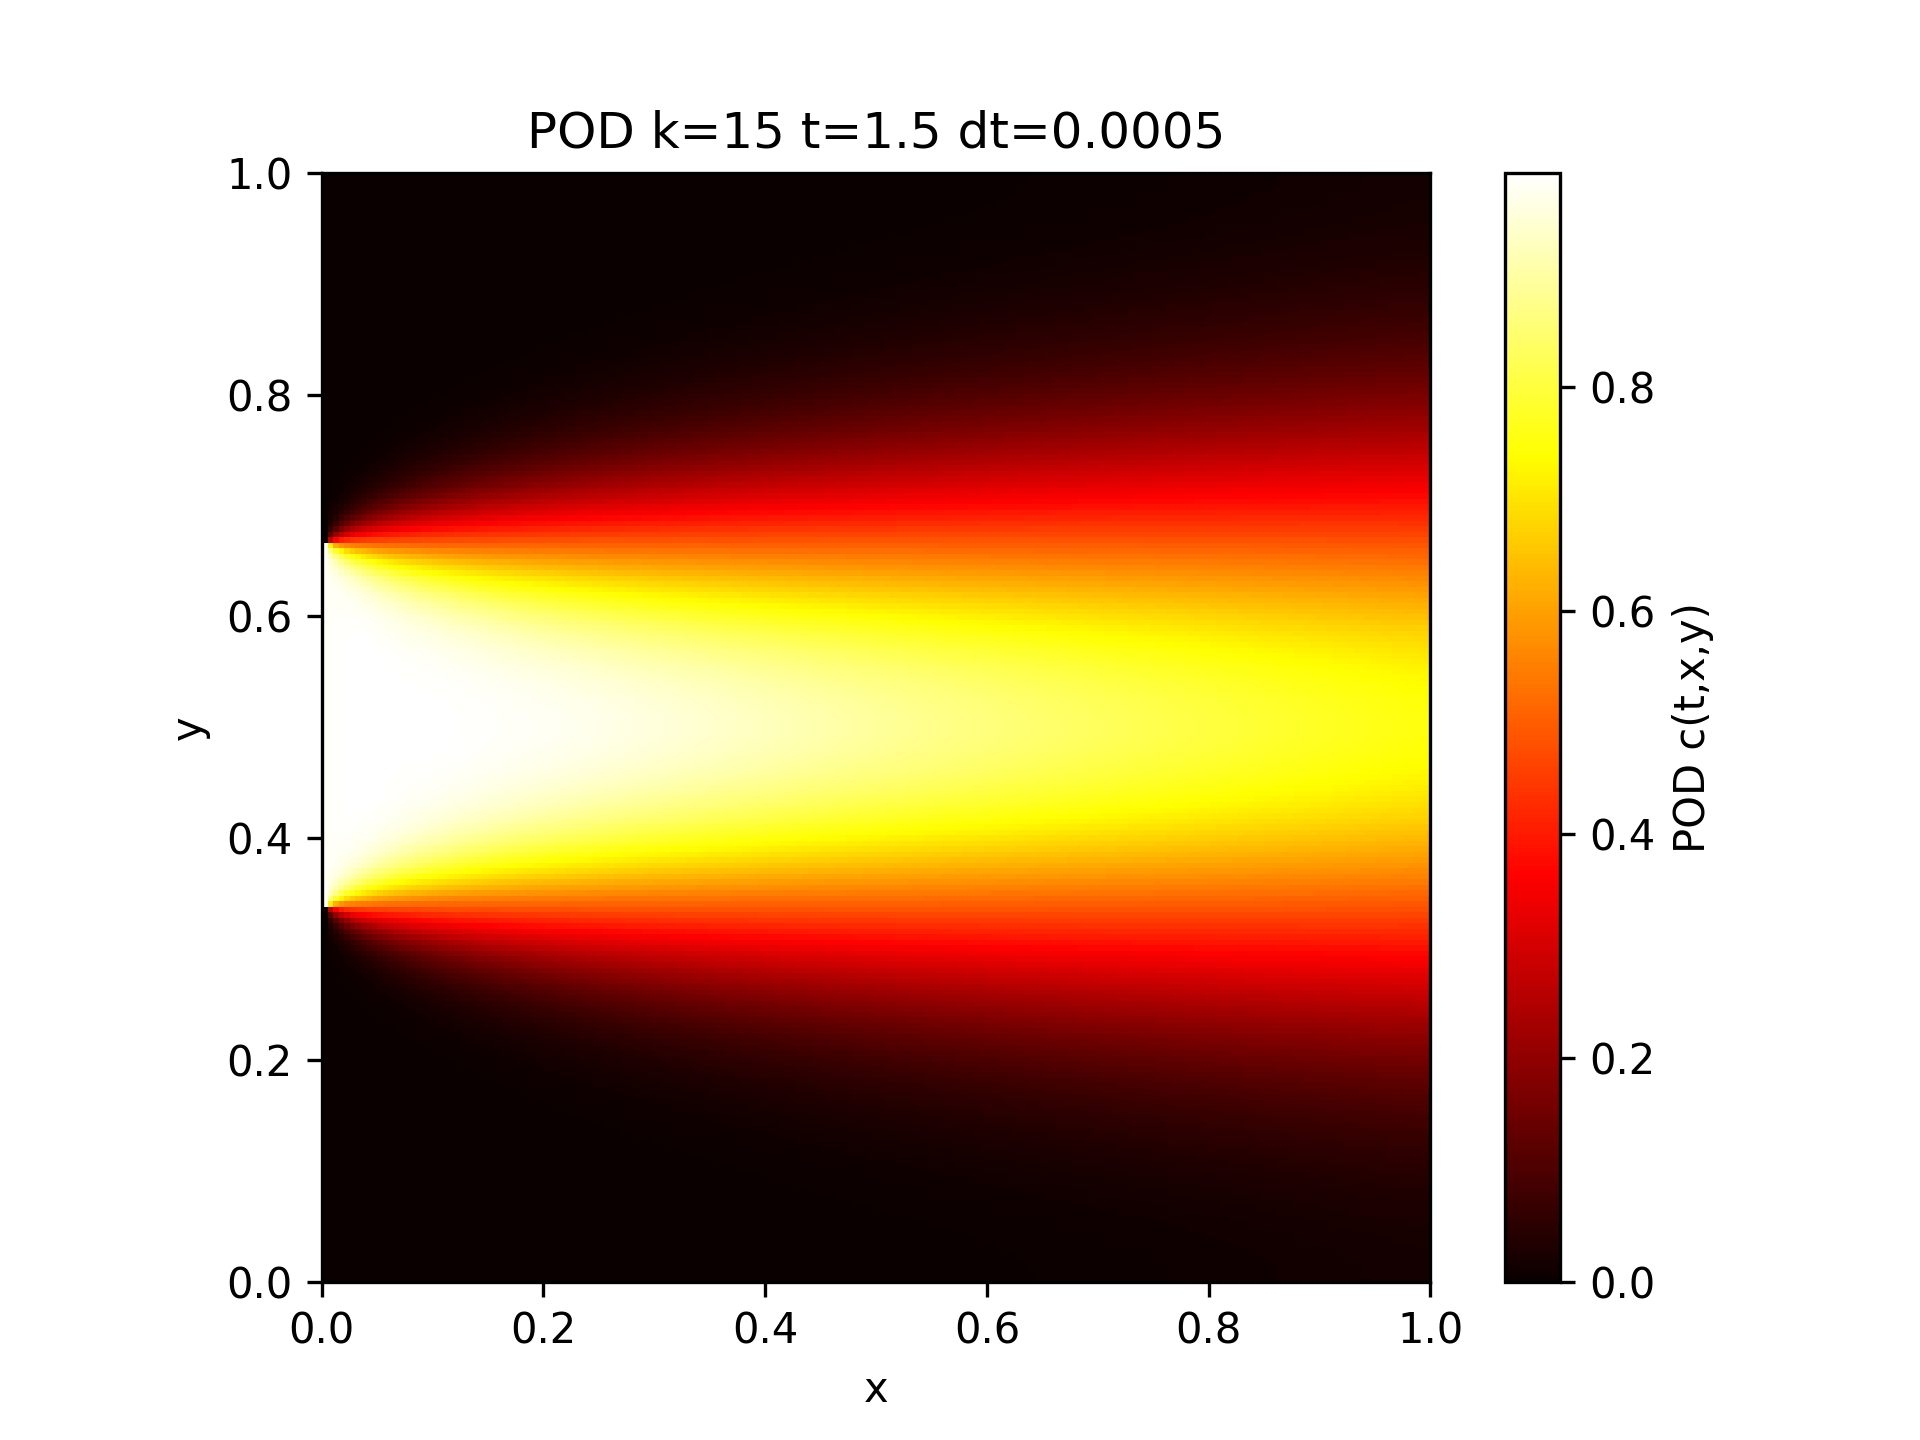
\includegraphics[width=\textwidth]{POD k=15 t=1.5 dt=0.0005.png}
        \caption{POD k=15 t=1.5 dt=0.0005}
        \label{POD k=15 t=1.5 dt=0.0005}
    \end{subfigure}
    
    \caption{results of POD k = 15}
    \label{results of POD k = 15}
\end{figure}
\section{问题3}
采用动力学模态分解方法进行计算.
\subsection{计算方法}
由问题2启发,做动力学建模$\mathbf{c}(t+\Delta t) = K\mathbf{c}(t)+b$,即线性模型,进而有\begin{equation}
    \begin{pmatrix}
        \mathbf{c}(t+\Delta t)\\1
    \end{pmatrix}
    =
    \begin{pmatrix}
        K & b\\0 & 1
    \end{pmatrix}
    \begin{pmatrix}
        \mathbf{c}(t)\\1
    \end{pmatrix}
\end{equation}
记对应动力学矩阵为$\bar{K}$。依然设定$N_{snap}=100$,对$[0,T]$做等距划分,得到数据集,每个向量末尾分别添加元素1,共101个向量。
取$\bar{X}$为前100个向量,$\bar{Y}$为后100个向量,以近似$\bar{Y}=\bar{K}\bar{X}$。
\par 对$\bar{X}$做SVD,设秩为$r$,对SVD做满秩截断,Koopman矩阵应为$\bar{K}=YV\Sigma^{-1}U^*$,我们转而去求$\tilde{K}=U^{*}YV\Sigma^{-1}$的特征对
$(\tilde{\lambda_j},\tilde{w_j},\tilde{v_j})_{j=0}^{r-1}$,
进而可以得到$\bar{K}$的特征对$(\lambda_j,w_j,v_j)_{j=0}^{r-1}$,满足转换关系\begin{equation}
    \begin{cases}
        \lambda_j=\tilde{\lambda_j}\\
        w_j=U\tilde{w_j}\\
        v_j=YV\Sigma^{-1}\tilde{v_j}
    \end{cases}
\end{equation}
将$W,V$做双正交归一化,即可以认为$W^*V=I$。最后以Koopman模式计算$\mathbf{c}(m)$。
\subsection{Koopman算子的谱与Koopman模式}
所得到的Koopman算子的谱如图\ref{DMD Eigenvalues}所示。\begin{figure}[htbp]
    \centering
    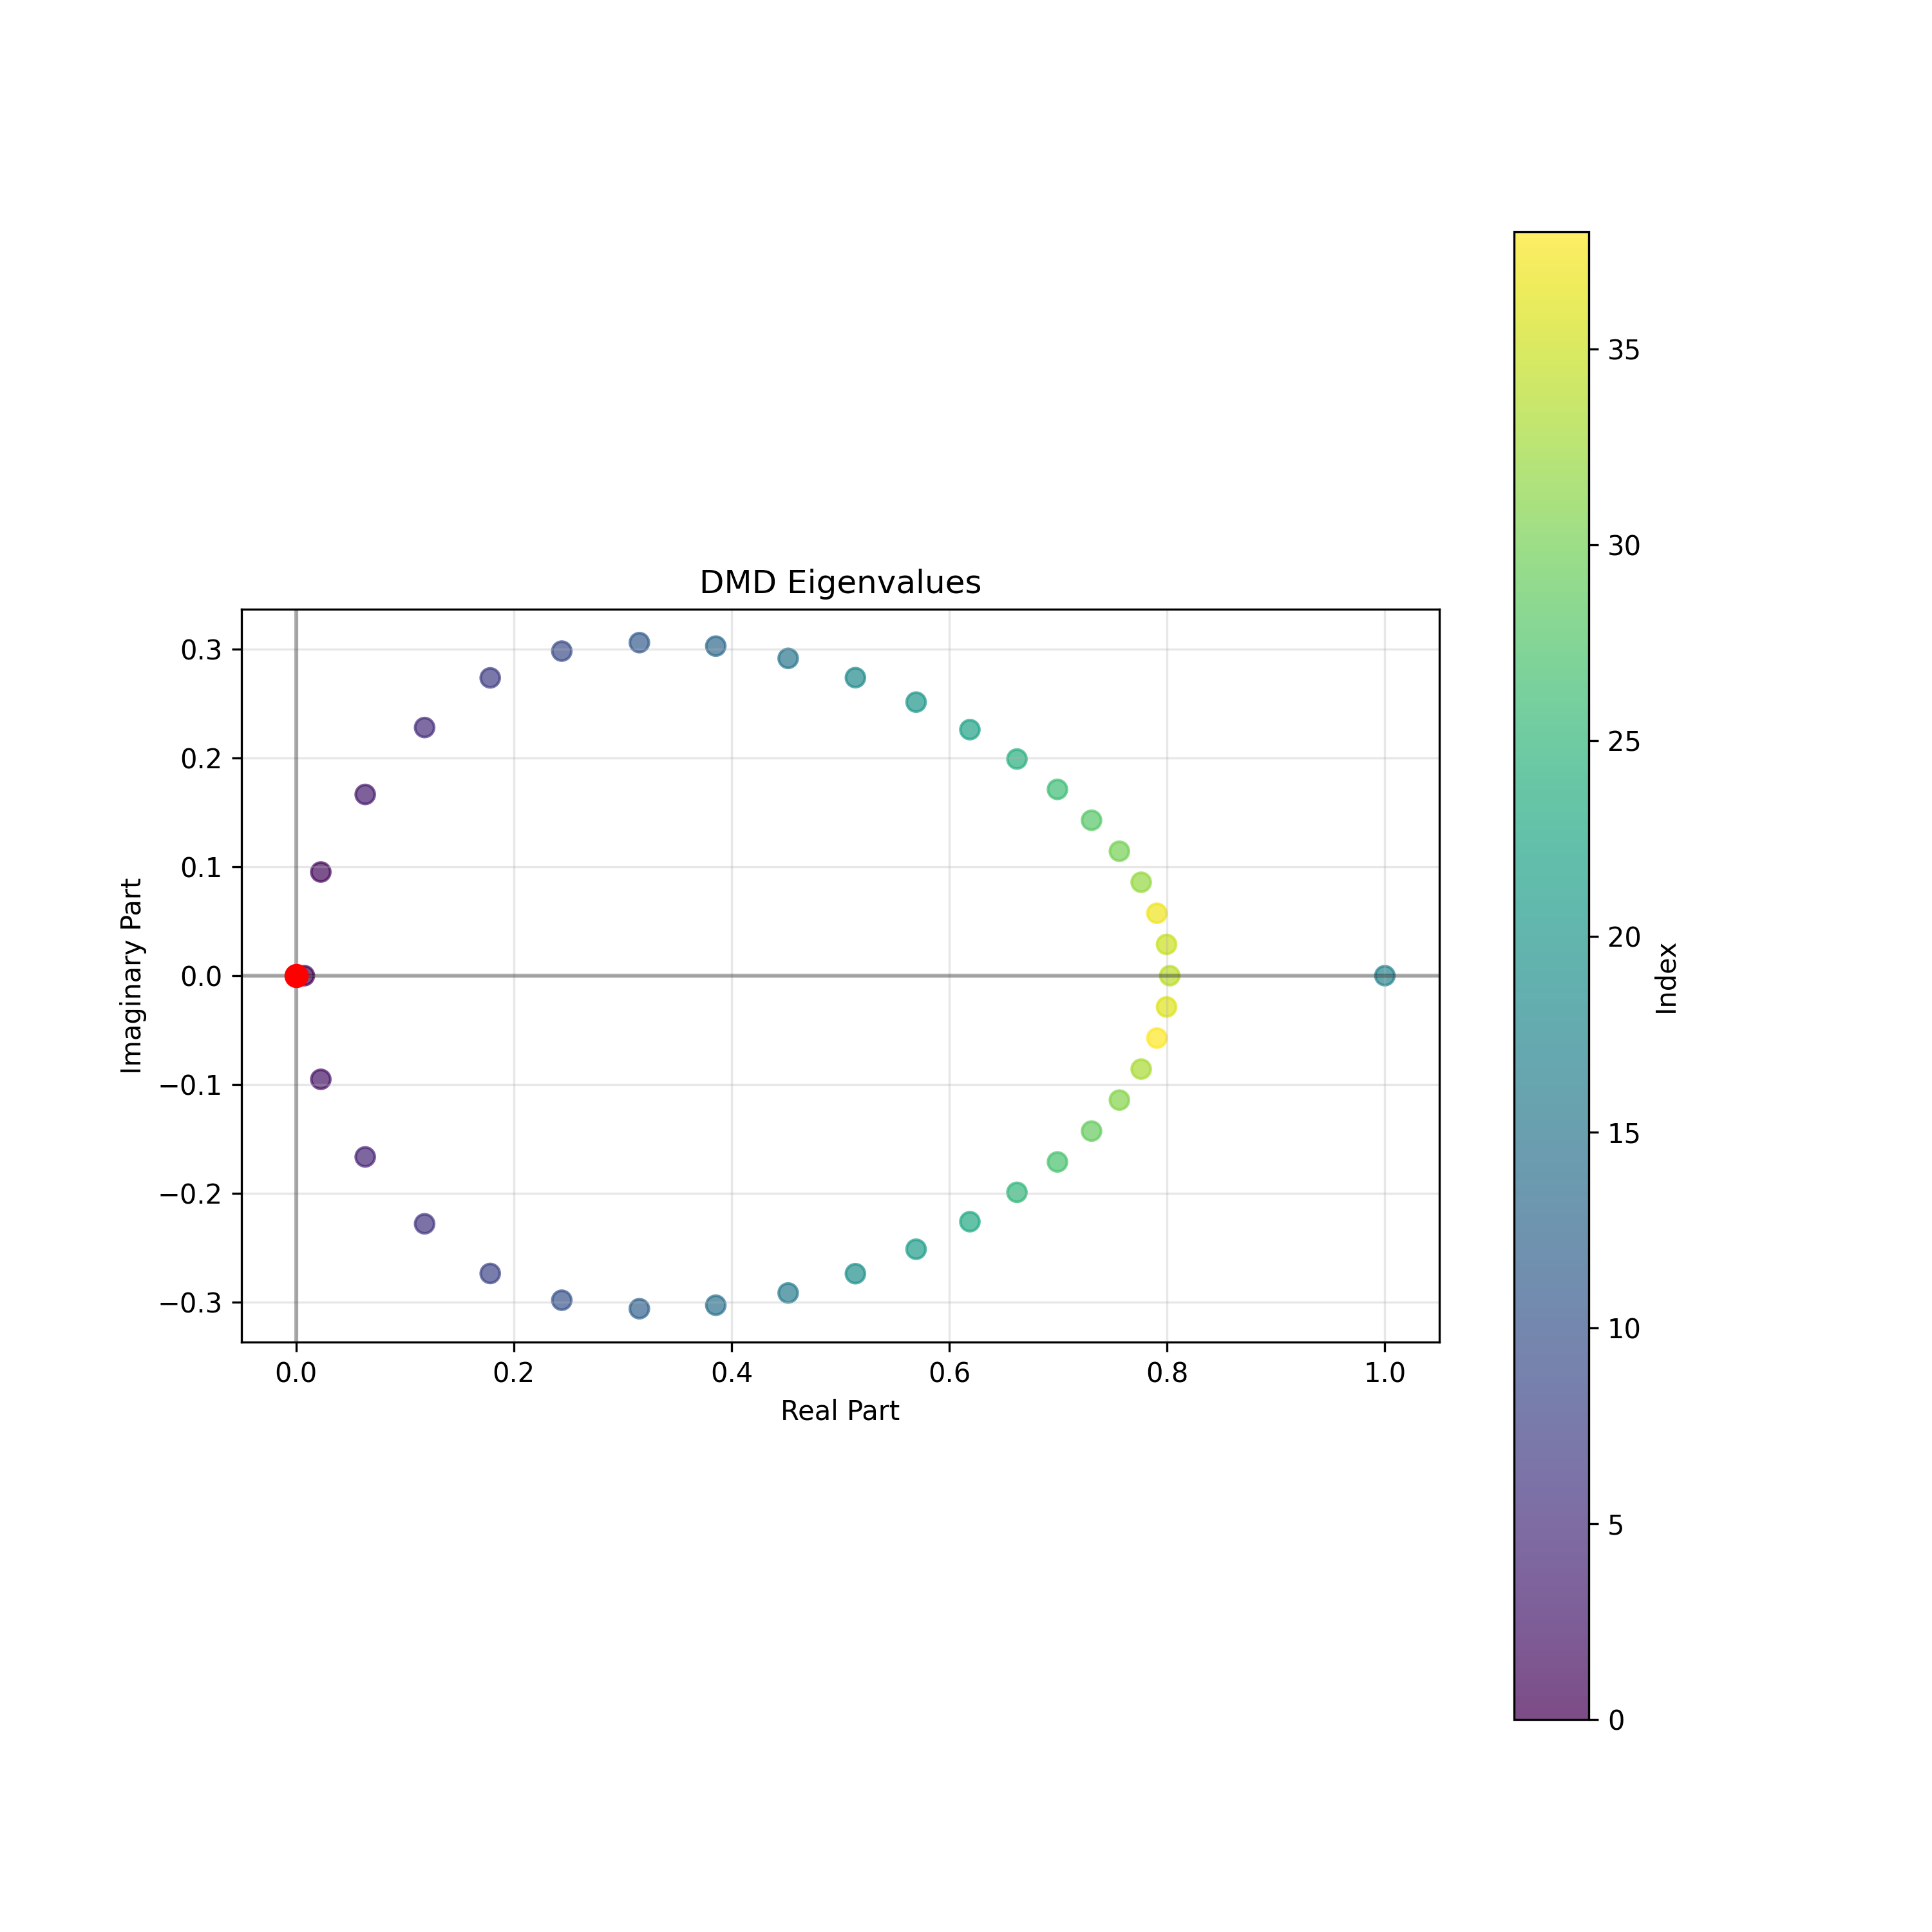
\includegraphics[width=\textwidth]{DMD Eigenvalues.png}
        \caption{DMD Eigenvalues}
        \label{DMD Eigenvalues}
\end{figure}
对应Koopman模式:\begin{equation}
    \begin{cases}
        \bar{\mathbf{c}} = \begin{pmatrix}
            \mathbf{c} \\ 1
        \end{pmatrix}
        \\
        \bar{\mathbf{c}}(m) = \sum_{j=0}^{r-1}\lambda_j^m v_j w_j^* \bar{\mathbf{c}}(0)
    \end{cases}
\end{equation}
\subsection{结果展示}
计算结果展示如图\ref{results of DMD dt = 0.015}所示.
\begin{figure}[htbp]
    \centering
    % 2x2 排列
    \begin{subfigure}{0.45\textwidth}
        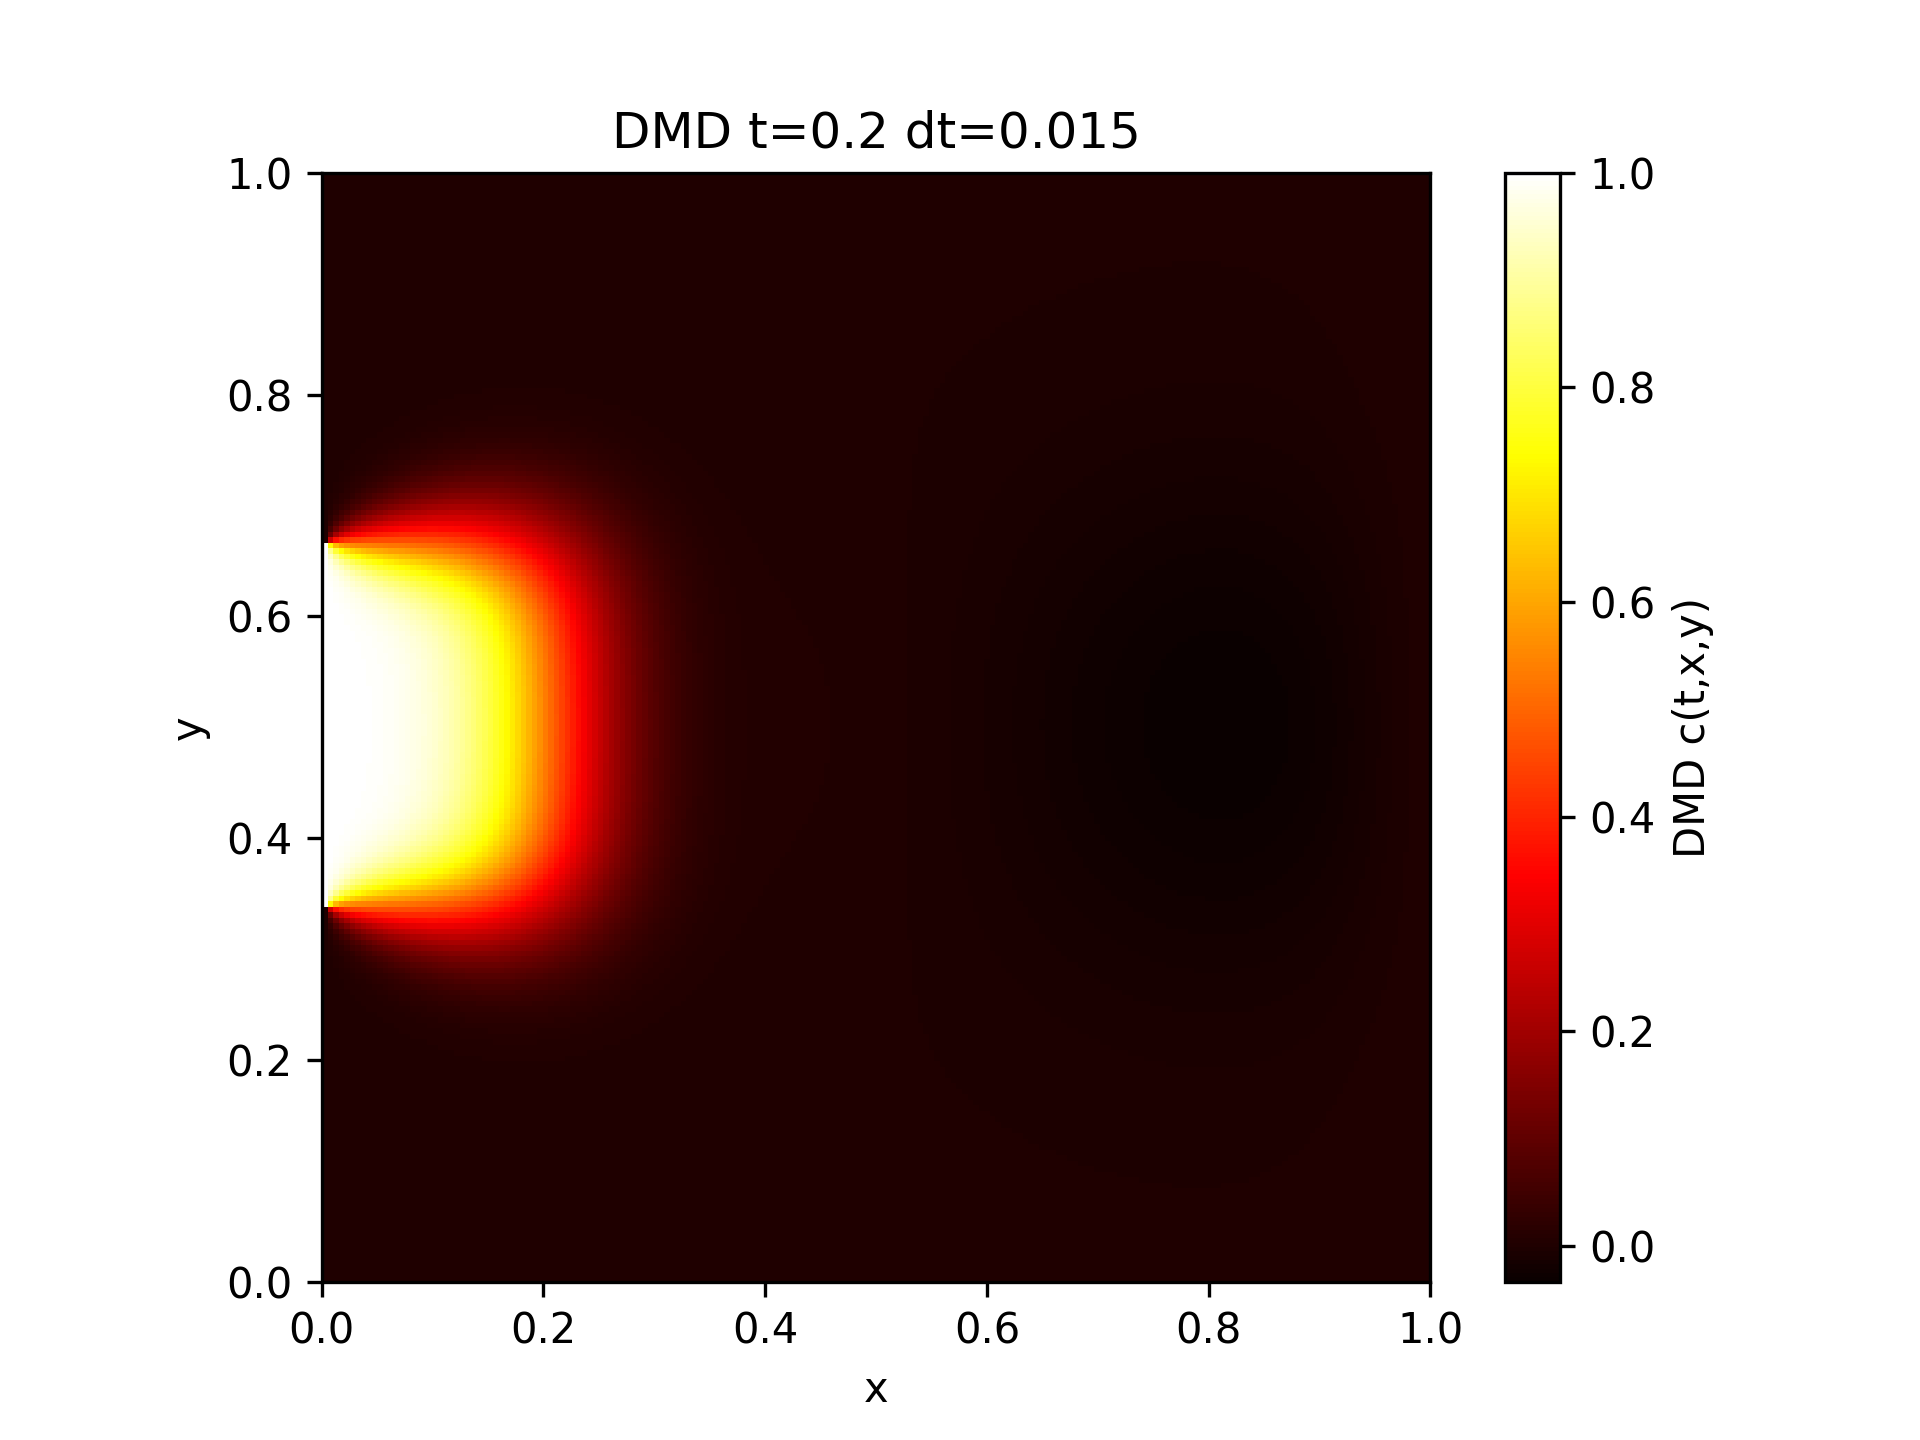
\includegraphics[width=\textwidth]{DMD t=0.2 dt=0.015.png}
        \caption{DMD t=0.2 dt=0.015}
        \label{DMD t=0.2 dt=0.015}
    \end{subfigure}
    \hfill
    \begin{subfigure}{0.45\textwidth}
        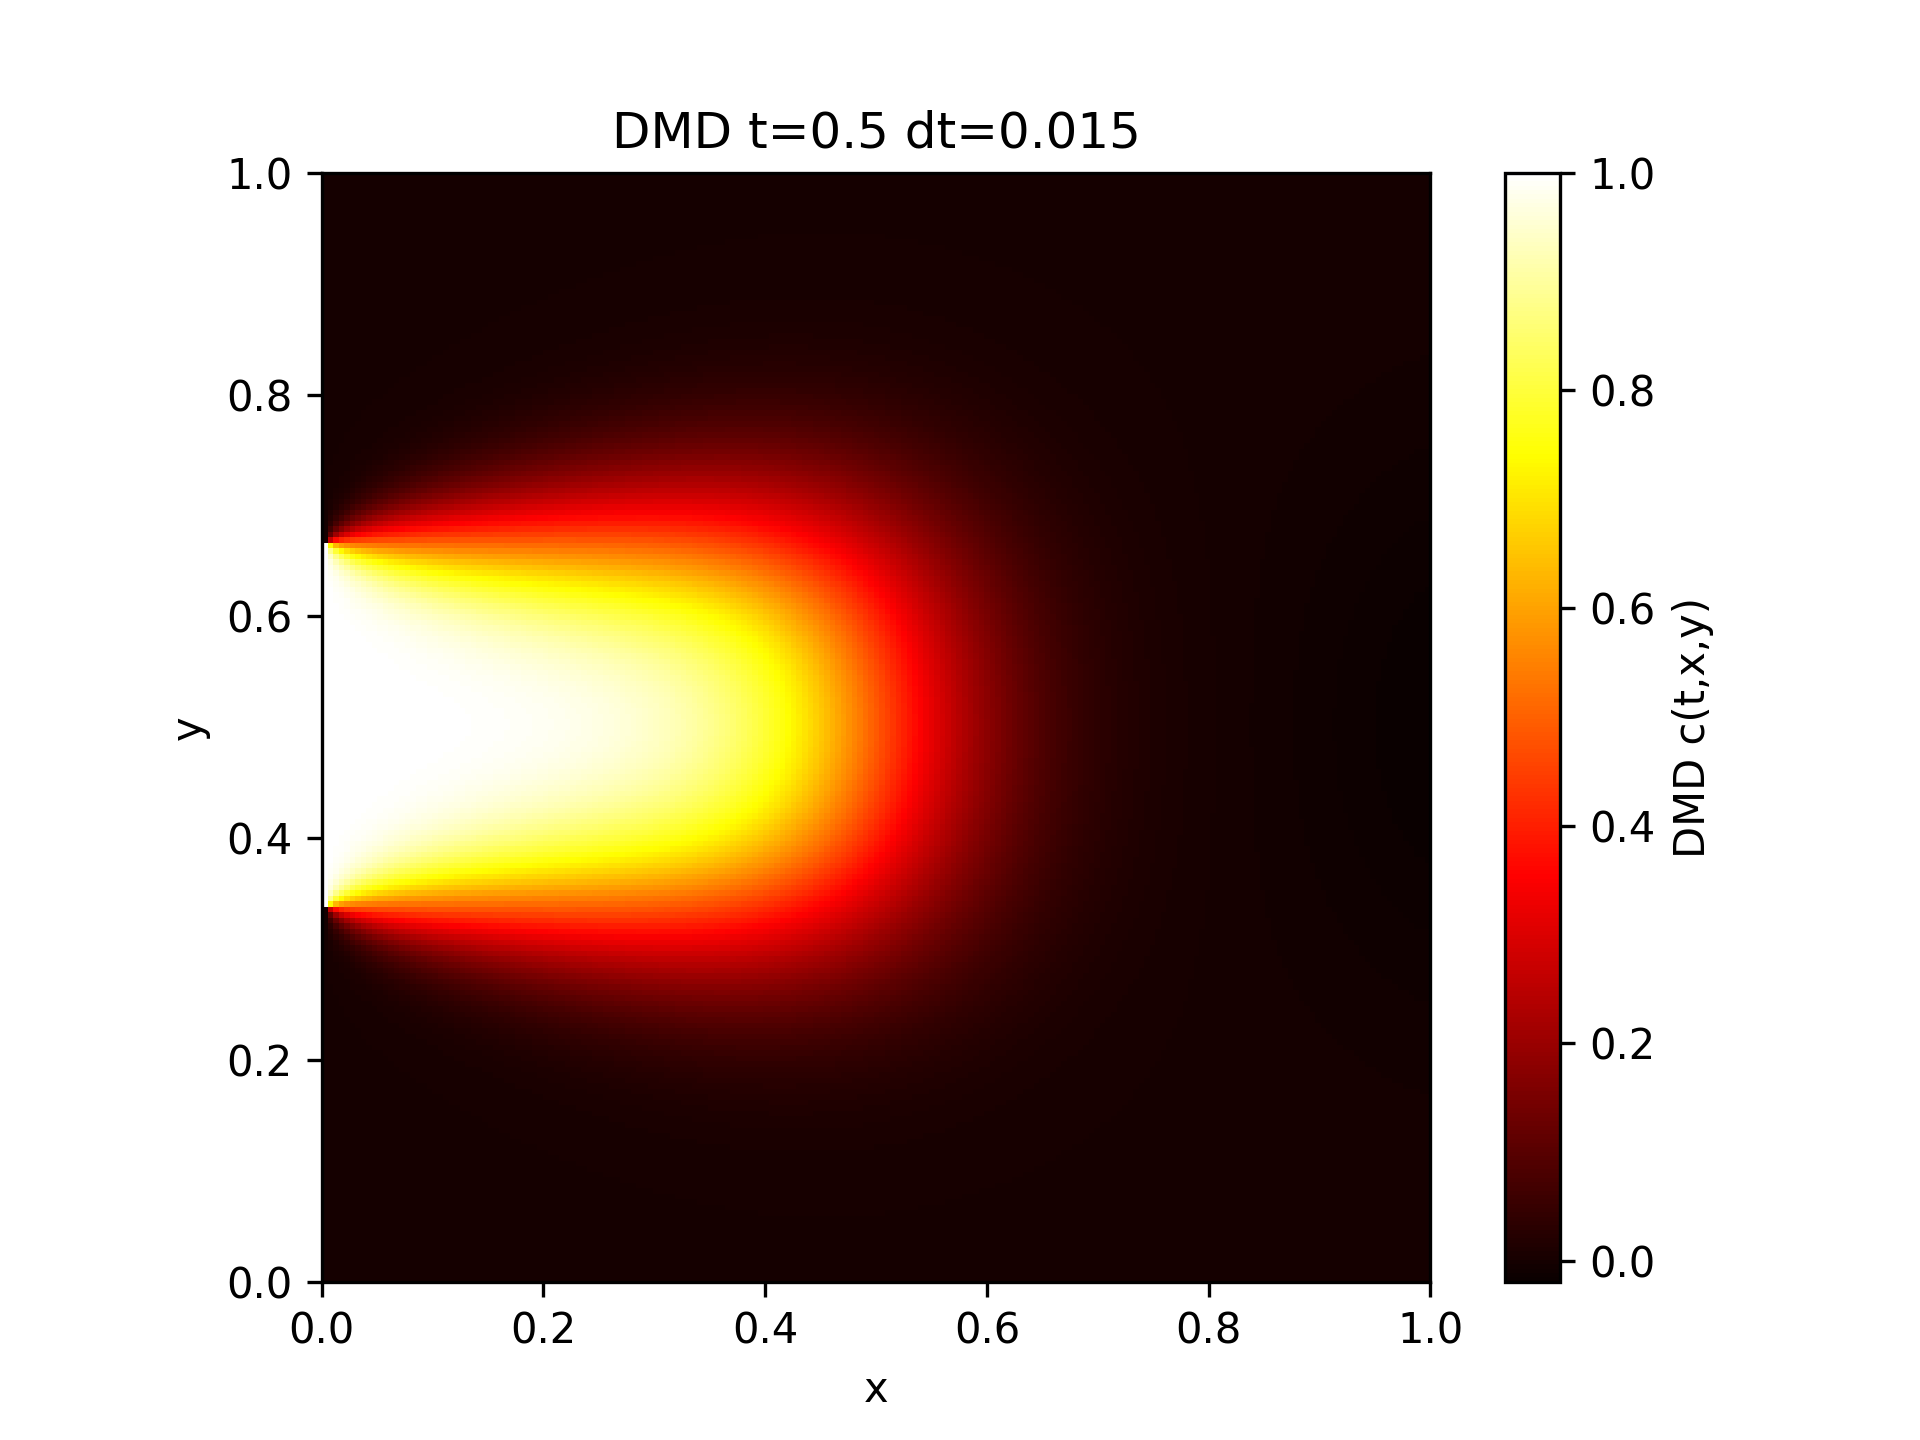
\includegraphics[width=\textwidth]{DMD t=0.5 dt=0.015.png}
        \caption{DMD t=0.5 dt=0.015}
        \label{DMD t=0.5 dt=0.015}
    \end{subfigure}
    
    \vspace{0.5cm}  % 垂直间距
    
    \begin{subfigure}{0.45\textwidth}
        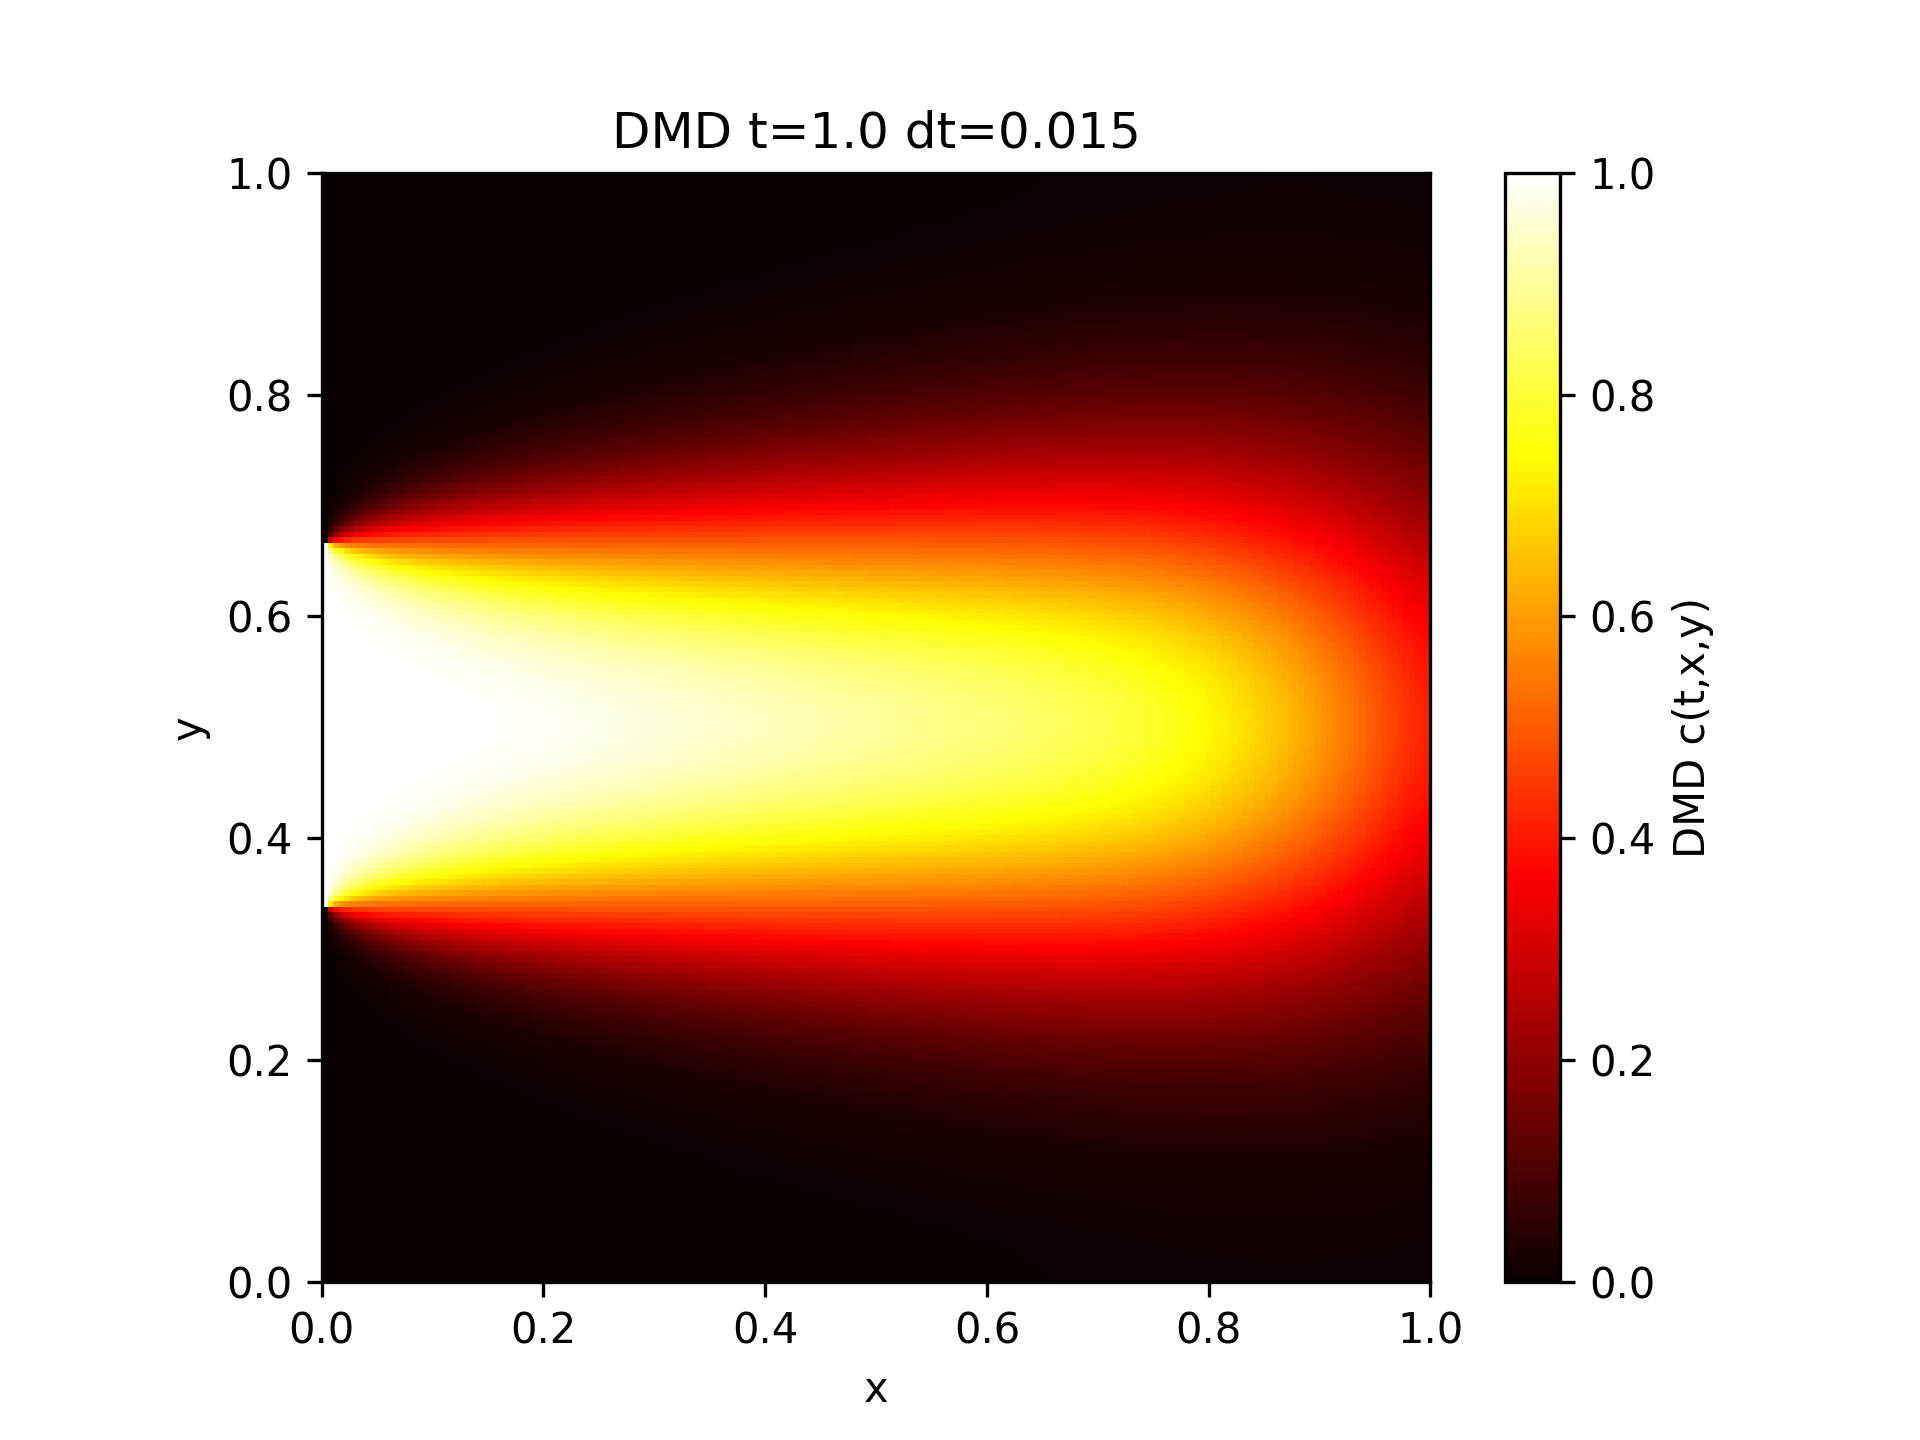
\includegraphics[width=\textwidth]{DMD t=1.0 dt=0.015.png}
        \caption{DMD t=1.0 dt=0.015}
        \label{FDMD t=1.0 dt=0.015}
    \end{subfigure}
    \hfill
    \begin{subfigure}{0.45\textwidth}
        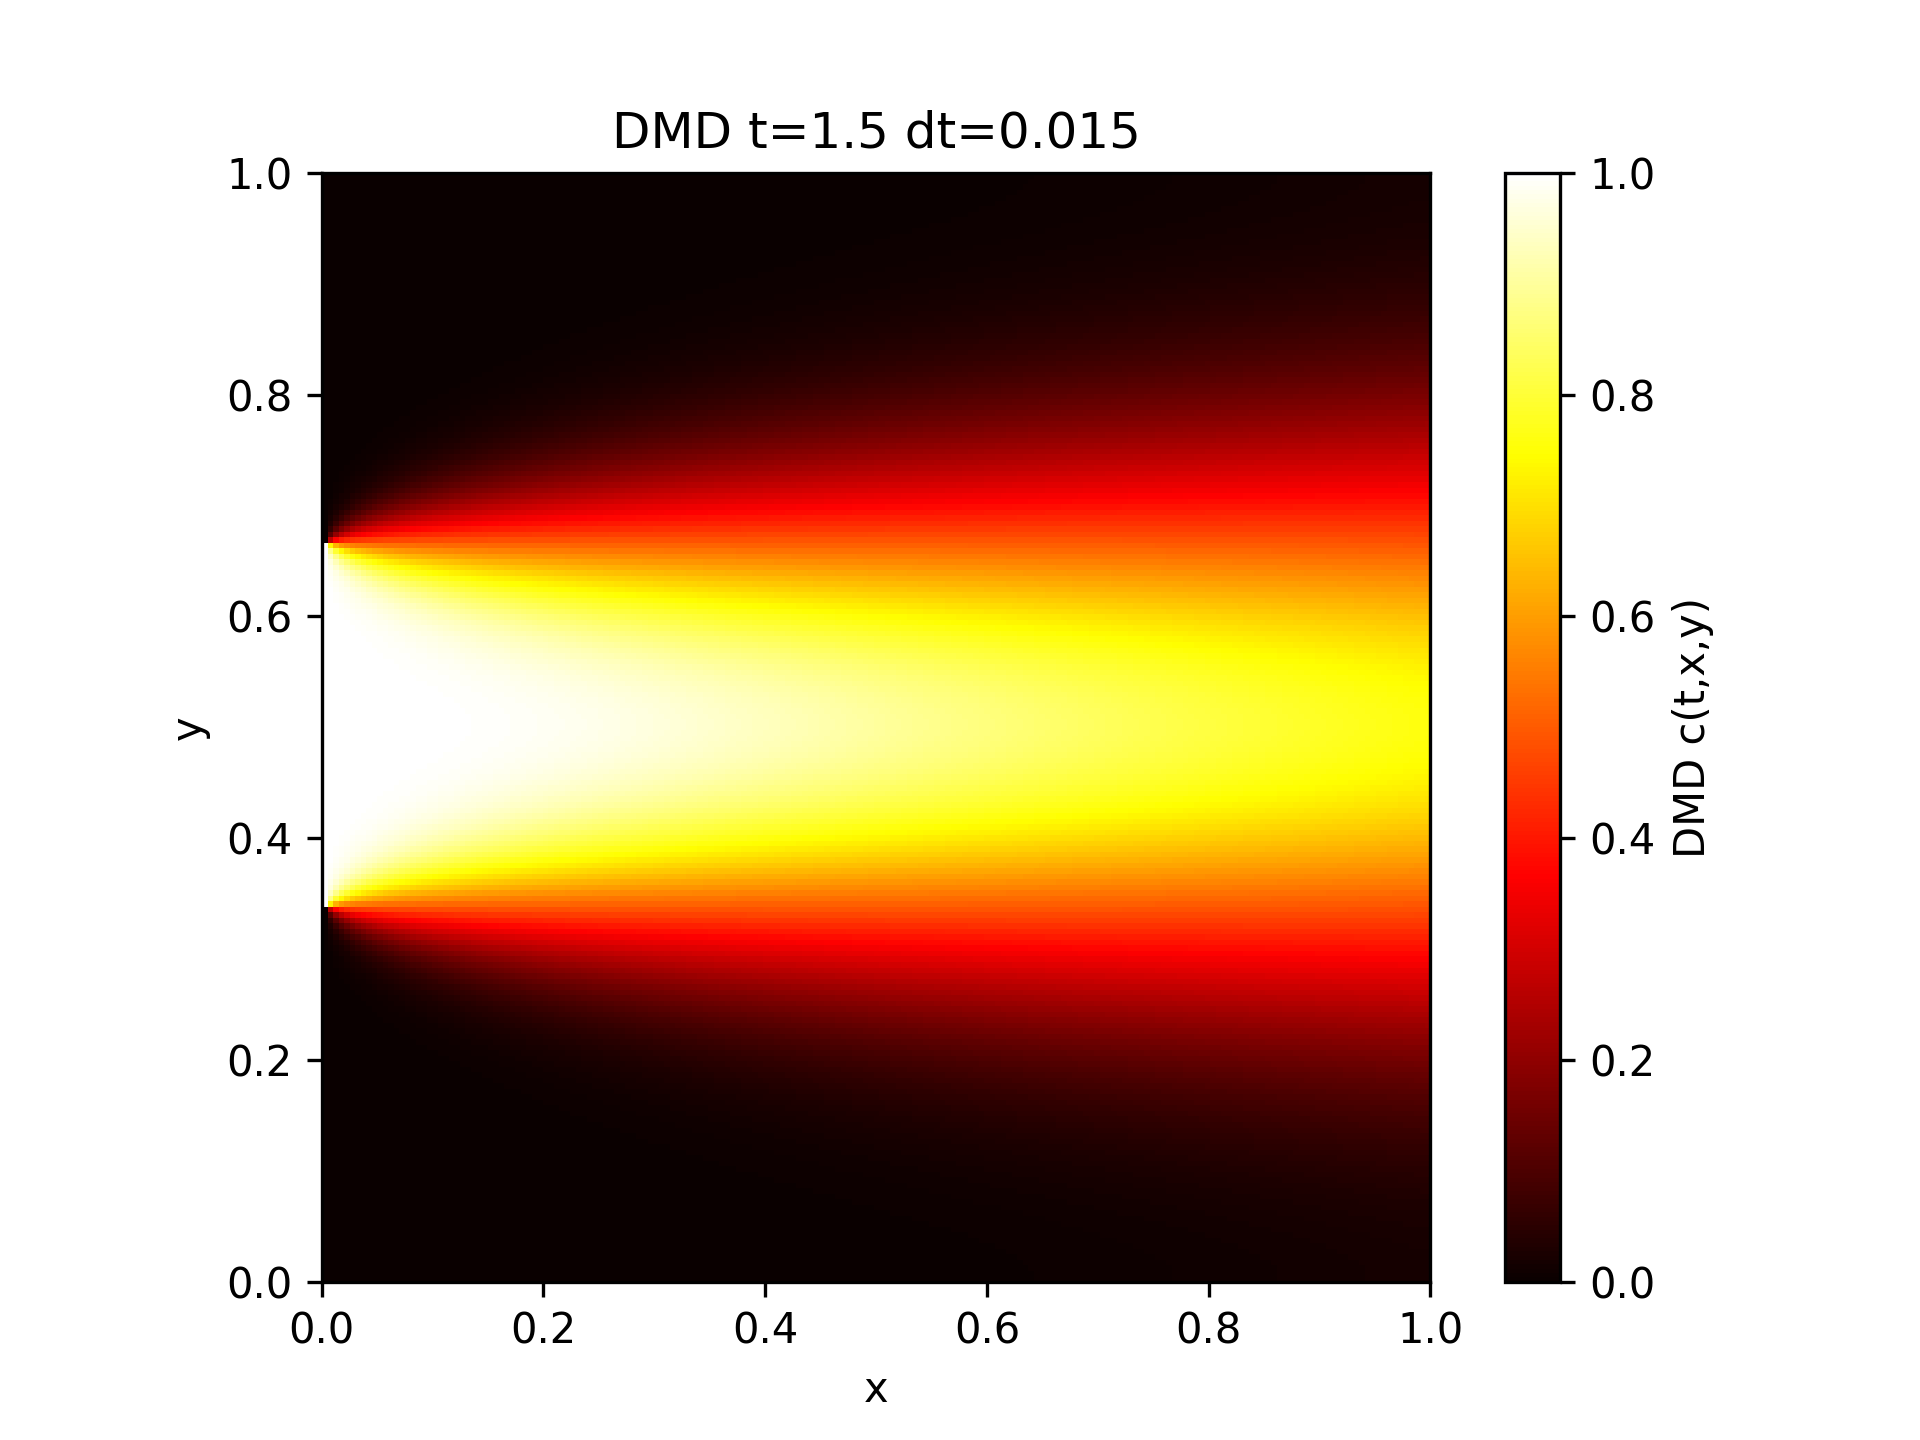
\includegraphics[width=\textwidth]{DMD t=1.5 dt=0.015.png}
        \caption{DMD t=1.5 dt=0.015}
        \label{DMD t=1.5 dt=0.015}
    \end{subfigure}
    \caption{results of DMD dt = 0.015}
    \label{results of DMD dt = 0.015}
\end{figure}
\end{document}